\documentclass[twoside, 12pt]{article}

\usepackage[sc]{mathpazo} % Use the Palatino font
\usepackage[T1]{fontenc} % Use 8-bit encoding that has 256 glyphs
\linespread{1.5} % Line spacing - Palatino needs more space between lines

%\usepackage[twoside,width=16cm,height=24cm,left=3cm]{geometry}
\usepackage[margin=2cm]{geometry} % Document margins
\usepackage{multicol} % Used for the two-column layout of the document
\usepackage[hang, small,labelfont=bf,up,textfont=it,up]{caption} % Custom captions under/above floats in tables or figures
\usepackage{booktabs} % Horizontal rules in tables
\usepackage{float} % Required for tables and figures in the multi-column environment - they need to be placed in specific locations with the [H] (e.g. \begin{table}[H])
\usepackage{hyperref} % For hyperlinks in the PDF

%----------- Agregados para el caso de ustedes -------------------------------
\usepackage[spanish]{babel}% idioma castellano
\usepackage[utf8]{inputenc}% esto es para poder poner los tildes directamente. Puede que cambie de versión a versión de sistema operativos (más información en http://www.aq.upm.es/Departamentos/Fisica/agmartin/webpublico/latex/FAQ-CervanTeX/FAQ-CervanTeX-6.html )
\usepackage{graphicx} % para insertar figuras
\usepackage{subfigure} % para insertar figuras dentro de figuras
\usepackage{times} % plataforma
\usepackage{amsmath} % --para ecuaciones y algunos símbolos
\usepackage{wrapfig,lipsum}
\usepackage{listings}
\usepackage{color}
\usepackage{braket}
\usepackage{amsthm}
\usepackage{cancel}

\definecolor{dkgreen}{rgb}{0,0.6,0}
\definecolor{gray}{rgb}{0.5,0.5,0.5}
\definecolor{mauve}{rgb}{0.58,0,0.82}

\lstset{frame=tb,
	language=C++,
	aboveskip=3mm,
	belowskip=3mm,
	showstringspaces=false,
	columns=flexible,
	basicstyle={\small\ttfamily},
	numbers=none,
	numberstyle=\tiny\color{gray},
	keywordstyle=\color{blue},
	commentstyle=\color{dkgreen},
	stringstyle=\color{mauve},
	breaklines=true,
	breakatwhitespace=true,
	tabsize=3
}
% ---------------------- -----------------------------------------------------

\usepackage{lettrine} % The lettrine is the first enlarged letter at the beginning of the text
\usepackage{paralist} % Used for the compactitem environment which makes bullet points with less space between them
\usepackage[T1]{fontenc}					%para poder usar tildes sin problemas

\usepackage{mathrsfs}
% Abreviaturas
%\newcommand\RR{\mathbb{R}}

\newtheorem{theorem}{Theorem}
\providecommand{\dpart}[2]{\frac{\partial#1}{\partial#2}}
\providecommand{\poisson}[2]{\left\{#1; #2 \right\}_{Poisson}}

\graphicspath{{Imagenes/}}

\begin{document}

\section{Introducción}
 \subsection{Gas de Fermi}{\label{sec:intro_fermi_gas}}

En los sistemas cuánticos, la indistingubilidad de las particulas juega un rol esencial.
Esta indistingubilidad obliga a todos los autoestados $\ket{\psi}$ del sistema a ser autoestados del operador permutación de 2 partículas $\hat{P}$, cuyos únicos autovalores son $\pm 1$.
De esta manera, se asegura la invarianza de los observables ante $\hat{P}$
\[\bra{\psi'}\hat{A}\ket{\psi'} = \bra{\psi}\hat{P}^\dagger\hat{A}\hat{P}\ket{\psi} = (\bra{\psi}\pm)\hat{A}(\pm\ket{\psi}) = \bra{\psi}\hat{A}\ket{\psi}\]

Los fermiones son aquellas particulas cuyas funciones de onda tienen autovalor negativo ante cualquier permutación de 2 partículas ($\hat{A}\ket{\psi} = -\ket{\psi}$) y se dice que son antisimétricas.
De esta propiedad surge el principio de exclusión de Pauli, que prohibe la ocupación de un mismo estado por más de una partícula. 
De otra forma, sería imposible lograr que la función de onda sea antisimétrica, dado que si tuviesemos dos partículas $i$ y $j$ en el mismo estado, la permutación $\hat{P}_{ij}$ mantendría
$\ket{\psi}$ invariante en lugar de cambiar su signo.

En general, los fermiones poseen spin semi-entero $s=l+1/2$, razón por la que los nucleones (protones y neutrones) y los electrones son fermiones. 
La exclusión de Pauli tiene efectos importantes en la termodinámica de fermiones a bajas temperaturas.
El sistema de fermiones no interactuantes es el más simple, cuya estadística es bien conocida, siendo su función de partición gran canónica y ocupación media
\begin{equation}
 \frac{PV}{k_BT} \equiv \log Z = \sum_\varepsilon \log(1+ze^{-\beta\varepsilon})
\end{equation}
\begin{equation}
 N = \sum_\varepsilon \langle n_\varepsilon\rangle = \sum_\varepsilon \frac{1}{z^{-1}e^{\beta\varepsilon}+1}
\end{equation}
con $z=e^{\beta\mu}$ la fugacidad, $\beta=1/k_BT$ y $\mu$ el potencial químico del sistema. 
Los niveles de energía de una partícula $\varepsilon=p^2/2m$ están discretizados y dependen del volumen $V$, con $\Delta\varepsilon\sim V^{-1/3}$.

En el límite termodinámico ($V\to\infty$), la diferencia entre energías $\Delta\varepsilon\to 0$ y podemos transformar la sumatoria en una integral en el espacio de fases.
Realizando las integrales triviales, resulta
\begin{equation}
 \frac{PV}{k_BT} \equiv \log Z = \frac{4\pi V}{h^3} \int_0^\infty \log(1+ze^{-\beta p^2/2m})p^2dp = \frac{gV}{\lambda^3}f_{5/2}(z)
\end{equation}
\begin{equation}{\label{eq:N_cont}}
 N = \frac{4\pi V}{h^3} \int_0^\infty \frac{1}{z^{-1}e^{\beta p^2/2m}+1} p^2dp = \frac{gV}{\lambda^3}f_{3/2}(z)
\end{equation}
donde $g$ es un factor de degeneración asociado a grados de libertad internos (spin, por ejemplo) y  $\lambda$ es la longitud de onda térmica
\[ \lambda = \sqrt{ \frac{2\pi\hbar^2}{mk_BT} } \]
y las $f_\nu(z)$ son las funciones de Fermi-Dirac definidas según
\[ f_\nu(z) = \frac{1}{\Gamma(\nu)}\int_0^\infty \frac{x^{\nu-1}}{z^{-1}e^x+1} = \sum_{l=1}^\infty (-1)^{l+1}\frac{z^l}{l^\nu}\]

Para un sistema NVT, debemos obtener la fugacidad $z$ invirtiendo \eqref{eq:N_cont}, lo que introduce el problema de computar las funciones de Fermi-Dirac $f_\nu(z)$.
Al ser series alternadas, la convergencia de las sumas parciales es muy lenta y debemos recurrir a otros métodos, que detallamos en el Apéndice \textbf{APENDICE DIRAC}.
Independientemente de esto, puede verse que obtendremos un $\mu(N/V,T) = \mu(\rho, T)$, razonable dado que es una magnitud intensiva del sistema.

El integrando de \eqref{eq:N_cont} puede considerarse como la densidad de partículas $f(p)$ con impulso de módulo $p$.
Esta distribución de impulsos es característica de un gas de fermiones isótropo y homogéneo.
Equivalentemente, podriamos analizar la distrubición de energías cinéticas $\varepsilon=p^2/2m$ mediante un cambio de variables sobre la integral de \eqref{eq:N_cont} 
($d\varepsilon = pdp/m = \sqrt{2m\varepsilon}dp/m$)

\[ N = \frac{4\pi V}{h^3} \int_0^\infty \frac{1}{e^{\beta(\varepsilon-\mu)}+1} 2m\varepsilon\frac{m}{\sqrt{2m\varepsilon}}d\varepsilon = 
\int_0^\infty \frac{4\pi V\sqrt{2m^3\varepsilon}}{h^3}\frac{1}{e^{\beta(\varepsilon-\mu)}+1} d\varepsilon\]

Por lo tanto, la distribución de impulsos toma la forma 
\begin{equation}{\label{eq:dist_FD}}
 f_{FD}(\varepsilon) = \frac{4\pi V \sqrt{2m^3\varepsilon}}{h^3}\frac{1}{e^{\beta(\varepsilon-\mu)}+1} = \frac{G(\varepsilon)}{e^{\beta(\varepsilon-\mu)}+1} 
 %= N\frac{V}{\lambda^3}\sqrt{\frac{4\beta^3\varepsilon}{\pi}}\frac{1}{e^{\beta(\varepsilon-\mu)}+1} 
\end{equation}
donde $G(\varepsilon)$ es la degeneración de estados con energía $\varepsilon$ y asumimos $\mu=\mu(N,V,T)$.

En el límite de altas temperaturas (o baja densidad), esperamos que el sistema pierda sus propiedades cuánticas y recuperemos el gas clásico, donde las partículas
se vuelven distinguibles nuevamente. 
La noción de alta temperatura (o baja densidad) viene dada por el valor del producto $\lambda^3\rho \sim T^{-3/2}\rho$, donde vemos que $T\to\infty$ resulta equivalente a $\rho\to0$ 
y viceversa para baja temperatura (o alta densidad), donde las propiedades cuánticas son más apreciables.

Para un sistema de partículas clásico interactuando con potenciales dependientes de la posición $U(\mathbf{q}_1,..,\mathbf{q}_N)$, la distribución de impulsos 
corresponde a la de Boltzmann (ver \textbf{Apéndice \ref{ap:boltzmann}}).
\begin{equation}{\label{eq:dist_MB}}
 f_{MB}(\varepsilon) = N\sqrt{\frac{4\beta^3\varepsilon}{\pi}}e^{-\beta\varepsilon}
\end{equation}


\subsection{Potencial de Pauli}

Dado que la distribución \eqref{eq:dist_MB} es común a todo sistema de partículas distinguibles (o clásicas) cuyos Hamiltonianos cuya dependencia con el momento 
sea a través de la energía cinética (ver  \textbf{Apéndice \ref{ap:boltzmann}})
\[ H(\mathbf{q}_1,..,\mathbf{q}_N,\mathbf{p}_1,..,\mathbf{p}_N) = \sum_i \frac{p_i^2}{2m} + U(\mathbf{q}_1,..,\mathbf{q}_N)\]
la única forma de obtener una distribución de energías distinta con partículas distinguibles es introduciendo potenciales dependientes de momentos al Hamiltoniano. 

Esto puede hacerse de infinitas maneras, pero en particular buscamos una cuya distribución resulte similar a \eqref{eq:dist_FD}.
Para esto, necesitamos poder expresar la noción de Exclusión de Pauli con un potencial de interacción de dos partículas $V(\mathbf{q}_1,..,\mathbf{q}_N;\mathbf{p}_1,..,\mathbf{p}_N)$.
Esto lo haremos imponiendo un ``costo energético'' cada vez que 2 partículas tengan un $\mathbf{q}, \mathbf{p}$ similar. 
Buscamos lograr esto agregando al Hamiltoneano un potencial de interacción de 2 partículas que llamaremos \textit{potencial de Pauli} definido según

\begin{equation}{\label{eq:def_int_pauli}}
 V_P(\mathbf{q}_1,\mathbf{q}_2;\mathbf{p}_1,\mathbf{p}_2) = De^{-\frac{1}{2}\left( \frac{|\mathbf{q}_1-\mathbf{q}_2|^2}{q_o^2} +\frac{|\mathbf{p}_1-\mathbf{p}_2|^2}{p_o^2} \right)}
\end{equation}
donde surge la noción de distancia en el espacio de fases $s^2 = \frac{|\mathbf{q}_1-\mathbf{q}_2|^2}{q_o^2} +\frac{|\mathbf{p}_1-\mathbf{p}_2|^2}{p_o^2}$. 

Podemos visualizar los parámetros $q_o$ y $p_o$ como los ejes de un elipsoide en $\mathbb{R}^6$ (el espacio de fases) donde $s^2 \leq 1$ y el costo energético de cualquier partícula 
que ingrese es $\approx D$.
A energías (o temperaturas) bajas, este costo energético puede ser suficientemente alto como para evitar la superposición de estos elipsoides en el espacio de fases, generando efectivamente
la noción de exclusión de Pauli: dos partículas no pueden estar en el mismo estado $(\mathbf{q}, \mathbf{p})$.
Es importante notar que este potencial no es de núcleo duro y, por lo tanto, es posible que dos partículas se superpongan para energías suficientemente altas donde $D$ sea despreciable.
Esto es deseable dado que para energías (o temperaturas) altas esperamos recuperar el gas clásico de Maxwell-Boltzmann al desaparecer $V_P$.

Este potencial fue inicialmente propuesto por 

\subsection{Integración simpléctica de sistemas hamiltonianos}

La evolución de las $d$ coordenadas generalizadas $q \equiv (q_1,..,q_d)\in\mathbb{R}^{d}$ y $p \equiv (p_1,..,p_d)\in\mathbb{R}^{d}$ está definida por el Hamiltoneano
$H(q_1,..,q_d,p_1,..,p_d) \equiv H(q,p)$  a través de las ecuaciones de Hamilton
\begin{align*}
 \dot{q} &= \dpart{H}{p}(q,p) \\
 \dot{p} &= -\dpart{H}{q}(q,p)
\end{align*}
que podemos compactar definiendo $y=(p,q)\in\mathbb{R}^{2d}$ y la matriz $J = \begin{pmatrix}0 & \mathbb{I} \\-\mathbb{I} & 0\end{pmatrix}$ (con la propiedad $J^{-1} = J^T = -J$)
\begin{equation}{\label{eq:ec_hamilton}}
 \dot{y} = J^{-1}\nabla H(y)
\end{equation}

Para un Hamiltoneano que no depende explícitamente del tiempo, la ecuación de evolución \ref{eq:ec_hamilton} asegura la conservación de $H(q,p)$ en el tiempo 
\[ \frac{dH}{dt}(y) = \nabla H(y)\cdot \dot{y} = \nabla H(y)^T J^{-1}\nabla H(y) = 0\]
donde usamos que $(a,b)J^{-1}\begin{pmatrix}a\\b\end{pmatrix} = (b, -a)\begin{pmatrix}a\\b\end{pmatrix} = 0$ $\forall a,b$.
Esto no es más que la conocida conservación de la energía.

\subsubsection{Transformaciones simplécticas}{\label{sec:trans_simp}}

Sin embargo, los sistemas hamiltoneanos tienen propiedades adicionales asociadas a la conservación del área en el espacio de fases de $y$. 
Supongamos dos vectores 
\[ \mu = \begin{pmatrix} \mu^p\\ \mu^q \end{pmatrix} \qquad \eta = \begin{pmatrix} \eta^p\\ \eta^q \end{pmatrix}  \]
con $\mu^p, \mu^q, \eta^p, \eta^q\in\mathbf{R}^{d}$ las ``componentes $p$ y $q$'' de estos vectores.
Definimos el mapeo bilinear $\omega(\mu,\eta)$ como la suma de las areas orientadas de cada par de componentes $p_i,q_i$ 
\begin{equation}
 \omega(\mu, \eta) = \sum_{i=1}^{3N} \det \begin{pmatrix} \mu^p_i & \eta^p_i \\ \mu^q_i & \eta^q_i \end{pmatrix} = \sum_{i=1}^{3N} \mu^p_i\eta^q_i - \mu^q_i\eta^p_i = \mu^T J \eta
\end{equation}

Con esta noción de área, decimos que un mapeo diferenciable $g:U\subseteq\mathbb{R}^{2d}\to\mathbb{R}^{2d}$ es \textit{simpléctico} si su matriz jacobiana $g'(p,q)$ cumple alguna de las condiciones
equivalentes \[ g'(p,q)^T J g'(p,q) = J \qquad \text{ o } \qquad \omega(g'(p,q)\mu, g'(p,q)\eta) = \omega(\mu, \eta) \]

Para visualizar esto, supongamos $M$ una subvariedad de dimensión 2 de $U$ parametrizada por alguna función suave $\psi(s,t)$ tal que $M=\psi(K)$ para $K\subseteq\mathbb{R}^2$.
Podemos considerar a $M$ como la unión de infinitos paralelogramos infinitesimales definidos por los vectores
\[ \dpart{\psi}{s}(s,t)ds \quad \text{ y } \quad \dpart{\psi}{t}(s,t)dt \]

Sumando sobre todos estos paralogramos, obtenemos el área de $M$ como
\begin{equation}{\label{eq:area_orien_simp}}
 \Omega(M) = \iint_K \omega\left(\dpart{\psi}{t}(s,t), \dpart{\psi}{s}(s,t)\right) ds dt
\end{equation}
y resulta inmediato ver que este volumen es invariante ante una transformación simpléctica $g$.

\begin{theorem}{\label{teo:preservacion_vol}}
 Sea un mapeo diferenciable $g:U\subseteq\mathbb{R}^{2d}\to\mathbb{R}^{2d}$ simpléctico. Luego, preserva $\Omega(M)$ 
 \[ \Omega(g(M)) = \Omega(M) \]
 para toda variedad $M\subseteq\mathbb{R}^2$ que pueda representarse como la imagen de una función diferenciable $\psi$.
\end{theorem}
\begin{proof}
\begin{align*}
 \Omega(g(M)) &=  \iint_K \omega\left(\dpart{(g\circ\psi)}{t}(s,t), \dpart{(g\circ\psi)}{s}(s,t)\right) ds dt \\
&= \iint_K \omega\left(g'(\psi(s,t))\dpart{\psi}{t}(s,t), g'(\psi(s,t))\dpart{\psi}{s}(s,t)\right) ds dt = \iint_K \omega\left(\dpart{\psi}{t}(s,t), \dpart{\psi}{s}(s,t)\right) ds dt = \Omega(M) 
\end{align*}
donde utilizamos la propiedad de $g$ simpléctica. 
\end{proof}

Finalmente, nos basta ver que el mapeo de evolución temporal $\varphi_t(p_o,q_o) = (p(t;p_o,q_o), q(t;p_o,q_o))$ donde $p(t;p_o,q_o), q(t;p_o,q_o)$ son las soluciones de \eqref{eq:ec_hamilton}
con condiciones iniciales $p(0)=p_o$ y $q(0)=q_o$. 
Reemplazando $y$ por $\varphi_t(p_o,q_o)$ en \eqref{eq:ec_hamilton} y derivando respecto de $y_o=(p_o,q_o)$ tenemos
\begin{align*}
 \dpart{\dot{\varphi_t}}{y_o} &= J^{-1}\dpart{}{y_o} \nabla H(\varphi_t) \\
 \frac{d}{dt}\left(\dpart{\varphi_t}{y_o}\right) &= J^{-1} \nabla^2 H(\varphi_t)\dpart{\varphi_t}{y_o}
\end{align*}

donde $\nabla^2 H$ es la matriz hessiana de $H$ y, cabe destacar, es simétrica. Esta propiedad es esencial, pues de ella se deriva el siguiente teorema
 
\begin{theorem}{\label{teo:preservacion_evol}}
  Sea $H(p,q)$ una función doblemente diferenciable en $U\subseteq\mathbb{R}^{2d}$. Luego, para cada $t$ fijo, el mapeo $\varphi_t$ es una transformación simpléctica
  para cualquier condición inicial $y_o$.
\end{theorem}
\begin{proof}
 Para este caso, tenemos $g'(p,q) = \dpart{\varphi_t}{y_o}(y_o)$ y, por lo tanto,
 \begin{align*}
  \frac{d}{dt}\left[ \left(\dpart{\varphi_t}{y_o}\right)^T J \left(\dpart{\varphi_t}{y_o}\right) \right] 
  &= \left[\frac{d}{dt}\left(\dpart{\varphi_t}{y_o}\right)^T\right] J \left(\dpart{\varphi_t}{y_o}\right) + \left(\dpart{\varphi_t}{y_o}\right)^T J \left[\frac{d}{dt}\left(\dpart{\varphi_t}{y_o}\right)\right] \\
  &= \left[J^{-1} \nabla^2 H(\varphi_t)\dpart{\varphi_t}{y_o}\right]^T J \left(\dpart{\varphi_t}{y_o}\right) + \left(\dpart{\varphi_t}{y_o}\right)^T J \left[J^{-1} \nabla^2 H(\varphi_t)\dpart{\varphi_t}{y_o}\right] \\  
  &= \left(\dpart{\varphi_t}{y_o}\right)\nabla^2 H(\varphi_t)\left(J^{-1} \right)^T J \left(\dpart{\varphi_t}{y_o}\right) + \left(\dpart{\varphi_t}{y_o}\right)^T \nabla^2 H(\varphi_t)\dpart{\varphi_t}{y_o} = 0 
 \end{align*}
 donde usamos que $J^{-1} = J^T$ y $J^2 = -\mathbb{I}$.
 
 Por lo tanto, $\left(\dpart{\varphi_t}{y_o}\right)^T J \left(\dpart{\varphi_t}{y_o}\right)$ es constante $\forall t$ y para $t=0$ tenemos $\varphi_0(y_o) = y_o$ por lo que $\dpart{\varphi_0}{y_o}=\mathbb{I}$
 \[ \left(\dpart{\varphi_t}{y_o}\right)^T J \left(\dpart{\varphi_t}{y_o}\right) = \left(\dpart{\varphi_o}{y_o}\right)^T J \left(\dpart{\varphi_o}{y_o}\right) = \mathbb{I}^T J \mathbb{I} = J\]
\end{proof}


\subsubsection{Integradores simplécticos}{\label{sec:int_simpl}}

Dado que la simplecticidad es una propiedad fundamental de todo sistema hamiltoneano, resulta razonable plantear que el integrador que utilicemos para evolucionar temporalmente 
el sistema también lo sea. 
Consideramos un integrador de un paso es simpléctico si el mapeo asociado $y_1=\Phi_h(y_o)$ es simpléctico. 

El primer integrador simpléctico de interés es \textit{MidPoint Rule} (MPR), cuyo esquema es 
\begin{equation}{\label{eq:MPR}}
 y_{n+1} = y_n + hJ^{-1}\nabla H\left(\frac{y_{n+1}+y_n}{2}\right)
\end{equation}
 
Veamos que es de orden 2 tomando $y(t_o+h)$ como la solución exacta a \eqref{eq:ec_hamilton} con $y(t_o)=y_o$
\[ y(t_o+h) = y_o + hJ^{-1}\nabla H(y_o) + O(h^2) \]
\[ y_1 = y_o + hJ^{-1}\nabla H\left(\frac{y_1+y_o}{2}\right) =  y_o + hJ^{-1}\nabla H\left(y_o + \frac{h}{2}J^{-1}\nabla H\left(\frac{y_1+y_o}{2}\right)\right) = y_o + hJ^{-1}\nabla H(y_o) + O(h^2) \]
\[ y(t_o+h) - y_1 = O(h^2) \]
por lo que resulta de orden mayor a 1. 
Sin embargo, el esquema de MPR es \textit{simétrico} dado que se mantiene al hacer el cambio $y_{n+1}\to y_n$, $y_n\to y_{n+1}$ y $h\to -h$.
Como todo integrador simétrico debe tener orden par, entonces MPR resulta de orden 2 (o superior).

Además, podemos probar que este esquema es simpléctico
\[ \dpart{y_{n+1}}{y_n} = 1 + hJ^{-1}\dpart{}{y_n} \nabla H\left(\frac{y_{n+1}+y_n}{2}\right) = 1 + hJ^{-1} \nabla^2H\left(\frac{y_{n+1}+y_n}{2}\right)\frac{1}{2}\left[ 1+\dpart{y_{n+1}}{y_n} \right]\]
\[ \left[ 1 - \frac{h}{2}J^{-1} \nabla^2H\left(\frac{y_{n+1}+y_n}{2}\right) \right]\dpart{y_{n+1}}{y_n} =  1 + \frac{h}{2}J^{-1} \nabla^2H\left(\frac{y_{n+1}+y_n}{2}\right)\]
donde representamos la identidad de $\mathbb{R}^{2d}$ $\mathbb{I}=1$. 
Definiendo $E\equiv\frac{h}{2}J^{-1} \nabla^2H\left(\frac{y_{n+1}+y_n}{2}\right)$ podemos despejar $\dpart{y_{n+1}}{y_n}$ 
\[ \dpart{y_{n+1}}{y_n} = (1-E)^{-1}(1+E) \]

Buscamos ver que $\left(\dpart{y_{n+1}}{y_n}\right)^TJ\left(\dpart{y_{n+1}}{y_n}\right)= J$, pero antes mostraremos una propiedad útil de $J$ y $E$
\[ E^T J = \frac{h}{2}\left( J^{-1} \nabla^2H \right)^T J = \frac{h}{2} \nabla^2H(J^{-1})^T  J = -\frac{h}{2} \nabla^2H = -JE\]
\[ (1 + E^T)^{-1}J = \sum_{n\geq0} \left(E^T\right)^n J = J\sum_{n\geq0} (-1)^nE^n = J(1 - E)^{-1}  \]

Ahora si podemos probar la simplecticidad de MPR
\[ \left(\dpart{y_{n+1}}{y_n}\right)^TJ\left(\dpart{y_{n+1}}{y_n}\right) = (1+E^T)(1-E^T)^{-1}J(1-E)^{-1}(1+E) = J(1-E)(1+E)^{-1}(1-E)^{-1}(1+E) = J\]

Sin embargo, es inmediato notar que el esquema de MPR no es explícito; no es posible obtener $y_{n+1}$ como una combinación de funciones conocidas aplicadas a $y_n$.
Otro método simpléctico ampliamente utilizado es \textit{Velocity-Verlet} que,a demás de tener el mismo orden resulta explícito para hamiltoneanos separables
\[ H(\mathbf{q}_1,..,\mathbf{q}_N,\mathbf{p}_1,..,\mathbf{p}_N) = \sum_i \frac{p_i^2}{2m} + U(\mathbf{q}_1,..,\mathbf{q}_N)\]

El esquema tiene dos versiones, pero la más utilizada (y que resulta explícita) es
\begin{align*}
 p_{n+1/2} &= p_n - \frac{h}{2}\dpart{H}{q}(p_{n+1/2}, q_n) \\
 q_{n+1} &= q_n + \frac{h}{2}\left( \dpart{H}{p}(p_{n+1/2}, q_n) + \dpart{H}{p}(p_{n+1/2}, q_{n+1}) \right) \\
 p_{n+1} &= p_{n+1/2} - \frac{h}{2}\dpart{H}{q}(p_{n+1/2}, q_{n+1})
\end{align*}
que para estos hamiltoneanos resulta explicitamente
\begin{align*}
 p_{n+1/2} &= p_n - \frac{h}{2}\dpart{U}{q}(q_n) \\
 q_{n+1} &= q_n + \frac{h}{m}p_{n+1/2} \\
 p_{n+1} &= p_{n+1/2} - \frac{h}{2}\dpart{U}{q}(q_{n+1}) = p_n - \frac{h}{2} \left( \dpart{U}{q}(q_n) + \dpart{U}{q}(q_{n+1}) \right)
\end{align*}

Sin embargo, para hamiltoneanos de la forma
\[ H(\mathbf{q}_1,..,\mathbf{q}_N,\mathbf{p}_1,..,\mathbf{p}_N) = \sum_i \frac{p_i^2}{2m} + U(\mathbf{q}_1,..,\mathbf{q}_N;\mathbf{p}_1,..,\mathbf{p}_N)\]
se vuelve nuevamente implícito. 
Esta es una característica común a todos los integradores simplécticos: solo resultan explícitos para hamiltoneanos separables.

Esto resulta muy relevante, dado que implica que el uso de Dinámica Molecular para sistemas interactuantes mediante potencial de Pauli requerirá además la implementación
de algún método para resolver ecuaciones implícitas como \eqref{eq:MPR}.
El costo computacional de estas implementaciones resulta prohibitivo para sistemas de muchas partículas, como mostraremos más adelante. 



\subsection{Método de Metropolis-Montecarlo}

En principio, conocer la función de partición $Z$ otorga acceso a todas las magnitudes termodinámicas de interés.
Para un sistema de $N$ partículas no interactuantes, el hamiltoniano total del sistema puede escribirse como la suma de hamiltonianos de una partícula
\[H(\mathbf{q}_1,..,\mathbf{q}_N;\mathbf{p}_1,..,\mathbf{p}_N) = H_1(\mathbf{q}_1, \mathbf{p}_1) + ... +H_N(\mathbf{q}_N, \mathbf{p}_N)\] 
lo cual permite inmediatamente factorizar la función de partición canónica
\[ Z = \int e^{-\beta H(\mathbf{q}_1,..,\mathbf{q}_N;\mathbf{p}_1,..,\mathbf{p}_N)} d^{3N}qd^{3N}p = \prod_{i=1}^N \int e^{-\beta H_i(\mathbf{q};\mathbf{p})} d^{3}qd^{3}p = \prod_{i=1}^N Z_i \]

En general, habrá $n\ll N$ funciones de partición distintas, donde $n$ es la cantidad de tipos de partículas (equivalentemente, la cantidad de hamiltonianos diferentes) y el computo de $Z$ resulta simple.

Para sistemas interactuantes, este método no es aplicable al no ser el hamiltoniano separable; excepto en casos particulares, el cálculo de $Z$ para sistemas interactuantes resulta analíticamente imposible. 
Aunque calcular los pesos $e^{-\beta H(\mathbf{q}_1,..,\mathbf{q}_N;\mathbf{p}_1,..,\mathbf{p}_N)}$ para una dada configuración es posible, el cómputo de $Z$ exige barrer el espacio de fases $6N$-dimensional, 
cuyo volumen crece exponencialmente con $N$.

Para temperaturas finitas, sin embargo, gran parte de este volumen generará un aporte ínfimo a la función de partición $Z$, al ser estados cuyo peso relativo es bajo. 
Por esto mismo, tendrán un aporte ínfimo en los valores medios de las magnitudes termodinámicas de interés. 
Por lo tanto, buscamos un método que nos permita evitar por completo el cómputo de $Z$ y tome en cuenta solo las configuraciones relevantes para el sistema a una dada temperatura $T$.
El método de Metropolis-Montecarlo (también conocido como Metropolis-Hastings) nos permite lograr esto mediante el uso de cadenas de Markov.

\subsubsection{Cadenas de Markov}

Las cadenas de Markov son ampliamente utilizadas para modelar múltiples fenómenos (biologicos, economicos, sociales) por su simplicidad y teoría bien desarrollada.
El objetivo de las cadenas de Markov es introducir la memoria en una sucesión de variables aleatorias $(X_n)_{n\in \mathbb{N}}$ de la forma más simple posible.
Esto es, la evolución $X_n \to X_{n+1}$ no depende de los $n-1$ estados previos ni del 'tiempo' $n$, sino únicamente del estado actual $X_n$.

Con esto en mente, una sucesión de variables aleatorias $(X_n)_{n\in \mathbb{N}}$ es una cadena de Markov a tiempo discreto si
\[ P(X_{n+1}=j | X_n = i, X_{n-1} = i_{n-1}, ..., X_o = i_0) = P(X_{n+1}=j | X_n = i)  \]
donde $j, i, i_{n-1}, ..., i_0$ son estados posibles de la cadena. 

Se define la matriz de transición $p(i,j)$ de la cadena de Markov como la probabilidad de alcanzar el estado $j$ partiendo del estado $i$, aprovechando la independencia del tiempo $n$
\[ p(i,j) = P(X_{n+1} = j | X_n = i) \]

En particular, si nos interesa ver las probabilidades de transición múltiples pasos adelante (a $n$ pasos)
\begin{align*}
 p_n(i,j) = P(X_n = j | X_0 = i) &= \frac{P(X_n = j, X_0 = i)}{P(X_0 = i)} \\
 &= \sum_k \frac{P(X_n = j, X_{n-1}=k, X_0 = i)}{P(X_0 = i)} \\
 &= \sum_k P(X_n = j| X_{n-1}=k, X_0 = i)\frac{P(X_{n-1}=k, X_0 = i)}{P(X_0 = i)} \\
 &= \sum_k P(X_n = j| X_{n-1}=k)P(X_{n-1}=k| X_0 = i) = \sum_k p(k,j)p_{n-1}(i,k)
\end{align*}

Identificando la suma anterior como el producto de matrices $(p_{n-1} \cdot p)(i,j)$ y usando que $p_1(i,j)=p(i,j)$, resulta inmediato que $p_n(i,j) = p^n(i,j)$. 
En esta propiedad reside la simplicidad de las cadenas de Markov.

En particular, nos interesan las cadenas de Markov irreducibles; aquellas en las que todo estado $i$ puede alcanzar el estado $j$ en una cantidad finita de pasos.
Matemáticamente, decimos que una cadena de Markov es irreducible si
\[ \forall i,j \quad \exists n\in \mathbb{N} \text{ tal que } p^n(i,j) \neq 0 \]

El caso más simple de una cadena no irreducible es una con dos conjuntos de estados $A$ y $B$ desconectados entre si.
\[ p = 
\begin{pmatrix}
 p_A & 0\\ 
 0 & p_B
\end{pmatrix} \]
En estos casos, resultaría mucho más sensato tratarla como dos cadenas de Markov de estados $A$ y $B$ con sus respectivas matrices $p_A$ y $p_B$.

El otro caso de cadena no irreducible es aquella con estados absorventes; aquellos que no pueden transicionar a otros estados.
Decimos que un estado $i$ es absorvente si $p(i,j)=\delta_{ij} \text{ } \forall j$.
Estas cadenas, en principio, pueden utilizarse para modelar ciertos problemas como la 'Ruina del jugador'. (¿NOTA AL PIE?)

En el método de Montecarlo, las cadenas de Markov utilizadas son irreducibles dado que tienen lo que se conoce como una \textit{distribución estacionaria}, que describimos a continuación.

\subsubsection{Distribución estacionaria}

Cuando el estado inicial de una cadena de Markov tiene una distribución $q(i)$, podemos usar el resultado anterior para calcular la distribución $n$ pasos después
\[ P(X_n=j) = \sum_i P(X_n=j,X_0=i) =  \sum_i P(X_n=j|X_0=i)P(X_0=i) = \sum_i p^n(i,j)q(i) = (q\cdot p^n)(j)\]
usando el producto habitual de matrices y tomando el vector fila de probabilidades $q$.
Por lo tanto, la distribución de probabilidad a tiempo $n$ se relaciona con la inicial segun $q_n = q_0\cdot p^n$ o, recursivamente, $q_{n+1} = q_n\cdot p$.

Resulta natural entonces preguntarse si existirá alguna forma de mantener la distribución constante $q_{n+1} = q_n$.
Esto es equivalente a pedir que $q_n$ sea un autovector de $p$ con autovalor 1. 
Para diferenciar, llamaremos $\pi(x)$ a esta distribución estacionaria que cumple $\pi p = \pi$.

Obtener $\pi$ implica resolver las \textit{ecuaciones de balance}
\[ \sum_k \pi(k) p(k, j) = \pi(j) \]

Sin embargo, muchas veces resulta más natural el uso de las \textit{condiciones de balance detallado}
\[ \pi(k) p(k, j) = \pi(j)p(j, k) \text{ } \forall j,k \]
que nos arroja inmediatamente las ecuaciones de balance al sumar sobre $k$.
\[ \sum_k \pi(k) p(k, j) = \sum_k \pi(j)p(j, k) = \pi(j) \sum_k p(j,k) = \pi(j) \]

Claramente, la condición de balance detallado resulta más fuerte que la de balance y no necesariamente existe.
Sin embargo, cuando existe, puede ser mucho más sencilla de encontrar.
Esto es particularmente cierto para el caso de matrices de transición $p$ ralas (con gran cantidad de ceros), donde las condiciones de balance detallado se simplifican.

A continuación, enunciaremos dos teoremas muy relevantes para el método de Metropolis.
El primero asegura la existencia de una única distribución estacionaria como solución a las ecuaciones de balance (pero no necesariamente balance detallado).

\begin{theorem}
 Sea $p$ una matriz de transición finita e irreducible. Luego, existe solución única a las ecuaciones de balance $\pi p = \pi$ con $\sum_k \pi(k) = 1$ y $\pi(k)\geq 0$ $\forall k$
\end{theorem}

Es importante aclarar que la hipotesis de matriz finita es necesaria para poder asegurar la normalización de $\pi$. 
Existe una versión del teorema para dimensión infinita, pero no es relevante para nuestro tratamiento actual, donde nos limitaremos a un conjunto de estados finito.
Volveremos sobre esto más adelante.

Pero la existencia de una distribución estacionaria puede no ser suficiente si somos incapaces de calcularla.
Si la cadena de Markov comienza con una distribución inicial $q(i)$ cualquiera, esperariamos que eventualmente alcance la distribución estacionaria.
El siguiente teorema es análogo a la Ley de los Grandes Números para el caso de cadenas de Markov y nos asegura lo anterior, entre otras cosas.

\begin{theorem}{\label{teo:markov_muestreo}}
 Sea $p$ una matriz de transición irreducible con distribución estacionaria $\pi$ y $f$ una función sobre los estados tal que $\sum_x f(x)\pi(x) < \infty$, entonces
 \[ \lim_{n\to\infty} \frac{1}{n} \sum_{m=1}^n f(X_m) = \sum_x f(x)\pi(x) \]
\end{theorem}

Para obtener la convergencia, basta tomar la función $f(x) = \delta_{xy}$ para algún $y$, de forma tal que $\sum_{m=1}^n f(X_m)$ sea la cantidad de tiempo que el sistema estuvo en $y$.
Por el teorema anterior, esto converge a $\pi(y)$. 
Pero este teorema es más general y nos permite obtener distintos observables $f$ de la distribución, propiedad que nos resultará muy útil cuando expliquemos el algoritmo. 


\subsubsection{Algoritmo de Metropolis-Montecarlo}{\label{sec:alg_mm}}

El objetivo de este algoritmo es obtener muestras de una dada distribución $\pi$ construyendo una cadena de Markov que la tenga como distribución estacionaria.
Para esto, fabricaremos una matriz de transición $p$ que cumpla las condiciones de balance detallado con $\pi$.

Comenzamos con una cadena de Markov con matriz $q(x,y)$ representando la transición propuesta.
Sin embargo, aceptaremos la transición con probabilidad 
\[r(x,y) = \min \left\{ \frac{\pi(y)q(y,x)}{\pi(x)q(x,y)}, 1\right\}\]
de forma tal que la probabilidad de transición final resulta $p(x,y) = q(x,y)r(x,y)$.

Veamos que esta $p$ cumple las ecuaciones de balance detallado.
Supongamos $\pi(y)q(y,x) \leq \pi(x)q(x,y)$ tal que $r(x,y) = \pi(y)q(y,x)/\pi(x)q(x,y)$ y $r(y,x) = 1$. 
El caso opuesto resulta completamente análogo.
\[ \pi(x) p(x, y) = \pi(x) q(x,y)\frac{\pi(y)q(y,x)}{\pi(x)q(x,y)} = \pi(y)q(y,x) = \pi(y)q(y,x)r(y,x) = \pi(y)p(y,x) \]

Para generar muestras con distribución $p$, basta evolucionar temporalmente la cadena durante un tiempo suficientemente largo hasta que alcance el equilibrio y 
aprovechamos el teorema \ref{teo:markov_muestreo} para muestrear los valores medios de las magnitudes termodinámicas de interés.

En nuestro caso, tomamos los estados $x = (\mathbf{q}_1,..,\mathbf{q}_N;\mathbf{p}_1,..,\mathbf{p}_N)$ como distintas configuraciones del espacio de fases.
Queremos como distribución estacionaria la predicha por el ensamble canónico \[\pi(x) = \frac{e^{-\beta E_x}}{Z} = \frac{1}{Z}e^{-\beta H(\mathbf{q}_1,..,\mathbf{q}_N;\mathbf{p}_1,..,\mathbf{p}_N)}\]
Como dijimos, este algoritmo nos ahorra el problema de calcular la función de partición $Z$, dado que las probabilidades de transición $p$ dependen del cociente de los $\pi(x)$.

Sin embargo, el espacio de fases $6N$-dimensional es continuo y, por lo tanto, la cantidad de estados $x$ es infinita.
Esto no es problemático dado toda simulación computacional fuerza el problema a ser finito.
Por lo tanto, el espacio de fases pasa a ser una red finita $6N$-dimensional y podemos usar todo el aparato anterior. 

Podemos elegir esta matriz de transición proponiendo pasos en los que seleccionamos una partícula $i$ con probabilidad $1/N$, moviendo sus coordenadas canónicas a otras dentro de un paralelepipedo 
centrado en su valor actual
\[
\left\{\begin{matrix}
\mathbf{q}_i \to  \mathbf{q}_i + \Delta_q \mathbf{a} & & a_k,b_k \text{ variables aleatorias independientes y }  \\ 
\mathbf{p}_i \to  \mathbf{p}_i + \Delta_p \mathbf{b} & &  \text{uniformes en } \{2\frac{j}{M}-1: j\in\mathbb{Z}, 0 \leq j \leq M\}
\end{matrix}\right.\]
donde $M$ suele ser el máximo entero representable por la computadora $M = 2^{31}-1\sim 10^9$. 

Por lo tanto, si $x$ e $y$ difieren en las coordenadas de más de una partícula tenemos $q(x,y)=0$. 
Si difieren unicamente en las coordenadas de la partícula $i$, tenemos 
\[q(x,y) = \frac{\Theta(\Delta_q - \Arrowvert \mathbf{q}_i - \mathbf{q}_i' \Arrowvert_\infty)\Theta(\Delta_p - \Arrowvert \mathbf{p}_i - \mathbf{p}_i' \Arrowvert_\infty)}{N(2M+1)^6}\]
por lo que nuestra elección de $q$ es simétrica con $q(x,y) = q(y,x)$.

Aprovechando la simetría de $q$, la probabilidad de aceptación resulta se simplifica a
\[r(x,y) = \min\left\{\frac{\pi(y)}{\pi(x)}, 1\right\} = \min\{e^{-\beta(E_y-E_x)}, 1\}\] 
De esta forma, si tenemos que $\Delta E = E_y - E_x \leq 0$ aceptamos inmediatamente. Si resulta $\Delta E > 0$, aceptamos con probabilidad $e^{-\beta\Delta E}$.


\subsection{Nuclear Matter}

\subsection{Neutron Star Matter}


\newpage

\section{Choque unidimensional}{\label{sec:choque1D}}
\subsection{Formulación del problema}

En esta sección, estudiaremos el problema desde un punto de vista teórico, tomando el potencial de Pauli definido según \eqref{eq:def_int_pauli} y obteniendo sus propiedades analíticas para el caso de 2 partículas moviéndose en una única dimensión.

\subsubsection{Características generales}

En su forma más genera, un Hamiltoniano interactuando con un potencial dependiente de momentos tendrá ecuaciones de movimiento

\begin{align*}
\dot{\mathbf{q}}_i &= \dpart{H}{\mathbf{p}_i} = \frac{\mathbf{p}_i}{m} + \dpart{V_P}{\mathbf{p}_i} \equiv \frac{\mathbf{p}_i}{m} - \sum_{j\neq i} \mathbf{G}_{ij} \\
\dot{\mathbf{p}}_i &= -\dpart{H}{\mathbf{q}_i} = -\dpart{V_P}{\mathbf{p}_i} \equiv \sum_{j\neq i} \mathbf{F}_{ij}
\end{align*}

donde definimos las \textit{güerzas} $\mathbf{G}$ análogamente a las fuerzas habituales $\mathbf{F}$.
Para el potencial de Pauli, las güerzas cumplen $\mathbf{G}_{ij} = -\mathbf{G}_{ji}$ al igual que las fuerzas dado que $V_P$ depende de $\mathbf{p}_i - \mathbf{p}_j$ y toman la forma

\begin{align*}
\sum_{j\neq i} \mathbf{F}_{ij} &= -D \sum_{i<j} \left(-\frac{1}{2}\right)\dpart{s_{ij}^2}{\mathbf{q}_i}e^{-\frac{1}{2}s_{ij}^2} = D \sum_{i\neq j} \frac{\mathbf{q}_i - \mathbf{q}_j}{q_o^2}e^{-\frac{1}{2}s_{ij}^2} \Longrightarrow \mathbf{F}_{ij} = (\mathbf{q}_i - \mathbf{q}_j)\frac{D}{q_o^2}e^{-\frac{1}{2}s_{ij}^2} \\
\sum_{j\neq i} \mathbf{G}_{ij} &= -D \sum_{i<j} \left(-\frac{1}{2}\right)\dpart{s_{ij}^2}{\mathbf{p}_i}e^{-\frac{1}{2}s_{ij}^2} = D \sum_{i\neq j} \frac{\mathbf{p}_i - \mathbf{p}_j}{p_o^2}e^{-\frac{1}{2}s_{ij}^2} \Longrightarrow \mathbf{G}_{ij} = (\mathbf{p}_i - \mathbf{p}_j)\frac{D}{p_o^2}e^{-\frac{1}{2}s_{ij}^2}
\end{align*}

Según lo esperado, dada la simetría entre $p$ y $q$ en $V_P$, las expresiones resultan completamente análogas frente al intercambio $\mathbf{q}\leftrightarrow\mathbf{p}$. 
En nuestro caso particular de choque unidimensional, el Hamiltoniano toma la forma simplificada
\[ H(q_1, p_1; q_2, p_2) = \frac{1}{2m}\left( p_1^2 +p_2^2\right) + De^{-\frac{1}{2}\left(\frac{(p_1-p_2)^2}{p_o^2} + \frac{(q_1 - q_2)^2}{q_o^2}\right)} \]
pero esta expresión puede simplificarse aún más mediante el cambio de variables $x = x_1 - x_2$, $X = x_1 + x_2$ (donde $x$ se reemplaza $q$ o $p$ según corresponda), aprovechando que el hamiltoneano no depende de $Q$.
\begin{equation}{\label{eq:hamiltoniano_1D}}
H(q, p; P) = \frac{P^2}{4m} +\frac{p^2}{4m} + De^{-\frac{1}{2}\left(\frac{p^2}{p_o^2} + \frac{q^2}{q_o^2}\right)}
\end{equation}
donde el impulso total $P$ se conserva al ser nula la suma de fuerzas (acción y reacción sigue valiendo) y por lo tanto es una constante determinada por las condiciones iniciales del sistema.
Al ser el hamiltoneano definido a menos de una constante, podemos simplemente descartar el término $P^2/2m$ y continuar nuestro análisis.

Estas nuevas variables resultan más apropiadas, dado que en ellas resultará más clara la existencia (o no) de una región excluida dentro del espacio de fases.
Si el potencial emula bien el Principio de Exclusión de Pauli, deberiamos observar que $q$ y $p$ no pueden anularse simultaneamente. 

Es importante aclarar que el cambio de coordenadas $(q_1,q_2;p_1,p_2)\rightarrow (q,Q;p,P)$ así definida no resulta una transformación canónica pues no preserva los corchetes de Poisson originales $\poisson{q_i}{q_j} = 0 = \poisson{p_i}{p_j}$ y $\poisson{q_i}{p_j} = \delta_{ij}$
\begin{align*}
\poisson{q}{Q} &= \poisson{q_1-q_2}{q_1+q_2} =  \poisson{q_1}{q_2} + \poisson{-q_2}{q_1} = 0 \\
\poisson{p}{P} &= \poisson{p_1-p_2}{p_1+p_2} = \poisson{p_1}{p_2} + \poisson{-p_2}{p_1} = 0 \\
\poisson{q}{p} &= \poisson{q_1-q_2}{p_1-p_2} =  \poisson{q_1}{p_1} + \poisson{-q_2}{-p_2} = 2 \\
\poisson{Q}{P} &= \poisson{q_1+q_2}{p_1+p_2} =  \poisson{q_1}{p_1} + \poisson{q_2}{p_2} = 2 \\
\poisson{q}{P} &= \poisson{q_1-q_2}{p_1+p_2} = \poisson{q_1}{p_1} + \poisson{-q_2}{p_2} = 1 - 1 = 0 \\
\poisson{q}{P} &= \poisson{q_1+q_2}{p_1-p_2} = \poisson{q_1}{p_1} + \poisson{q_2}{-p_2} = 1 - 1 = 0
\end{align*}

A pesar de que resulta sencillo corregir esto dividiendo las nuevas variables por $\sqrt{2}$, no nos interesa particularmente que las nuevas variables sigan las ecuaciones de Hamilton, dado que no pretendemos integrarlas. Volveremos sobre esto en la sección \textbf{\ref{sec:teo_fases}}.


\subsubsection{Adimensionalización}{\label{sec:adim_choque1d}}

El Hamiltoniano definido por \eqref{eq:hamiltoniano_1D} dispone de 4 parámetros $m, q_o, p_o, D$ que determinarán su comportamiento cualitativo.
Sin embargo, puede apreciarse que las constantes de $q_o$ y $p_o$ claramente resultan meros factores de escala de la interacción y probablemente no jueguen ningún rol en la forma funcional de los observables del sistema.
Pero no solo $q_o$ y $p_o$ son irrelevantes, dado que usando el teorema $\Pi$, podemos redefinir variables para eliminar un tercer parámetro adicional. 
Elegimos la masa $m$ como el tercer parámetro a eliminar y , de esta manera, redefinimos $q$, $p$ y $H$ según
\begin{equation}{\label{eq:unidades_red}}
q^* = q/q_o \qquad p^* = p/p_o \qquad H^* = Hm/p_o^2
\end{equation}
de manera que el nuevo Hamiltoniano reducido resulte 

\begin{equation}{\label{eq:ham_red_1d}}
H^*(q^*, p^*) = \frac{p^{*2}}{4} + \frac{Dm}{p_o^2}e^{-\frac{1}{2}(q^{*2}+p^{*2})} \equiv \frac{p^{*2}}{4} + D^* e^{-\frac{1}{2}(q^{*2}+p^{*2})}
\end{equation}
donde queda en evidencia el rol de $D^* = Dm/p_o^2$ como único parámetro funcional del problema.
Claramente, para el caso $D^*\to 0$ recuperamos un hamiltoneano de partícula libre, cuyo espacio de fases es bien conocido.
Por otro lado, para el caso $D^*\to \infty$, el término cinético $p^2/4$ resulta despreciable y tenemos un Hamiltoniano dominado puramente por el potencial de Pauli, cuya simetría es esférica en el espacio de fases.

En general, cualquier observable reducido $O^*$ del sistema tendrá una dependencia únicamente de $D^*$ ($O^* = O^*(D^*)$).
Es importante aclarar que esta adimensionalización puede aplicarse igualmente a sistemas con más de 2 partículas, razón por la cual utilizaremos este resultado a continuación y a lo largo de todo este trabajo.

Un ejemplo de particular relevancia sobre esto es el \textit{área total excluída}.
Como dijimos, el objetivo del potencial de Pauli es generar una región en el espacio de fases alrededor de cada partícula, impidiendo que estas se superpongan.
En el espacio de fases de $(q,p)$, esta región debería estar centrada en el origen y esperamos una forma similar a una elipse. 
Una forma de cuantificar esta región excluída es a través de su área $A$, que vía la adimensionalización podemos escribir como 

\begin{equation}{\label{eq:area_red}}
A = q_op_oA^*(D^*) = q_op_oA^*\left( \frac{Dm}{p_o^2} \right) 
\end{equation}

Lo primero que podemos observar es la clara asimetría entre $q_o$ y $p_o$ para $A$, introducida por la existencia de un término cinético en \ref{eq:ham_red_1d}.
Resulta intuitivo pensar que para $D^*\to\infty$, este término cinético debería desaparecer, dando lugar a un Hamiltoniano compuesto únicamente por el potencial de Pauli.
Este Hamiltoniano debe ser invariante ante el cambio $q\leftrightarrow p$ y $q_o\leftrightarrow p_o$, por lo que $A$ debería ser invariante también.
En este caso, esperamos que la región prohibida sea una elipse con ejes proporcionales a $q_o$ y $p_o$.

Más allá de lo anterior, esperamos que $A$ sea creciente con $D$ dado que este regula la intensidad del potencial.
Para esto, basta pedir que $A^*(D^*)$ sea una función creciente de $D^*$, pero inevitablemente esto le exige ser una función decreciente en $p_o$. 
Aún así, resulta esperable que el área excluída resulte creciente tanto en $p_o$ como en $q_o$, dado que regulan su alcance.
Para $q_o$ esto es inmediato pues $A\propto q_o$, pero para $p_o$ necesitamos exigir

\[ \dpart{A}{p_o} = q_o\left( A^*(Dm/p_o^2) - \frac{2Dm}{p_o^2}A^{*'}(Dm/p_o^2) \right) \geq 0\]
\[ \Longleftrightarrow A^*(x) \geq 2x A^{*'}(x) \Longleftrightarrow  \int_1^t \frac{A^{*'}(x)}{A^*(x)}dx \leq \int_1^t\frac{1}{2x}dx \Longleftrightarrow \log{\left(\frac{A^*(x)}{A^*(1)}\right)} \leq \log{(\sqrt{x})} \]
\[ A^*(x) \leq A^*(1) \sqrt{x}\]

En resumen, esperamos que

\begin{equation}{\label{eq:props_area_red}}
A^{*'}(x)\geq 0 \quad \text{ y } \quad A^{*'}\leq f(1)\sqrt{x} 
\end{equation}



\subsubsection{Espacio de fases}{\label{sec:teo_fases}}

Ahora si, atacaremos el Hamiltoniano reducido de \eqref{eq:ham_red_1d} con el objetivo de obtener el espacio de fases.
En nuestro caso, teniendo dos solo coordenadas $(q^*,p^*)$, esto consiste en obtener las curvas $q^*(p^*)$ o $p^*(q^*)$ a través de las ecuaciones de Hamilton.

Sin embargo, como dijimos, las ecuaciones de Hamilton para $(q^*,p^*)$ no se preservan, pero esto no es un problema.
Independientemente de la transformación, es un hecho que el Hamiltoniano se conserva.
Por lo tanto, podemos simplemente plantear la conservación de $H^*(q^*,p^*)\equiv E^*$ para obtener las curvas de nivel de $H^*(q^*,p^*)$.
Claramente, la opción más económica es despejar $q^*(p^*)$ como
\begin{equation}{\label{eq:qvsp}}
q^{*2}(p^*) = -p^{*2} - 2 \log\left( \frac{E^*-p^{*2}/4}{D^*} \right) \equiv -p^{*2} - 2 \log\left( \frac{p_\infty^2-p^{*2}}{4D^*} \right)
\end{equation}
donde usamos que $E^* = p_\infty^{*2}/4$ para $q\to\infty$ y así reescribir intuitivamente la dependencia.
Justamente, tenemos consistentemente $q^{*2}(p^*\to\pm p_\infty) = \infty$. 
En particular, esto implica que la curva está acotada para $-p_\infty \leq p^* \leq p_\infty$ mientras que $q^*$ resulta a priori no acotado.

Como podriamos haber intuído, las curvas de nivel \eqref{eq:qvsp} son invariantes ante reflexiones en $q$ y/o $p$, por lo que nos basta con analizar el caso $q^*\geq 0$, obteniendo la otra mitad del diagrama de fases por reflexión. 

Dado que planteamos este potencial con el objetivo de obtener una región excluida alrededor del $(q,p)=(0,0)$, resulta natural analizar la curva $(q^*,p^*)$ que pasa por el $(0,0)$.
Para esta curva, debe ser $E^* = H^*(0,0) = D^*$ y 
\[ q^{*2} = -p^{*2} - 2\log\left( \frac{4D^*-p^{*2}}{4D^*} \right) 
= -p^{*2} - 2\log\left( 1-\frac{p^{*2}}{4D^*} \right) \]

Para que esta curva que pasa por el $(0,0)$ exista, deben existir $(q^*, p^*)$ arbitrariamente cerca.
Para este $p^*$, expandimos en serie de Taylor truncada
\[ q^{*2} = -p^{*2} - 2\log\left( 1-\frac{p^{*2}}{4D^*} \right) \approx -p^{*2} + 2\frac{p^{*2}}{4D^*}  = p^{*2} \left( \frac{1}{2D^*} -1 \right) \geq 0 \Longleftrightarrow D^* \leq \frac{1}{2} \]

Por lo tanto, si $D^*\leq 1/2$, existe una curva de nivel de $H^*$ que pasa por el $(0,0)$ y, por lo visto en \ref{eq:qvsp}, alcanza $(\infty, \pm p_\infty)$.
En caso contrario, la curva de nivel de $H^*= D^*$ consiste únicamente del punto $(0,0)$ y efectivamente existe una exclusión, una zona inaccesible.

Planteado esto, el próximo paso consiste en analizar la forma de las curvas de nivel $q^{*2}(p^*)$.
Realizamos entonces un estudio de función, comenzando por los extremos de $q^{*2}(p^*)$
\[ 0 = \dpart{q^{*2}}{p^*} = -2p^* - 2\frac{-2p^*}{p_\infty^2-p^{*2}} 
= \frac{-2p^*}{p_\infty^2-p^{*2}} \left( p_\infty^2-p^{*2} - 2 \right) \Leftrightarrow p^{*2} = p_\infty^2 - 2 \quad \text{ o } \quad p^* = 0 \]

Nuevamente, vemos que estos extremos son simétricos respecto de $p^*=0$. 
Sin embargo, es más interesante notar que si $p_\infty^2 > 2$ o $E^* > 1/2$ existen 3 extremos.
En caso contrario, solo existe uno.

Para el caso $E^* > 1/2$, dado que $q^*$ viene desde el infinito en $\pm p_\infty$, es necesario que los extremos $p^{*2} = p_\infty^2 - 2$ sean mínimos y, por simetría, el extremo $p^*=0$ debe ser un máximo. Por otro lado, para el caso $E^*\leq 1/2$ solo tenemos un único extremo en $p^*=0$, que necesariamente debe ser un mínimo. 

Esquematicamente, tenemos entonces 2 tipos de curva, aquellas con dos mínimos (para $E^* > 1/2$) y aquellas con un mínimo (para $E^* \leq 1/2$).
Esto, sin embargo, no está completo dado que aún no confirmamos que $q^{*2}\geq 0$ en los mínimos.

\[ q^{*2}(p^*=0) = -2\log \left( \frac{p_\infty^2}{4D^*} \right) = 2\log \left( \frac{D^*}{E^*} \right) \geq 0 \Leftrightarrow E^*\leq D^* \]
\[ q^{*2}(p^{*2}=p^2_\infty-2) = 2-p_\infty^2 -2\log \left( \frac{2}{4D^*} \right) = 2 - p_\infty^2 + 2\log \left( 2D^* \right) \geq 0 \Leftrightarrow E^*\leq \frac{1}{2}\left( 1 + \log(2D^*) \right)  \]

Tenemos entonces dos cotas para $E^*$ que, llamativamente, coinciden para el caso $D^*=1/2$. 
Esto no es casual, dado que analizando ambas funciones vemos que para $D^*\geq1/2$ la segunda cota resulta estrictamente más fuerte que la primera.
Es más, si recordamos que la segunda cota solo tiene sentido para $E^*>1/2$ reobtenemos
\[ \frac{1}{2} ( 1 + \log(2D^*) ) > \frac{1}{2} \Longleftrightarrow D^* > \frac{1}{2} \]

Por lo tanto, la existencia de ambos mínimos positivos ($E^*>1/2$ y $q^{*2}(p^{*2}=p^2_\infty-2)\geq 0$) se da si y solo si existe un área excluida ($D^*>1/2$).
Dado que son condiciones equivalentes, asumamos $D^*>1/2$ y analicemos las curvas de nivel obtenidas.

En particular, existe un valor de energía crítica $E^*_c = (1+\log(2D^*))/2$ para la cual $q^{*2}(p^{*2}=p^2_\infty-2) = 0$. 
Esto implica $q^*(p^{*2}=p^2_\infty-2)=0$ y, por lo tanto, tenemos una curva que conecta $(\infty, \pm p_\infty)$ con $(0,p^2_\infty-2)$.
Por simetría de reflexión en $q$, tenemos una curva idéntica que conecta $(-\infty, \pm p_\infty)$ con $(0,p^2_\infty-2)$ y, por lo tanto, una única curva que conecta $(-\infty, \pm p_\infty)$ con $(\infty, \pm p_\infty)$.
Esto también es válido $\forall$ $E^*\geq E^*_c$, dado que si $q^{*2}(p^{*2}=p_\infty^2-2)\leq 0$ y $q^{*2}(p^{*2}=p_\infty^2)\geq 0$, por continuidad debe existir un $p_\infty^2-2\leq p^*_c\leq p_\infty^2$  tal que $q^{*2}(p^*_c) = 0$ y el argumento anterior aplica de forma idéntica.
Físicamente, esto corresponde al caso en que las partículas comienzan acercándose desde el infinito y se atraviesan, alejándose infinitamente de nuevo. 

Sin embargo, para $E^*\leq E^*_c$, tenemos $q^{*2}(p^*) > 0$  $\forall$ $p^*$ (dado que el mínimo es estrictamente positivo).
Este caso, por el contrario, corresponde a un rebote en el que las partículas se acercan hasta una distancia mínima para luego ser repelidas de nuevo hasta el infinito. 
Es interesante notar, sin embargo, que esta distancia mínima se alcanza dos veces, por lo que las particulas se acercan desde el infinito hasta una distancia mínima, se alejan una distancia finita, vuelven a acercarse a la distancia mínima y finalmente se alejan hasta el infinito.

Para el caso $D^*\leq 1/2$, inevitablemente tenemos un solo mínimo en $p^*=0$ que resulta positivo si y solo si $E^*\leq D^*$. 
En el caso particular $D^*=E^*$ tenemos una curva de nivel que viene desde $(\infty,\pm p_\infty)$ y llega hasta $(0,0)$ como habíamos visto previamente.
Por lo tanto, tenemos curvas cóncavas cuyo mínimo tiende a $0$ a medida que $E^*$ tiende a $D^*$.
Este caso corresponde nuevamente a un rebote.
A diferencia del caso $D^*>1/2$, este caso corresponde a un rebote clásico: las partículas se acercan desde el infinito hasta una distancia mínima y luego se alejan infinitamente.

Para $E^*>D^*$ tenemos que $q^{*2}(0) < 0$ y $q^{*2}(p^{*2}=p_\infty^2)\geq 0$. 
Análogamente a lo anterior, por continuidad debe existir $0\leq p^*_c\leq p_\infty^2$ tal que $q^{*2}(p^*_c) = 0$ y nuevamente tenemos una curva que conecta $(-\infty, \pm p_\infty)$ con $(\infty, \pm p_\infty)$. 

En resumen, tenemos 4 casos que dan origen a 3 curvas distintas (ver \textbf{Tabla \ref{tab:casos_curvas}}).
Estas curvas y sus diferencias pueden apreciarse en \textbf{Figura \ref{fig:curvas_teo}}.

\begin{table}[h]
	\centering
	\begin{tabular}{|c|c||c|c|}
		\hline
		\multicolumn{2}{|c||}{$D^*\leq1/2$} & \multicolumn{2}{c|}{$D^*>1/2$} \\ \hline
		    $\qquad E^*\leq D^* \qquad$      &    $\qquad E^*> D^* \qquad$       &    $E^*>\frac{1}{2}(1+\log(2D^*))$        &    $E^*\leq\frac{1}{2}(1+\log(2D^*))$     \\ \hline
		    \textbf{Rebote simple}      &    \multicolumn{2}{c|}{\textbf{Atraviese}}     &     \textbf{Rebote doble}    \\ \hline
	\end{tabular}
	\caption{Tipos de trayectoria posibles en el espacio de fases dependiendo de los parámetros $E^*$ y $D^*$}
	\label{tab:casos_curvas}
\end{table}

\begin{figure}[h]
	\centering
	\subfigure{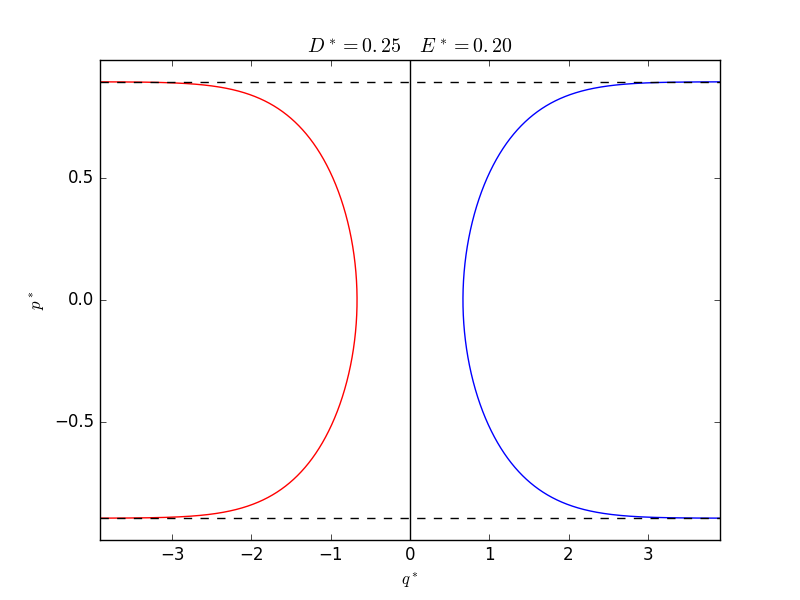
\includegraphics[width=0.45\textwidth]{choque1d/curvas_teo_1.png}}
	\subfigure{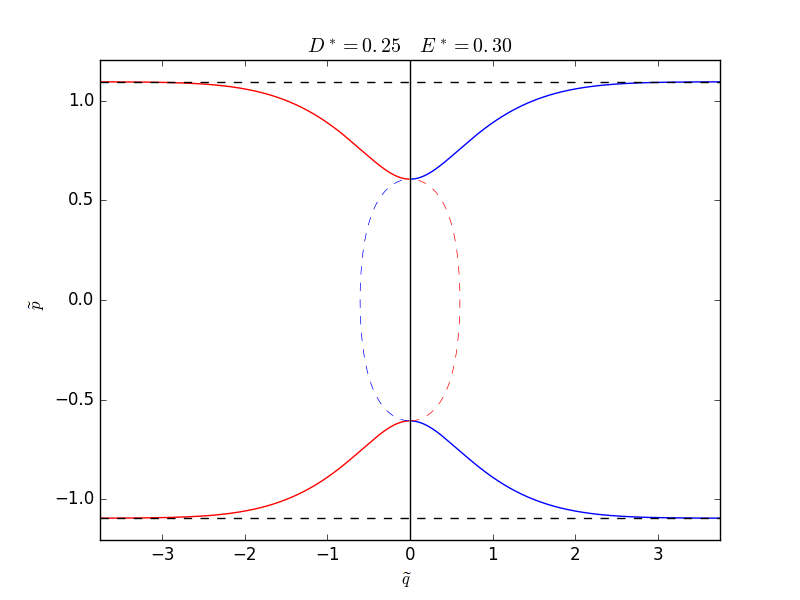
\includegraphics[width=0.45\textwidth]{choque1d/curvas_teo_2.png}}	
	\subfigure{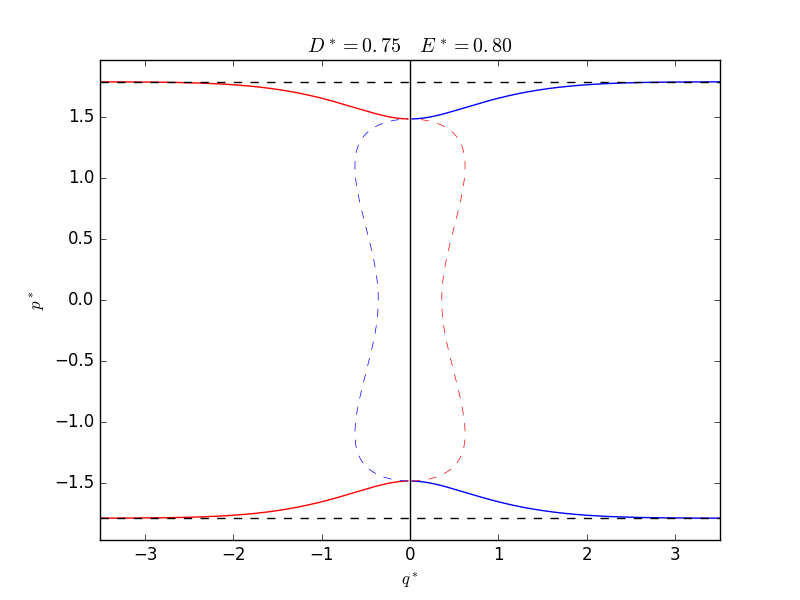
\includegraphics[width=0.45\textwidth]{choque1d/curvas_teo_3.png}}
	\subfigure{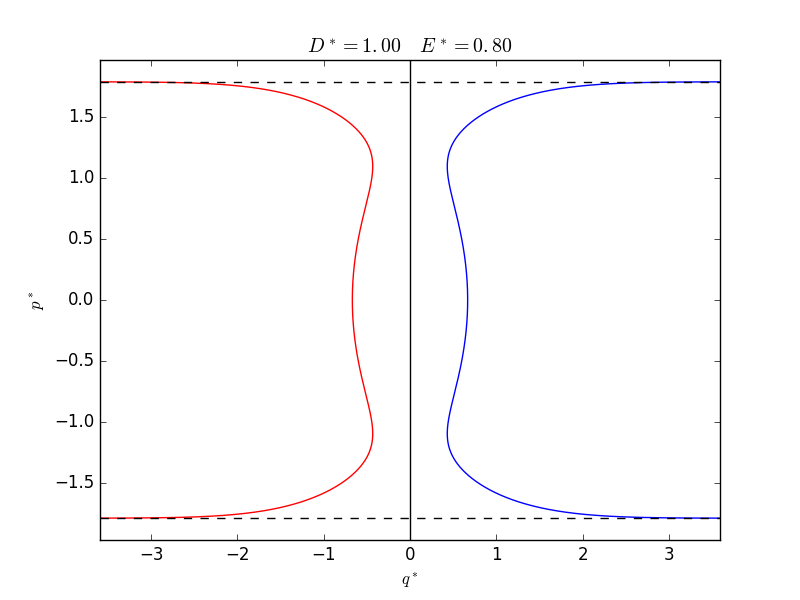
\includegraphics[width=0.45\textwidth]{choque1d/curvas_teo_4.png}}
	\caption{Area de la región excluída en función de $D^*$ obtenida de integrar numéricamente \eqref{eq:area_int_ex}. Para valores altos parece haber una relación lineal entre $A^*$ y $\log D^*$.}
	\label{fig:curvas_teo}
\end{figure}

La existencia de región excluida existe solo para $D^*>1/2$ puede apreciarse para las curvas de doble rebote, que parecen estar circunventando el origen. 
Como dijimos, a medida que $E^*\to E^*_c = (1+\log(2D^*))/2$ estas curvas acercarán sus mínimos al eje $q^*=0$ hasta transformarse en curvas de atraviese.
Es justamente para $E^*\to E^*_c $ por debajo donde los mínimos de $q\geq0$ y $q\leq0$ se conectan, encerrando la región excluída. 
Por lo tanto, la curva $q^{*2}(p^*; E^*=E_c^*)$ define el perímetro de esta región y podemos utilizarla para calcular el área total encerrada según

\begin{align*}
A^* = 2\int_{-\sqrt{p_\infty^2-2}}^{\sqrt{p_\infty^2-2}} q^*(p) dp \Bigg|_{p_\infty^2=4E^*_c}
&= 4\int_{0}^{\sqrt{p_\infty^2-2}} \sqrt{-p^2 - 2\log\left( \frac{p_\infty^2-p^2}{2} + \log(2D^*) \right)} dp \Bigg|_{p_\infty^2=4E^*_c}
\end{align*}

Mediante el cambio de variables $x = (p_\infty^2-p^2)/2$, $dx = -p dp \Rightarrow dp = -dx/\sqrt{p_\infty^2-2x}$ y usando que $p_\infty^2 = 4E^*_c$ y $\log(2D^*) = 2E_c^* - 1$

\begin{equation}{\label{eq:area_int_ex}}
A^* = 4\int_{1}^{2E_c^*} \frac{\sqrt{-4E_c^* + 2x - 2\log(x) + 4E_c^* - 2}}{\sqrt{4E_c^* - 2x}} dx
= 4\int_{1}^{2E_c^*} \frac{\sqrt{x -1 - \log(x)}}{\sqrt{2E_c^* - x}} dx
\end{equation}
donde debemos recordar que $2E_c^* = 1 + \log(2D^*) $ y que $A^*$ es el área reducida, siendo el área total $A = q_op_oA^*$.

Sin embargo, la integral de \eqref{eq:area_int_ex} no puede expresarse como una combinación de funciones conocidas, lo cual nos impide por completo obtener una forma funcional clara.
Aún así, podemos realizar una integración numérica de $A^*$ vía regla de trapecios.
Debemos tener especial cuidado en el extremo superior, donde el integrando diverge.
El resultado de esta integración numérica en un amplio rango de $D^*$ puede apreciarse en la \textbf{Figura \ref{fig:AvsD_teo}}, donde vemos que rápidamente se alcanza una tendencia lineal $A^* \approx \alpha \log(D^*) + \beta$.

\begin{figure}[h]
	\centering
	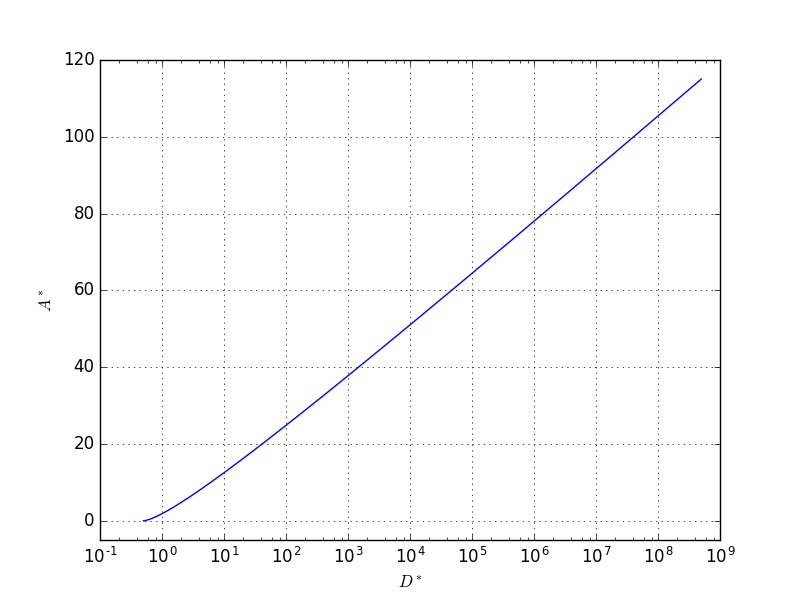
\includegraphics[width=0.8\textwidth]{choque1d/AvsD_solo_teo.png}
	\caption{Area de la región excluída en función de $D^*$ obtenida de integrar numéricamente \eqref{eq:area_int_ex}. Para valores altos parece haber una relación lineal entre $A^*$ y $\log D^*$.}
	\label{fig:AvsD_teo}
\end{figure}

Recordando las propiedades \eqref{eq:props_area_red} que esperabamos de $A^*$, es inmediato de la \textbf{Figura \ref{fig:AvsD_teo}} que $A^*$ es creciente en $D^*$.
La segunda propiedad, sin embargo, no resulta tan evidente. 
Computando la integral \eqref{eq:area_int_ex} para obtener $A^*(1)$, podemos graficar $A^*$ junto con $A^*(1)D^*$ para verificar esta segunda propiedad.
En la \textbf{Figura \ref{fig:AvsD_teo_cota}} podemos apreciar que esta cota se cumple para  $0.5\leq A^*\leq 1$ y $250\leq A^*$, lo cual resulta llamativo.

\begin{figure}[h]
	\centering
	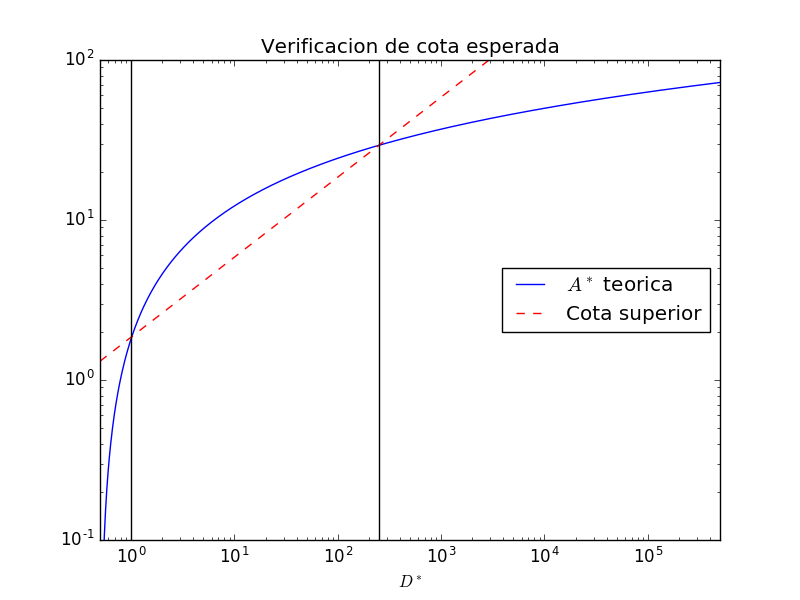
\includegraphics[width=0.8\textwidth]{choque1d/AvsD_cota_teo.png}
	\caption{Area de la región excluída en función de $D^*$ obtenida de integrar numéricamente \eqref{eq:area_int_ex}. Para valores altos parece haber una relación lineal entre $A^*$ y $\log D^*$.}
	\label{fig:AvsD_teo_cota}
\end{figure}

Es importante aclarar, de todos modos, que la cota superior para $A^*$ era una propiedad \textit{deseable}, pero no realmente necesaria.
Que no se cumpla implica que un aumento en $p_o$ puede generar una reducción en el área de la región excluída, pero esto no resulta particularmente problemático.
La propiedad más relevante del potencial de Pauli es la existencia de un área excluída y la capacidad de poder adaptar $D^*$ para que este área sea la buscada, lo cual ciertamente se cumple.

Más adelante retomaremos este análisis del espacio de fases desde un punto de vista computacional, simulando el choque y confirmando nuestros resultados con esta sección.




\subsection{Estudio numérico del espacio de fases}{\label{sec:num_choque_1d}}

Como dijimos, las curvas $q(p)$ del diagrama de fases mantienen el Hamiltoneano $H(q,p)$ constante.
A la hora de simular, un método que conserve la energía del sistema arrojará estas curvas $q(p)$ inmediatamente.

Una simulación de dinámica molecular evolucionando el sistema con las ecuaciones de Hamilton con un integrador simpléctico nos asegura esto más, por lo que resulta mucho más natural 
que otros métodos donde la energía fluctua (como Metropolis-Montecarlo).


\subsubsection{Implementación de integradores}{\label{sec:imp_integs}}

Según lo que discutimos en la sección \ref{sec:int_simpl}, dado que el Hamiltoniano \eqref{eq:hamiltoniano_1D} es no separable, no disponemos de integradores simplécticos y explícitos.
Con el objetivo de comparar, decidimos implementar 2 integradores no simplécticos pero explícitos y un integrador simpléctico pero no explícito.

Además, para simplificar la notación definimos \[y = \binom{p}{q} \qquad J = \begin{pmatrix}
0 & \mathbb{I} \\
-\mathbb{I} & 0
\end{pmatrix}
\]

Los integradores implementados son Euler, un Runge-Kutta de orden 2 (RK2) y MidPoint Rule (MPR).
Los esquemas pueden apreciarse junto con su información relevante en la \textbf{Tabla \ref{tab:integradores}}. 
La simplecticidad de MPR fue probada en \ref{sec:int_simpl} mientras que la no simplecticidad de Euler y RK2 se encuentra en el apéndice \ref{sec:no_simp}.

\begin{table}[h]
	\centering
	\begin{tabular}{|c|c|c|c|c|}
		\hline
		\textbf{Integrador} & \textbf{Esquema} & \textbf{Orden} & \textbf{¿Explícito?} & \textbf{¿Simpléctico?} \\ \hline
		Euler & $ y_{n+1} = y_n + hJ^{-1}\nabla H(y_n)$ & $1$ & Si & No \\ \hline
		Runge-Kutta 2 & $y_{n+1} = y_n + hJ^{-1}\nabla H\left(y_n+\frac{h}{2}\nabla H(y_n) \right)$ & $2$ & Si & No \\ \hline
		Midpoint Rule & $y_{n+1} = y_n +  hJ^{-1}\nabla H\left(\frac{y_n+y_{n+1}}{2} \right)$ & $2$ & No & Si \\ \hline
	\end{tabular}
	\caption{Comparación de los integradores utilizados}
	\label{tab:integradores}
\end{table}

Dado que no es explícito, para el integrador MPR implementamos además un método de punto fijo para poder resolver cada paso.
Sumando $y_n$ a cada lado del esquema MPR y dividiendo por 2, podemos redefinir $Z = \frac{y_n+y_{n+1}}{2}$ tal que
\[ Z = y_n + \frac{h}{2}J\nabla H(Z) \equiv F(Z) \]
y resolver esta ecuación de punto fijo con parámetro conocido $\mathbf{y}_n$ en \textit{cada iteración} evaluando múltiples veces $F(Z)$.
En principio, puede probarse que $|DF(Z)|<1$ (punto fijo converge) para $h$ suficientemente chico dado que el Hessiano del potencial de Pauli está acotado (es gaussiano).
Sin embargo, la cota para $h$ dependerá de los parámetros $p_o$, $q_o$ y $D$ e incluso podría depender del número de partículas $N$ del sistema.
Por lo tanto, en principio nos conformaremos con saber que tal $h$ existe e intentar encontrarlo según la situación.

En lo que sigue, siempre resolvimos el problema de punto fijo $Z = F(Z)$ utilizando $k=5$ iteraciones, al notar que valores más altos de $k$ no mejoraban apreciablemente la convergencia.
Cabe aclarar, sin embargo, que sistemas con más partículas pueden a priori exigir valores mayores de $k$.

\subsubsection{Conservación de la energía}

A modo de comparación, corrimos una simulaciones del choque de 2 partículas en 1D, muestreando el Hamiltoniano (de ahora en más, la energía) a lo largo del recorrido.
Consistentemente con lo que vimos en la sección \ref{sec:teo_fases}, durante el choque de 2 partículas pueden darse 2 situaciones: rebote o atraviese, dependiendo del valor inicial del Hamiltoniano $E$ y el valor de $D$.

Dado que en general nos interesa trabajar con potenciales de Pauli con región excluida, configuramos el potencial de Pauli con $D = 10000$ y aprovechamos la adimensionalización para tomar $qo = 1 = po = m$ tal que $D^*=D>1/2$.
En este caso particular, analizaremos un atravesado.
El sistema comienza con una de las partículas en el origen con impulso nulo (en la posición $(0, 0)$ del espacio de fases) y otra a distancia $6$ e impulso $-4$ (en el $(6, -4)$).

A modo de ejemplo y para visualizar el problema, en la \textbf{Figura \ref{fig:energ_choq}} puede apreciarse la energía durante un choque para paso temporal $h=0.01$.
Es interesante notar que RK2 tiende a aumentar $E$ mientras que Euler tiende a disminuirla; está clara la mayor efectividad de MPR.

\begin{figure}[h]
	\centering
	\subfigure[Euler]{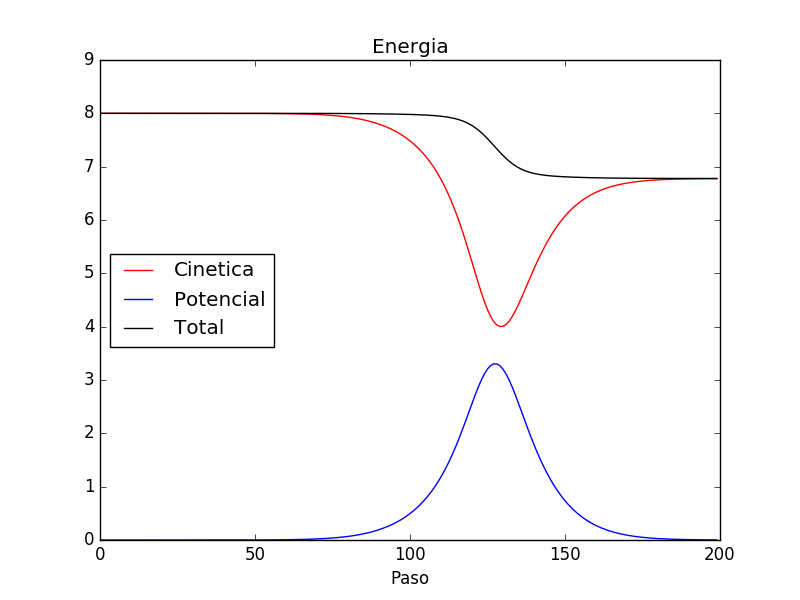
\includegraphics[trim = 20mm 0mm 15mm 10mm, clip, width=0.32\columnwidth]{choque1d/energia_euler_0,01.png}}
	\subfigure[Runge-Kutta 2]{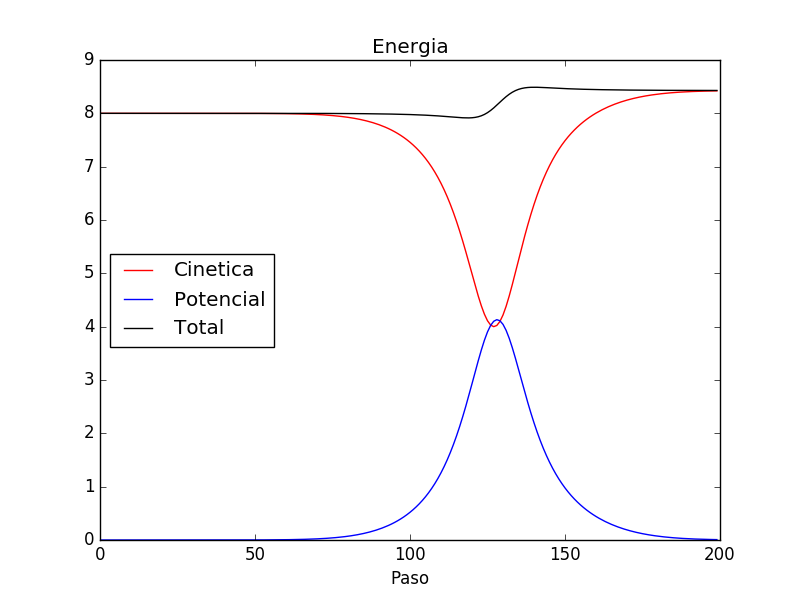
\includegraphics[trim = 20mm 0mm 15mm 10mm, clip, width=0.32\columnwidth]{choque1d/energia_rk2_0,01.png}}
	\subfigure[Midpoint Rule]{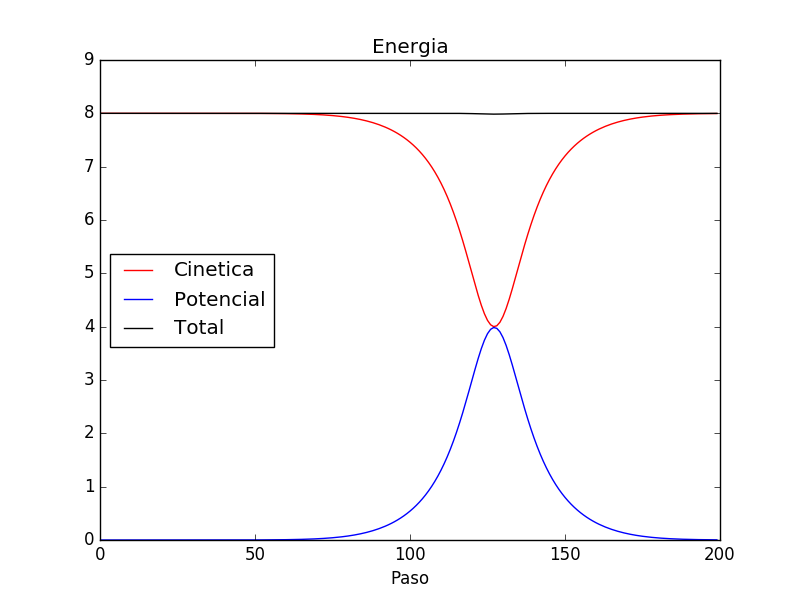
\includegraphics[trim = 20mm 0mm 15mm 10mm, clip, width=0.32\columnwidth]{choque1d/energia_mpr_0,01.png}}
	\caption{Energía durante un choque para un potencial de Pauli con $D = 10000$ y $qo = 1 = po = m$. La trayectoria comenzó en el $(q, p) = (6, -4)$, integrada con paso temporal $h=0.01$}
	\label{fig:energ_choq}
\end{figure}

Realizamos estos choques para distintos valores de $h$ (y las mismas condiciones iniciales) y analizamos la fluctuación relativa de energía (siempre positiva para este hamiltoneano).
Los resultados pueden apreciarse en la \textbf{Figura \ref{fig:flucvsh}}, donde se confirma la clara superioridad de MPR a la hora de conservar la energía.
Esto último resulta a priori esperable dado que MPR es un integrador simpléctico; no obstante, al ser resuelta la ecuación con un método de punto fijo, esto pudo haber dejado de ser cierto.

\begin{figure}[h]
	\centering
	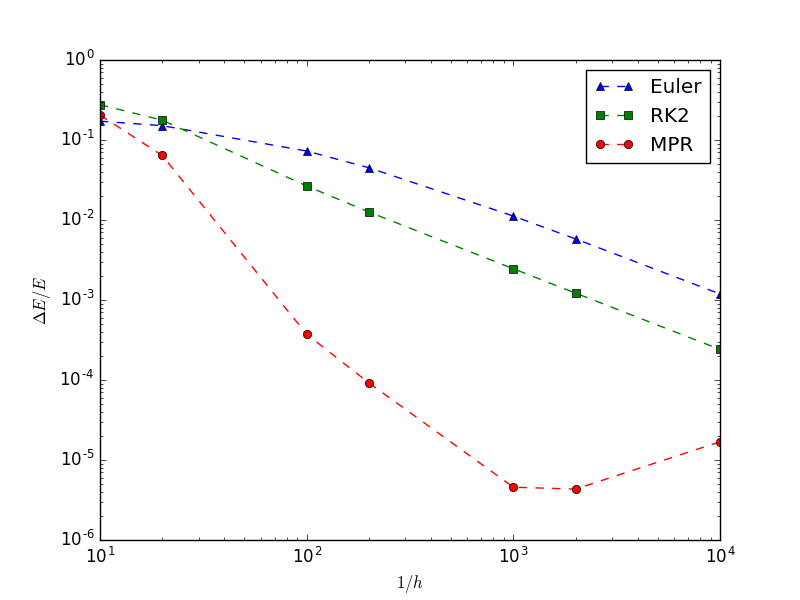
\includegraphics[trim = 0mm 0mm 15mm 10mm, clip, width=0.6\columnwidth]{choque1d/fluct_vs_h.png}
	\caption{Fluctuaciones de energía en función de paso temporal para distintos integradores.}
	\label{fig:flucvsh}
\end{figure}

\subsubsection{Primer diagrama de fases}

Como dijimos, al ser un sistema unidimensional $(q,p)$, el diagrama de fases queda definido univocamente por $H(q,p)\equiv E = \text{cte}$.
Por lo tanto, la conservación de la energía por parte de los integradores resulta suficiente para obtener estas curvas $q(p)$ y así construir el diagrama.
Con este objetivo, configuramos el sistema inicialmente con una partícula en el $(0,0)$ y la otra en un valor $(q_i, p_i)$.
Luego, evolucionamos el sistema muestreando los valores de $q = q_1 - q_2$, $p = p_1 - p_2$.
Decidimos utilizar MPR para la evolución, dado que para $h=10^{-3}$ se tenía la mayor estabilidad de la energía y un tiempo de cómputo accesible.

Tomamos entonces un rango de condiciones iniciales $(q_i,p_i)=(5,p)$ con $p\in [-6,0]$ y analizamos las curvas $q(p)$ resultantes, sabiendo que el cambio de $p$ se traduce en un cambio de $E$. 
Mantuvimos $q_i$ fijo dado que así emulabamos una colisión desde el infinito, dado que $V_P(5,p)\leq 4\times10^{-6}V_P(0,0) = 4\times10^{-6}D$ que podemos considerar nulo.
Utilizamos los mismos parámetros para el potencial de Pauli ($D=10000$, $m=1=p_o=q_o$) por consistencia.
En la \text{Figura \ref{fig:ej_diag_fases}} podemos ver estas curvas superpuestas en nuestro primer diagrama de fases.

\begin{figure}[h]
	\centering
	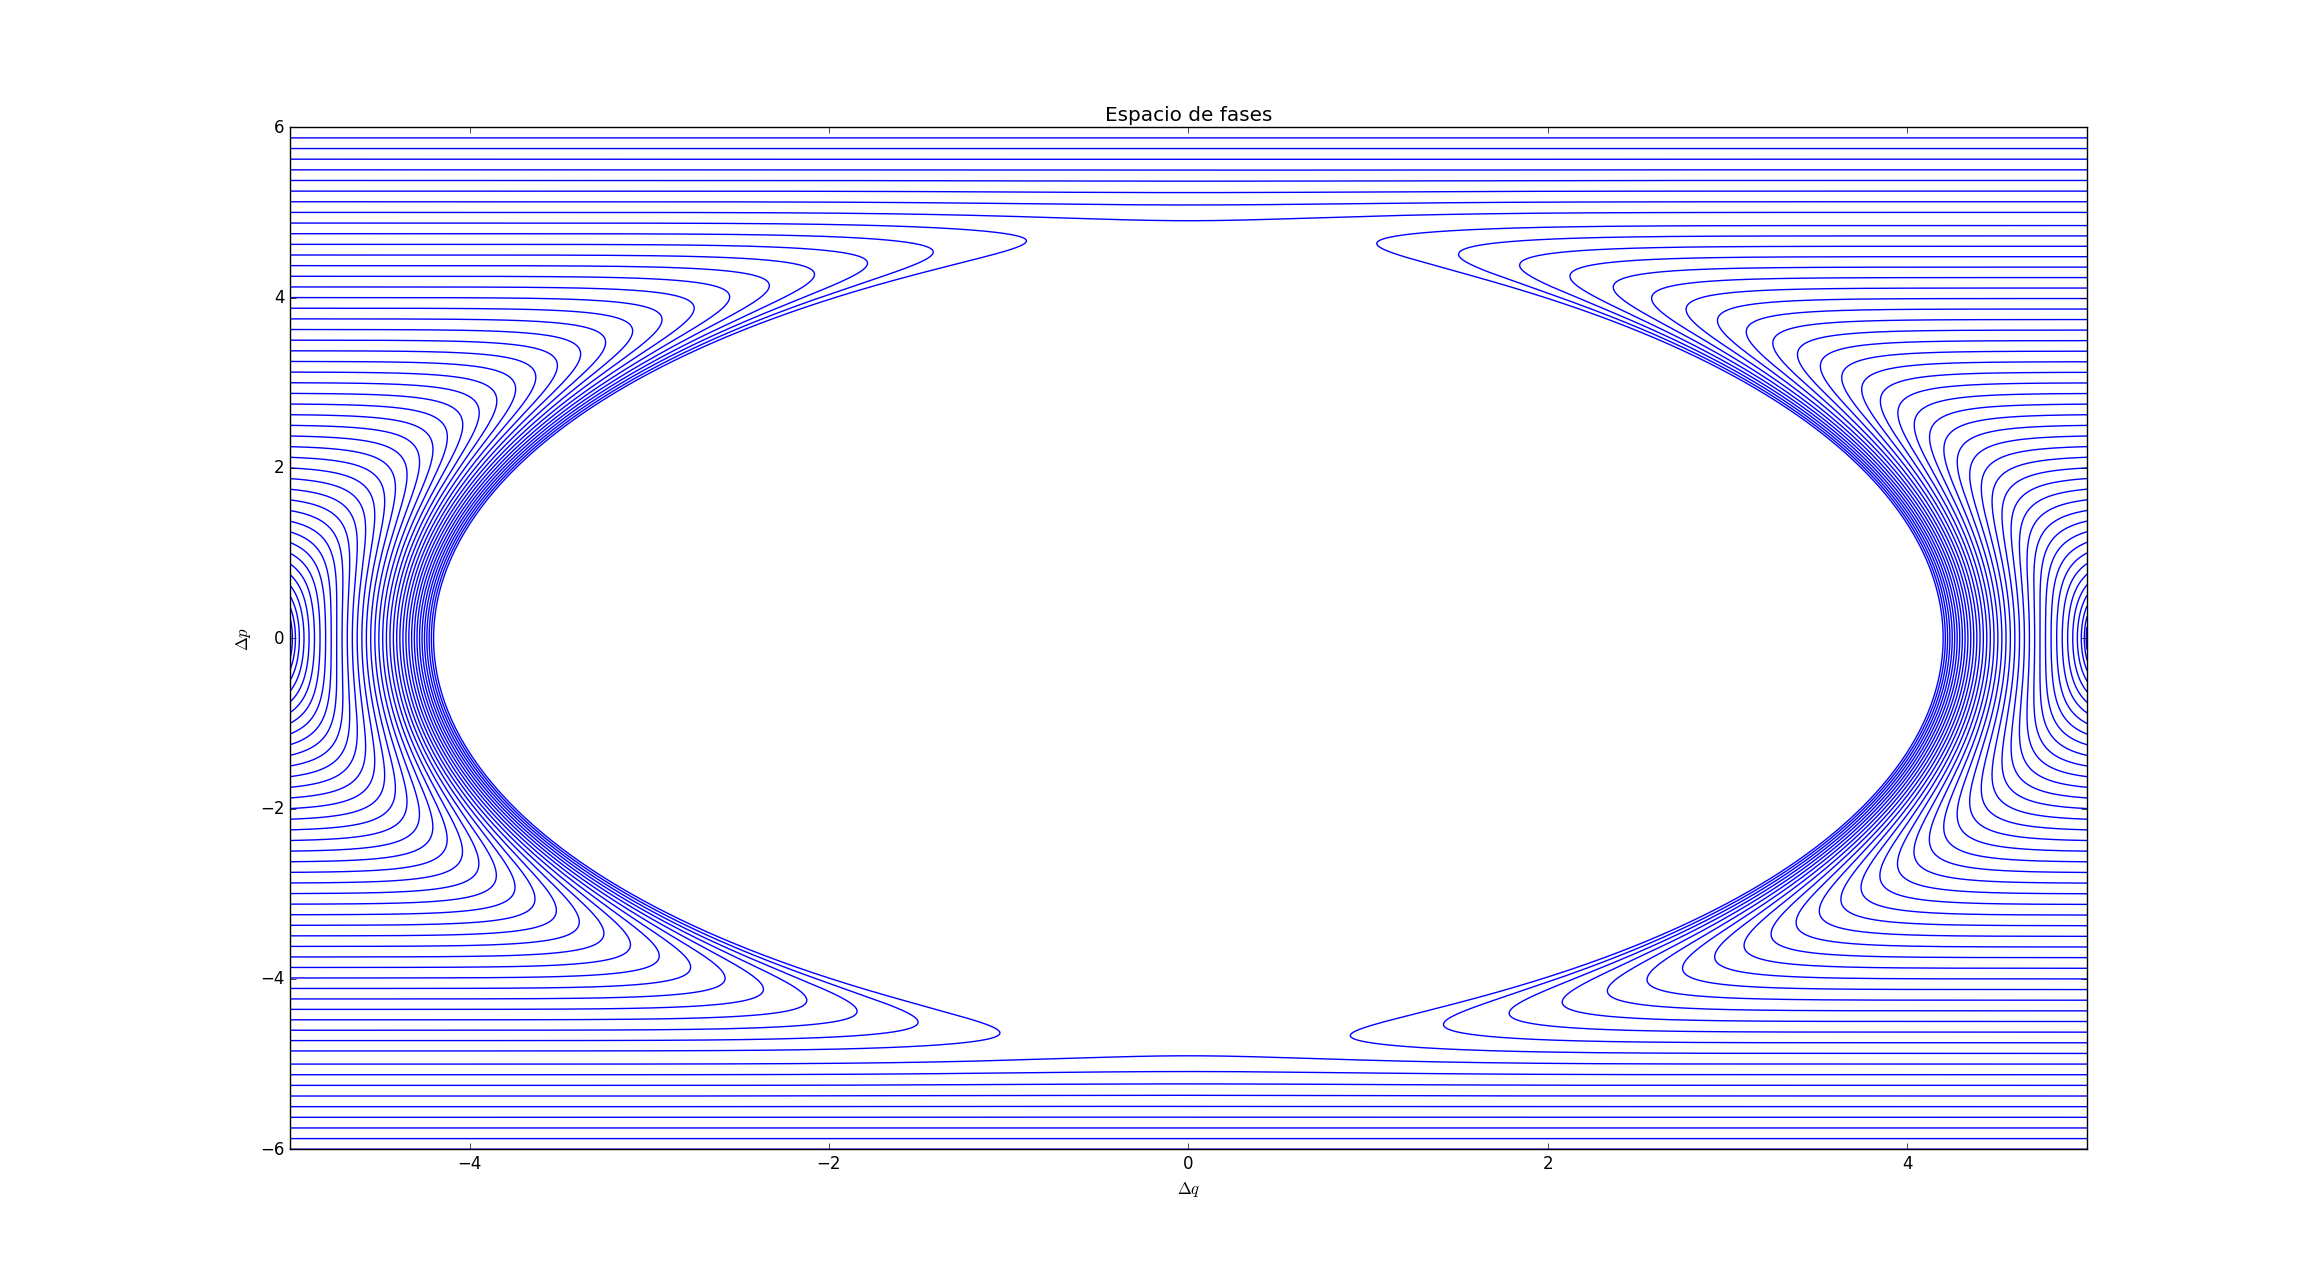
\includegraphics[width=0.9\textwidth]{choque1d/fases.png}
	\caption{Diagrama de fases para $D=10000$, $m=1=p_o=q_o$ y $h=10^{-3}$. Además de la zona inaccesible, se evidencian las curvas de rebote y atraviese según lo previsto en \ref{sec:teo_fases}}
	\label{fig:ej_diag_fases}
\end{figure}

Resulta fundamental notar que el diagrama se compone de dos tipos de curva: rebotes y atravieses.
En particular, los rebotes tienen dos puntos de máxima cercanía, en perfecta concordancia con lo analizado en \ref{sec:teo_fases} dado que tenemos $D^*=10^4>1/2$.
Incluso puede verse que la transición de rebote a atraviese ocurre para $4.625\leq p_i\leq4.75$, consistente con
\[ E_c = \frac{p_i^2}{4} = \frac{1}{2}\left( 1 + \log(2D) \right) \approx 5.45 \Longrightarrow p_i \approx 4.67 \]

Veremos en la sección \ref{sec:area_ex_comp} que no solo se verifica esto sino también el área total excluída, cuyo cómputo tiene sus propias complicaciones.


\subsubsection{Teorema de Liouville y volumen de fases}

Como discutimos en la seccion \ref{sec:trans_simp}, la simplecticidad de las ecuaciones de Hamilton asegura no solo la conservación de la energía, sino la conservación del volumen orientado \eqref{eq:area_orien_simp}.
Esto conlleva, en otras cosas, al Teorema de Liouville y la conservación del volumen de fases.
La evolución de una dada región de condiciones iniciales en el espacio de fases preserva su volumen total.

Por lo tanto, otro criterio para calificar la efectividad de los integradores es la conservación del volumen de fases a lo largo de la evolución.
Para esto, realizamos una simulación tomando un conjunto de valores iniciales $(q_i, p_i)$ y evolucionándolos en paralelamente en el tiempo.
En cada paso, asumiendo que cada punto era una elipse rígida de área definida, calculamos el volumen del conjunto de puntos como la suma de sus volumenes individuales.

Hicimos esto para curvas de rebote (doble) con 81 condiciones iniciales en un cuadrado de $0.04\times0.04$ alrededor del $(6, -4)$ y los mismos parámetros de antes para Pauli.
Tomamos estas elipses suficientemente grandes como para cubrir completamente este cuadrado inicial, por lo que hubo considerable superposición de volumenes.
Los resultados pueden apreciarse en la \textbf{Figura \ref{fig:vol_fas}}.

\begin{figure}[h]
	\centering
	\subfigure[h = 0.01]{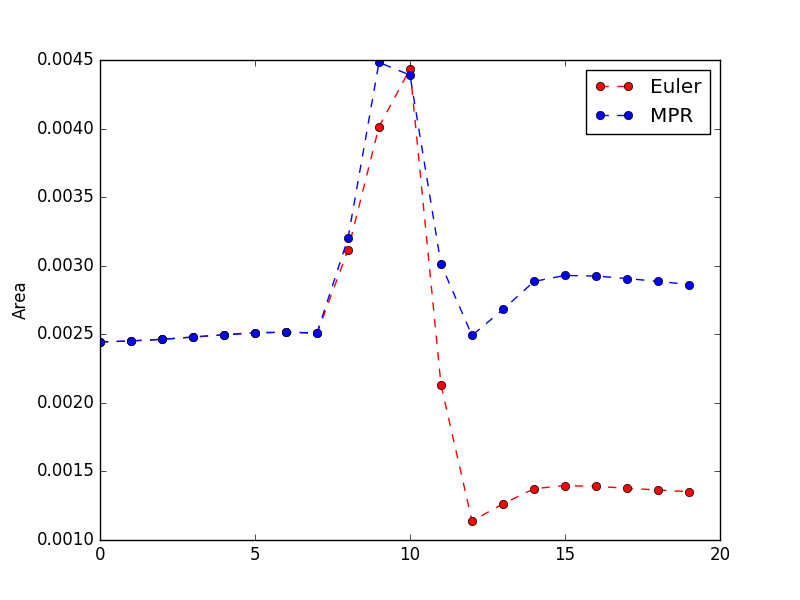
\includegraphics[trim = 0mm 0mm 15mm 10mm, clip, width=0.32\columnwidth]{choque1d/vol_fas_0,01.png}}
	\subfigure[h = 0.005]{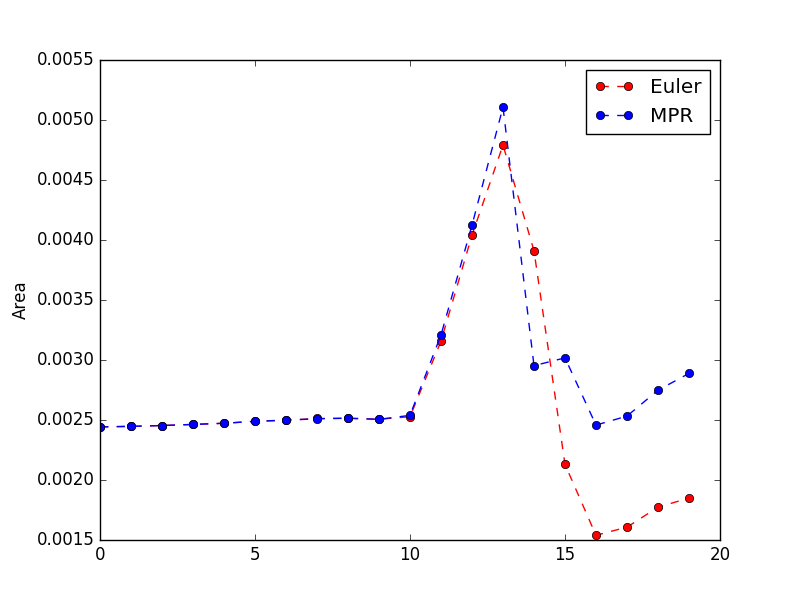
\includegraphics[trim = 0mm 0mm 15mm 10mm, clip, width=0.32\columnwidth]{choque1d/vol_fas_0,005.png}}
	\subfigure[h = 0.001]{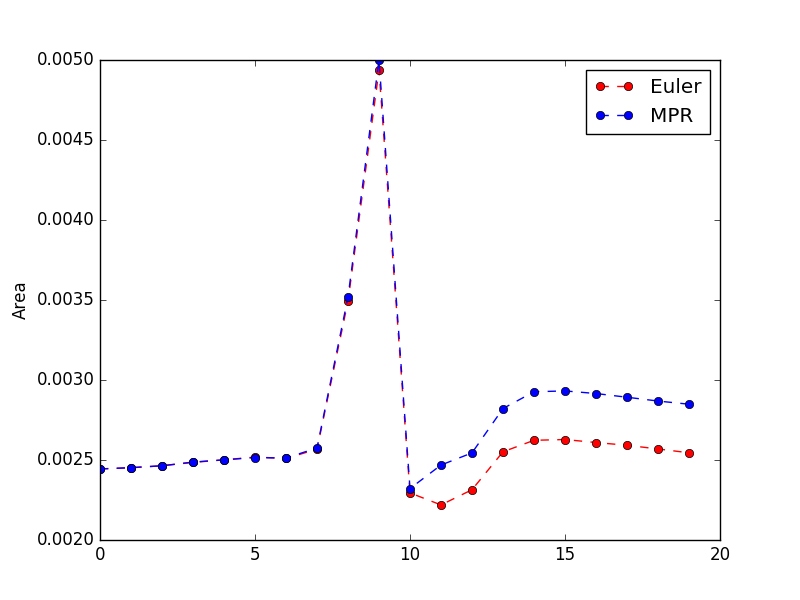
\includegraphics[trim = 0mm 0mm 15mm 10mm, clip, width=0.32\columnwidth]{choque1d/vol_fas_0,001.png}}
	\caption{Volumen de un conjunto de puntos a lo largo de una curva de rebote. El pico corresponde al momento de máxima interacción.}
	\label{fig:vol_fas}
\end{figure}

Lo primero que podemos notar es la existencia de un pico, que corresponde los instantes de mayor interacción entre las partículas.
Sin embargo, es importante notar que luego de ello los volumenes recuperan su valor inicial.
Esto es un buen indicio y ocurre para $h=10^{-3}$ para ambos integradores, pero solo para el MPR en los otros 2 casos.
En un tercer caso con $h=0.1$ que omitimos, ninguno de los 2 métodos cumplía esto.

Para comprender este pico, nos basta analizar la \textbf{Figura \ref{fig:ej_diag_fases}} y notar que entre rebotes se da la mayor interacción.
En esta región, las curvas de nivel se comprimen, aumentando considerablemente su densidad. 
Es por esto que nuestro conjunto de puntos (inicialmente dispuestos en un cuadrado) tiende a alinearse en una figura predominantemente unidimensional, donde resulta claro que la estimación del área 
como superposición de elipses rígidas no es apropiada, sobreestimando el área.

Sin embargo, nos resulta suficiente notar que el volumen de fases se conserva luego de cada choque, donde vemos nuevamente que el integrador MPR tiene una mayor robustez, 
manteniendo las propiedades de una evolución simpléctica para valores de $h$ mayores comparado a Euler.


\subsection{Area excluída}{\label{sec:area_ex_comp}}

Con el objetivo de obtener $A^*(D^*)$ de la simulación, nuevamente tomaremos $q_o = p_o = m = 1$ de forma que $D^* = D$ y $A=A^*$.
De esta manera, solo es necesario calcular el área de la región excluída.
Para esto, sin embargo, es necesario identificar la curva $C$ de rebote que define esta región.
Para simplificar la notación, definimos la curva $C(q_i,p_i)$ como la curva de energía constante $H(q_i,p_i)$; la curva sobre la que evoluciona el sistema.
De esta manera, la curva $C(q_i,p_i)$ puede pensarse como la que describe el sistema con condiciones iniciales $(q_i,p_i)$.

Con esto en mente, corremos simulaciones que muestreen las curvas $C$ para encontrar el mayor valor de $p_i$ tal que $C(q_i, p_i)$ es un rebote.
Como antes, fijaremos $q_i=5$ pero no discriminaremos entre rebotes simples y dobles, dado que moveremos $D^*$ por ensima y por debajo de $1/2$.
Realizamos esta búsqueda en forma binaria, tomando un $p_{max}$ que cumpla que $C(q_i, p_{max})$ sea un atraviese, sabiendo que $C(q_i, 0)$ \textbf{\textit{siempre}} es un rebote.
Obtenemos el $p_{max}$ tomando un valor inicial $p_max = -3$ y duplicándolo hasta obtener un atraviese.
Con estos 2 valores de impulso, iteramos la busqueda binaria hasta que $|p_{max}-p_{min}|\leq tol$.
El valor de $tol$ resulta arbitrario, por lo que tomamos uno dependiente de $D^*$ según $tol \sim \sqrt{D^*}\times 10^{-4}$, pues consideramos que para $D^*=10^4$ 
una $tol = 10^{-2}$ resultaba apropiada y lo extendimos usando la cota $A^*\leq \sqrt{D^*}$.
El paso temporal fue $h=10^{-3}$ para $D\leq 1000$, $h=5\times10^{-3}$ para $5000\leq D\leq 50000$ y $h=10^{-4}$ para $D\geq 100000$.

Los resultados pueden apreciarse en la \textbf{Figura \ref{fig:AvsD}} junto con algunos ejemplos del espacio de fases (con mayor definición cerca de la región de interés).
En la misma figura está nuevamente el gráfico del área según el cálculo teórico, que resulta concordante.
La primera observación es que $A=0$ para $D\leq 0.5$, donde las curvas de rebote son cóncavas (rebote simple) para $q\approx 0$ a diferencia del caso $D\geq 0.5$ donde son convexas 
(para rebote doble, como en el ejemplo de la \textbf{Figura \ref{fig:ej_fases}}). 
De hecho, puede apreciarse que para $D=0.5$, las curvas son prácticamente verticales, marcando este cambio de convexidad.

\begin{figure}[H]
	\centering
	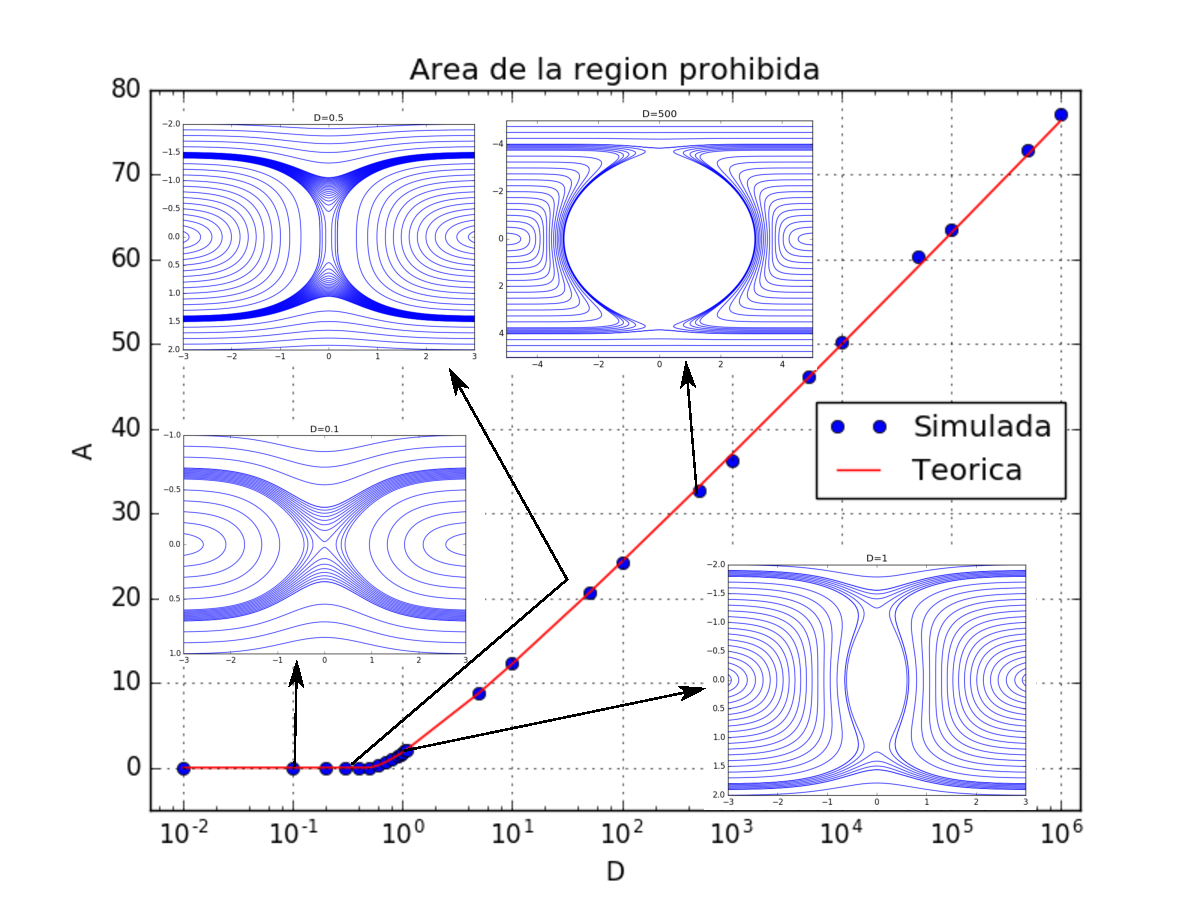
\includegraphics[trim = 0mm 0mm 15mm 10mm, clip, width=\columnwidth]{choque1d/AvsD_full_teo.pdf}
	\caption{Area prohibida en función de intensidad de potencial junto con algunos de los espacios de fase asociados. 
	Tenemos $A^*=0$ para $D\leq 0.5$ y $A\sim \log{D^*}$ para $D\geq 1$ en perfecto acuerdo con la formulación teórica.}
	\label{fig:AvsD}
\end{figure}

Paralelamente, podemos graficar los valores de $p_b$ obtenidos; tenemos un rebote para $p\leq p_b$ y un atraviese para $p>p_b$.
En particular, es $E_c = p_b^2/4$, por lo que según vimos en \ref{sec:teo_fases} tiene forma de función partida.
Para $D^*\leq 0.5$, es $p_b=2\sqrt{D^*}$ y para $D^*>0.5$ $p_b=\sqrt{2(1+\log(2D^*))}$.
La comparación del valor obtenido por la simulación con el teórico se encuentra en la \textbf{Figura \ref{fig:pbvsD}}.
Ambos coinciden dentro del (amplio) rango estudiado.

\begin{figure}[H]
	\centering
	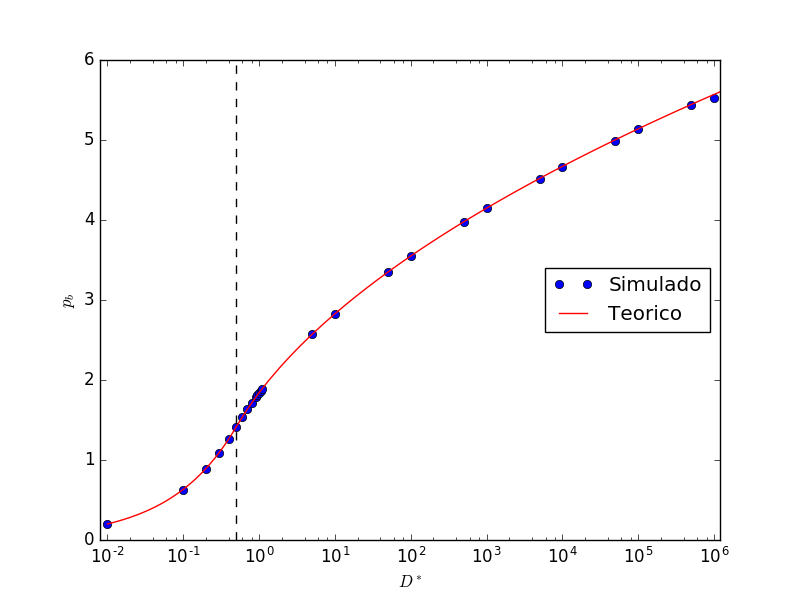
\includegraphics[trim = 0mm 0mm 15mm 10mm, clip, width=0.75\columnwidth]{choque1d/pinfvsD.png}
	\caption{Impulso crítico de transición (en módulo) rebote-atraviese en función de intensidad de potencial junto con el valor teórico, con el que coincide
	correctamente. La linea punteada marca $D^*=1/2$, donde la forma funcional de $p_b$ cambia.}
	\label{fig:pbvsD}
\end{figure}







\newpage

\section{Gas de Pauli}{\label{sec:pauli_gas}}
En esta sección, extenderemos el número de partículas a $N_{part}=1000$, transformando nuestro choque unidimensional en un gas de particulas interactuantes vía potencial
de Pauli: un \textit{gas de Pauli}.
Como dijimos, nuestro objetivo es confirmar si es posible utilizar este potencial para reproducir las distribuciones de un gas de fermiones no interactuantes (o \textit{gas de Fermi}).

El Hamiltoniano de este gas de Pauli será

\begin{equation}{\label{eq:pauli_gas_ham}}
 H(\mathbf{q}_1, ...,\mathbf{q}_N; \mathbf{q}_1,..., \mathbf{q}_N) = \sum_{i=1}^{N} \frac{p_i^2}{2m} + \sum_{i=1}^N\sum_{j=1}^{i-1} De^{-\frac{1}{2}s_{ij}^2}
 \quad \text{ con } \quad s_{ij}^2 = \frac{|\mathbf{q}_i-\mathbf{q}_j|^2}{q_o^2} + \frac{|\mathbf{p}_i-\mathbf{p}_j|^2}{p_o^2}
\end{equation}

\subsection{Método de simulación}

Con esto en mente, comenzamos extendiendo los algoritmos de la Sección \ref{sec:num_choque_1d} para un sistema de $N$ partículas en 3 dimensiones.
En particular, usamos MPR con el método de punto fijo de $k=5$ iteraciones para resolver la ecuación implícita que dicta la evolución temporal del sistema.

Buscamos estimar preliminarmente los tiempos, variando la cantidad de partículas $N$ y analizando el tiempo $\tau_{1000}$ que tardaba el programa en avanzar
$1000$ pasos con $h=5\times10^{-4}$.
Los resultados fueron desalentadores y se encuentran en la \textbf{Figura \ref{}}, donde podemos ver la esperada tendencia cuadrática con 
$\tau_{1000} \approx 0.9753\mu s N^{1.988}$. 
Esto implica que para $N_{part}=1000$, el programa tardaba $\sim0.86s$ por paso, lo cual resulta simplemente prohibitivo al exigir días de simulación para termalizar el sistema.

\begin{figure}[h]
	\centering
	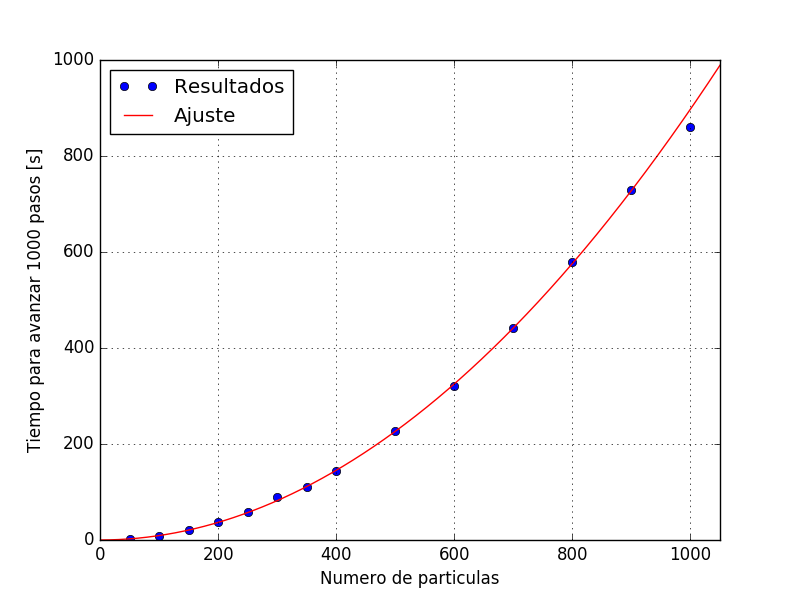
\includegraphics[width=0.6\textwidth]{pauli_gas/tiempo_vs_N.png}
	\caption{Tiempo necesario para avanzar un sistema de $N$ partículas en 1000 pasos con $h=5\times10^{-4}$. 
	La tendencia es cuadrática y exige $\sim0.86s$ por paso para $N=1000$, lo cual es prohibitivo.}
	\label{fig:ej_diag_fases}
\end{figure}

Esto no debería sorprendernos, dado que el método MPR resuelto por punto fijo exige el cómputo de fuerzas $k=5$ veces en total, más del doble de lo exigido por métodos clásicos como Velocity-Verlet.
Además, cabe aclarar que deben computarse las \textit{güerzas} en adición a las fuerzas habituales.
Por último, se suman las complejidades propias del potencial en si, que exige no solo el cálculo de la distancia en el espacio sino también el de la distancia en impulsos y de la necesidad 
de computar una exponencial, siempre más costoso computacionalmente que cualquier potencia. 

Incluso este $k=5$ resultaba insuficiente a medida que $N$ aumentaba, lo cual es razonable si consideramos que la velocidad de convergencia del método de punto fijo (sección \ref{sec:imp_integs})
depende de $N$ a través de $\nabla^2H$.
De hecho, debió tomarse $h=5\times10^{-4}$ (la mitad que en las simulaciones del choque 1D) para mantener la estabilidad del algoritmo durante estras pruebas, lo cual indirectamente exige una 
mayor cantidad de pasos para alcanzar un equilibrio y muestrear propiedades del sistema. 

Frente a esto, consideramos más apropiado el uso del método de Metropolis-Montecarlo descripto en \ref{sec:alg_mm} para el Hamiltoniano \eqref{eq:pauli_gas_ham}.
La principal ventaja de este método es que resulta lineal en $N$ dado que el cómputo de $\Delta E$ al modificar la $k$-esima partícula es

\begin{equation}{\label{eq:delta_E}}
 \Delta E =  \frac{|\mathbf{p}_k + \Delta \mathbf{p}|^2}{2m} - \frac{p_k^2}{2m} + \sum_{i=1, i\neq k}^N D\left( e^{-\frac{1}{2}s_{ik}^{'2}}-e^{-\frac{1}{2}s_{ik}^2}  \right)
\end{equation}

Sin embargo, aún avanzando $N$ pasos (en promedio, un intento de movimiento por partícula) este método tardaba aproximadamente $\tau_N = 0.4s$; menos de la mitad.
Esto sumado a la facilidad para controlar la temperatura (dado que nos interesa un sistema NVT), inclinó la balanza en pos de este método.

En lo que sigue, utilizamos el método de Metropolis-Montecarlo para simular una caja de lado $L$ (y volumen $V=L^3$) con $N$ partículas interactuando mediante un potencial de Pauli $V_P$.
Tomamos valores de $\Delta q$ y $\Delta p$ que nos aseguren una aceptación entre $30\%$ y $60\%$.
Estos $\Delta q$ y $\Delta p$ resultan dependientes de la temperatura $T$, la densidad $\rho = N/V = N/L^3$ e incluso de los propios parámetros del Hamiltoniano.
La forma general de estas variaciones fue entonces $\Delta x = x_o f_x(T, \rho, D^*)$  con $x=q,p$.

Además, impusimos una distancia de corte en el espacio de fases $s_{cut}^2=10$ tal que $V_P=0$ si $s_{ij}\geq s_{cut}$.
Esto lo logramos mediante un \textit{shift} del potencial
\[ V_P(s_{ij}^2) = \left\{\begin{matrix} D(e^{-\frac{1}{2}s_{ij}^2}-e^{-\frac{1}{2}s_{cut}^2}) & \text{si } s_{ij}\leq s_{cut} \\ 0 & \text{si } s_{ij}\geq s_{cut} \end{matrix}\right. \]
donde $e^{-\frac{1}{2}s_{cut}^2}\approx 6.7\times10^{-3}\sim 1\%$ del máximo de interacción para $s_{cut}^2=10$.

Tomamos un sistema con condiciones de contorno periódicas (PBC) y utilizamos el criterio de mínima imagen, para lo cual resultaba necesario que el tamaño $L$ de la caja cumpla
\[ L >2 s_{cut}q_o \approx 6.32q_o \]
de forma tal que no sea posible la interacción con más de una imagen simultaneamente. 

En lo que sigue, analizaremos propiedades de un gas de Pauli bajo dos conjuntos de parámetros habitualmente utilizados en la literatura para Pauli.
En ambos casos, tomaremos una masa $m=100m_p$ con $m_p=938MeV/c^2$ la masa del protón; un elección arbitraria y, en el fondo, no más que una variación del $D^*$.

El primero de estos conjuntos de parámetros corresponde a Dorso \textit{et al} con
\begin{equation}{\label{eq:params_dorso}}
 \begin{matrix}
  p_o = 2.067 MeV\times 10^{-22}s/fm (= 61.969 MeV/c) & q_o = 6 fm\\
  D = \left(\frac{\hbar}{q_op_o}\right)^3 34.32MeV = \left(\frac{1}{1.88}\right)^3 34.32MeV = 5.165MeV & D^* = 126.16
 \end{matrix}
\end{equation}
y el segundo a Maruyama \textit{et al}
\begin{equation}{\label{eq:params_maruyama}}
 \begin{matrix}
  p_o = 120 MeV/c & q_o = 1.644 fm\\
  D = \left(\frac{\hbar}{q_op_o}\right)^3 207MeV = 207MeV & D^* = 1348.375
 \end{matrix}
\end{equation}

En comparación con \eqref{eq:params_dorso}, los parámetros de \eqref{eq:params_maruyama} generan un potencial de mucho mayor intensidad pero con un alcance mucho mayor en $p$
respecto a su alcance en $q$.
Además, tiene un $D^*$ casi 11 veces mayor, pero tiene un área excluída muy similar
\[ A_M\sim 45\hbar \qquad \text{ vs } \qquad  A_D\sim 28\times1.88\hbar \sim 52\hbar\]
Cualquier diferencia entre ambos, entonces, se deberá a cuestiones morfológicas del área excluída definidas por sus $D^*$ tan distintos.
El resto serán cuestiones de escala definidas por $q_o$ y $p_o$.

Analizamos estos parámetros para 3 densidades distintas, pero dado que el $q_o$ de \eqref{eq:params_dorso} resulta casi 4 veces mayor al de \eqref{eq:params_maruyama}, decidimos mantener
constantes las \textit{densidades reducidas} $\rho^* = q_o^3\rho$.
Elegimos entonces $\rho_o^* = (3/2)^3 = 3.375 $, $\rho_1^* = 1 $ y $\rho_2^* = (1/2)^3 = 0.125 $ representando densidades altas, intermedias y bajas, respectivamente.
Enfriamos estos sistemas desde una $T$ inicial alta (dependiente de $p_o$) donde esperabamos que el sistema se comporte como un gas ideal y enfriabamos sucesivamente para observar los
efectos termodinámicos del potencial de Pauli.

Finalmente, hicimos simulaciones similares para un gas interactuando mediante un potencial de Lennard-Jones (LJ)
\[ V_{LJ}(r) = \varepsilon\left( \left( \frac{\sigma}{r} \right)^{12} - \left( \frac{\sigma}{r} \right)^6 \right) \]
cuya única dependencia proviene de 2 parámetros $\sigma$ y $\varepsilon$, lo cual nos permite facilmente trabajar en unidades reducidas donde $\sigma=1=\varepsilon=m$.
Analogamente, analizaremos las densidades $\rho_{LJ,o}^* = 2.9$, $\rho_{LJ,1}^* = 1.05$ y $\rho_{LJ,2}^* = 0.4$ representando densidades altas, intermedias y bajas, respectivamente.

Elegimos estas densidades en base al conocido diagrama de fases del potencial de Lennard-Jones, que nos aseguran que corresponden a gas+líquido, líquido+sólido y sólido.

\begin{figure}[h]
	\centering
	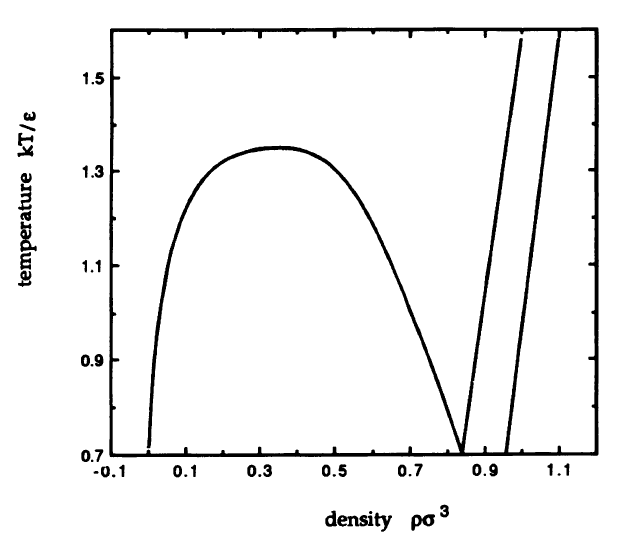
\includegraphics[width=0.4\textwidth]{pauli_gas/phase_diagram_LJ.png}
	\caption{Diagrama de fases de un gas interactuando mediante Lennard-Jones. 
	Esto nos asegura que las densidades elegidas $\rho_{LJ,o}^* = 2.9$, $\rho_{LJ,1}^* = 1.05$ y $\rho_{LJ,2}^* = 0.4$ corresponden a gas+líquido, líquido+sólido y sólido.}
	\label{fig:ej_diag_fases}
\end{figure}

Usaremos estas simulaciones a modo de control, para poder apreciar mejor la fenomenología introducida por el potencial de Pauli.
Sin más preambulos, a continuación se encuentran los resultados.


\subsection{Distribución de impulsos}

El enfriamiento se realizó reduciendo la temperatura por etapas, esperando a que termalizara en la nueva temperatura y posteriormente muestreando el estado 
$(\mathbf{q}_1, ..., \mathbf{q}_N;\mathbf{p}_1, ..., \mathbf{p}_N)$ del sistema (las $6N$ coordenadas).
Este proceso de enfriamiento+muestreo se realizó 8 veces en total, inicializando distintas semillas, para tener una mayor cantidad de muestras y mayor descorrelación entre ellas.
En total, se tomaron $200\times 8 = 1600$ muestras del sistema para cada temperatura.

Con toda esa información, hicimos los histogramas de energía cinética del Pauli gas y los comparamos con las distribuciones de Maxwell-Boltzmann (MB) y Fermi-Dirac (FD)
a esa misma $T$ y $\rho$ y con la misma masa $m$, según las ecuaciones \eqref{eq:dist_MB} y \eqref{eq:dist_FD}, respectivamente.

Comenzando con los parámetros \eqref{eq:params_dorso}, vemos los histogramas de las 3 densidades en las \textbf{Figuras \ref{fig:hist_rho0_dorso}}, 
\textbf{\ref{fig:hist_rho1_dorso}} y \textbf{\ref{fig:hist_rho2_dorso}} para algunas temperaturas seleccionadas.

\begin{figure}[H]
	\centering
	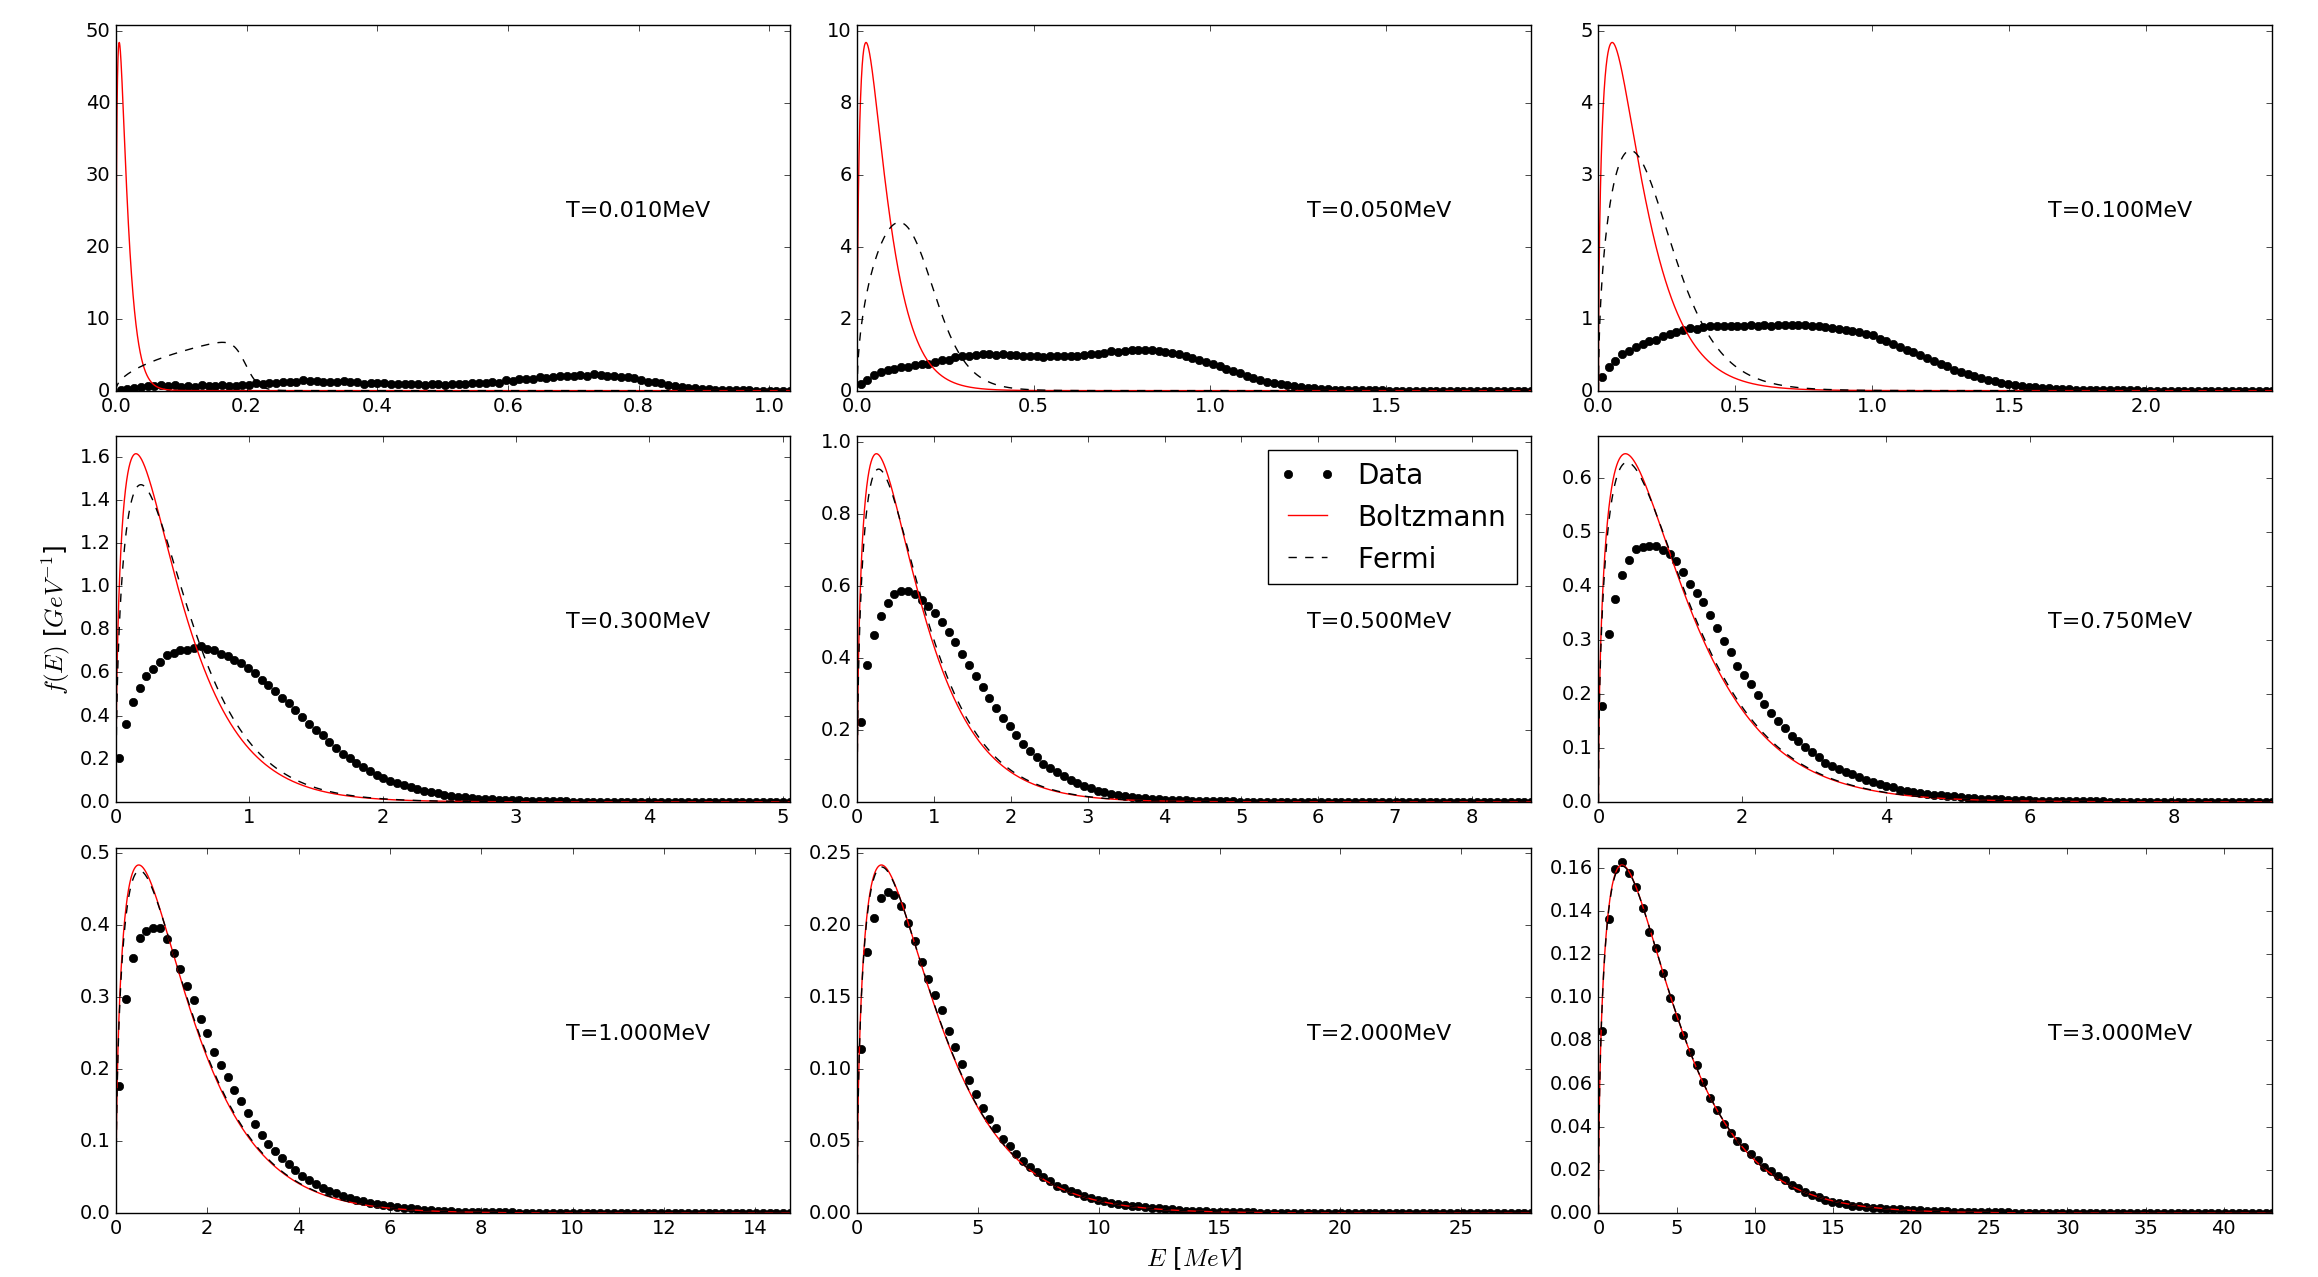
\includegraphics[width=0.9\textwidth]{pauli_gas/hist_rho0_dorso.png}
	\caption{Distribuciones de energía cinética para los parámetros de Dorso en \eqref{eq:params_dorso} y $\rho^* = \rho_o^* = 3.375$}
	\label{fig:hist_rho0_dorso}
\end{figure}

\begin{figure}[H]
	\centering
	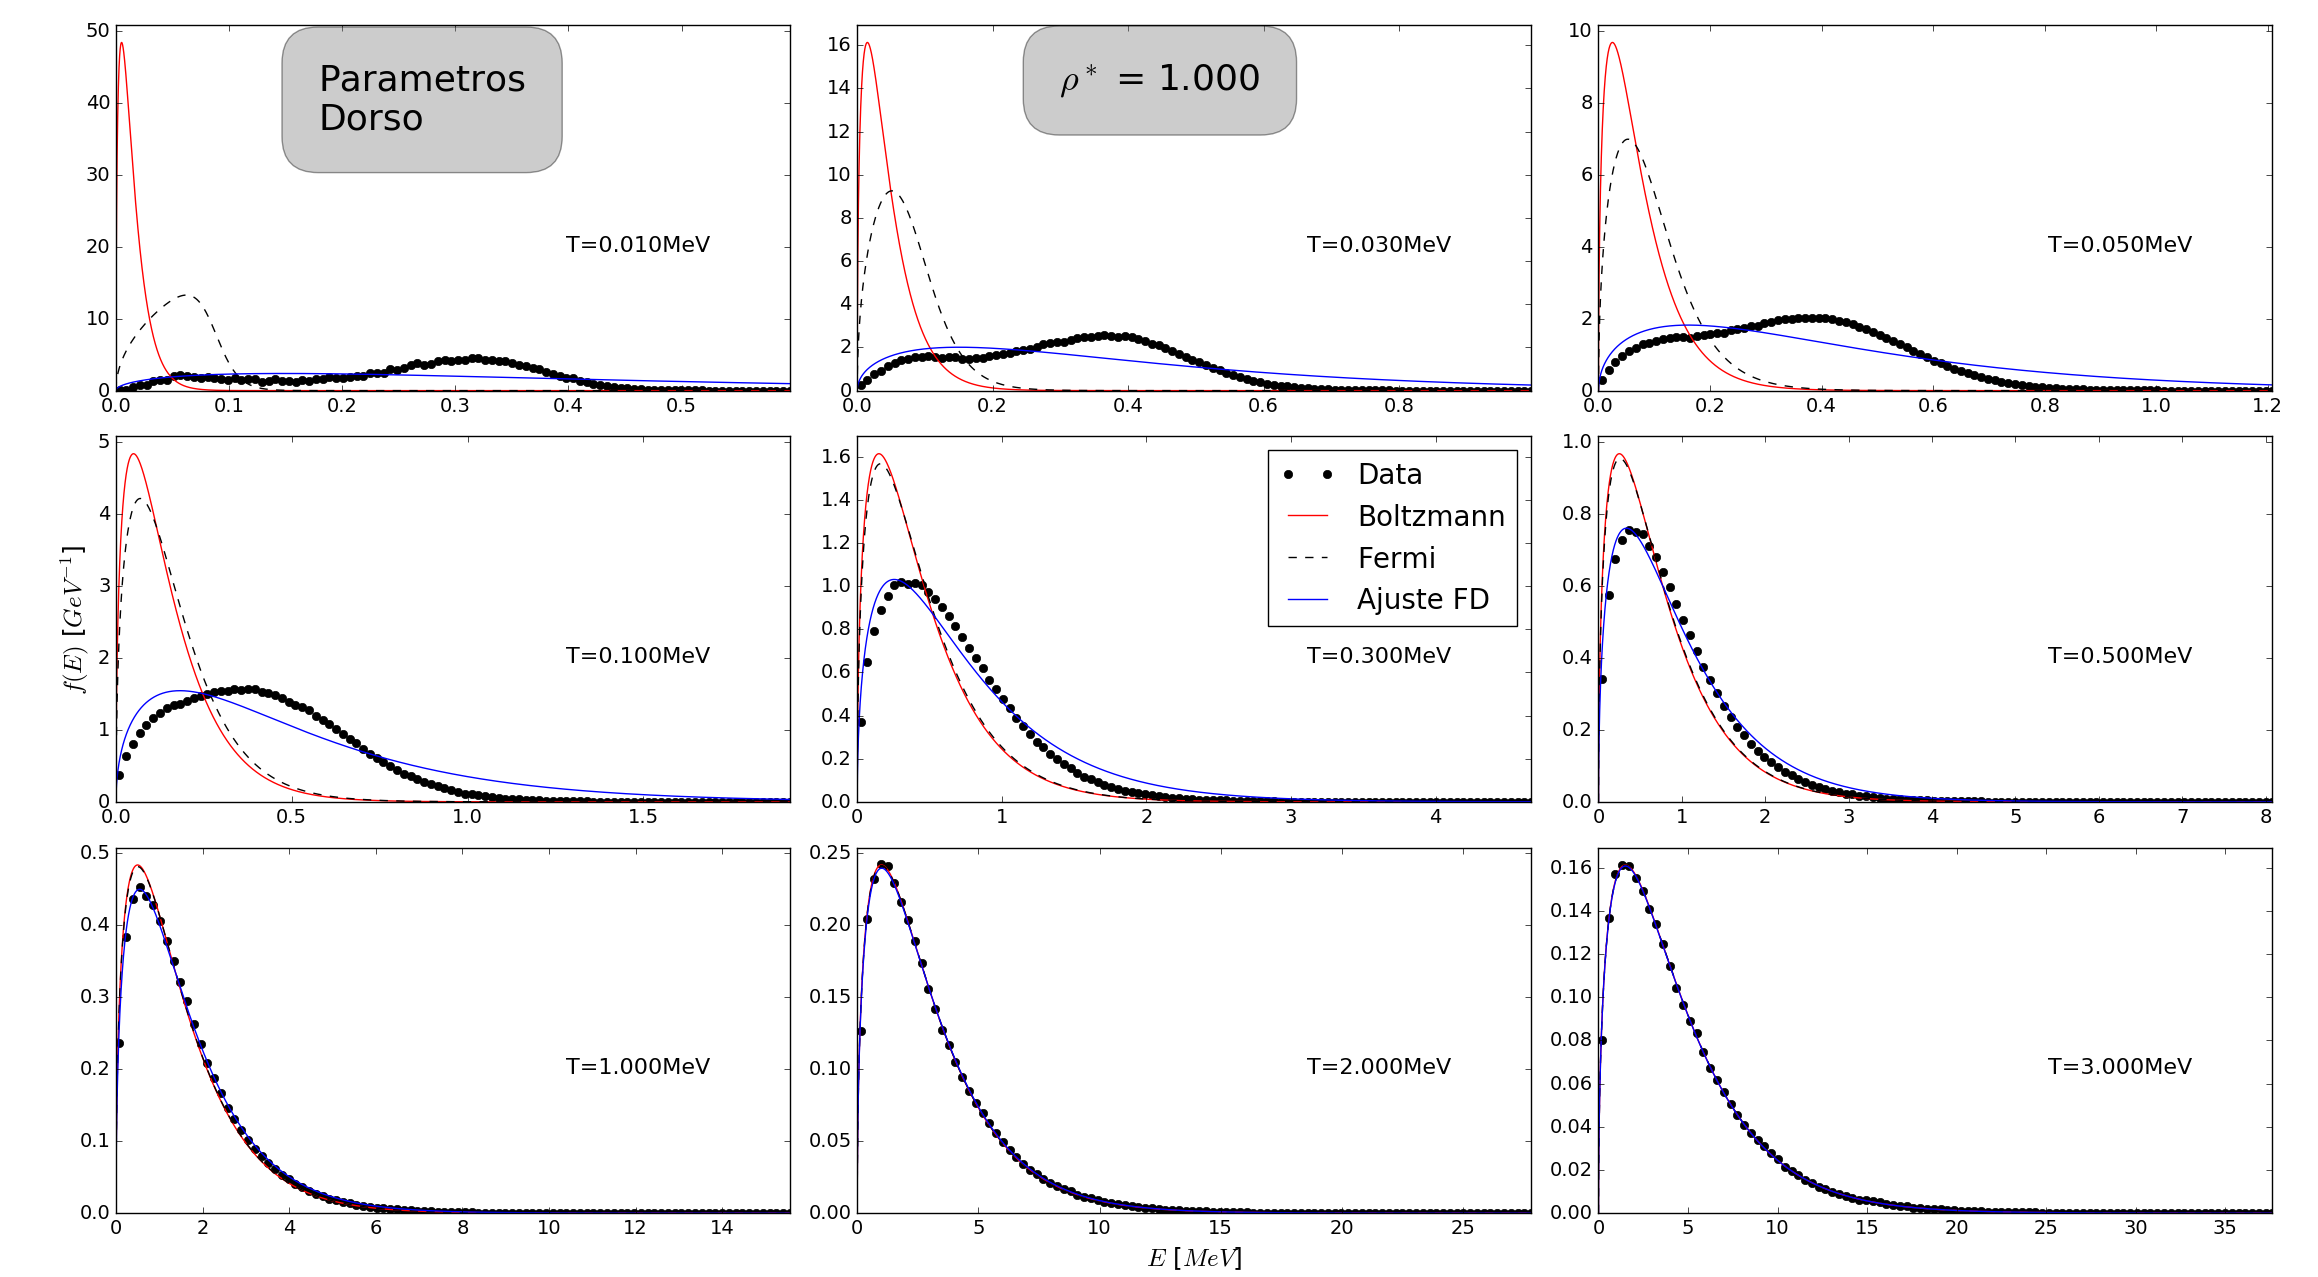
\includegraphics[width=0.9\textwidth]{pauli_gas/hist_rho1_dorso.png}
	\caption{Distribuciones de energía cinética para los parámetros de Dorso en \eqref{eq:params_dorso} y $\rho^* = \rho_1^* = 1$}
	\label{fig:hist_rho1_dorso}
\end{figure}
\begin{figure}[H]
	\centering
	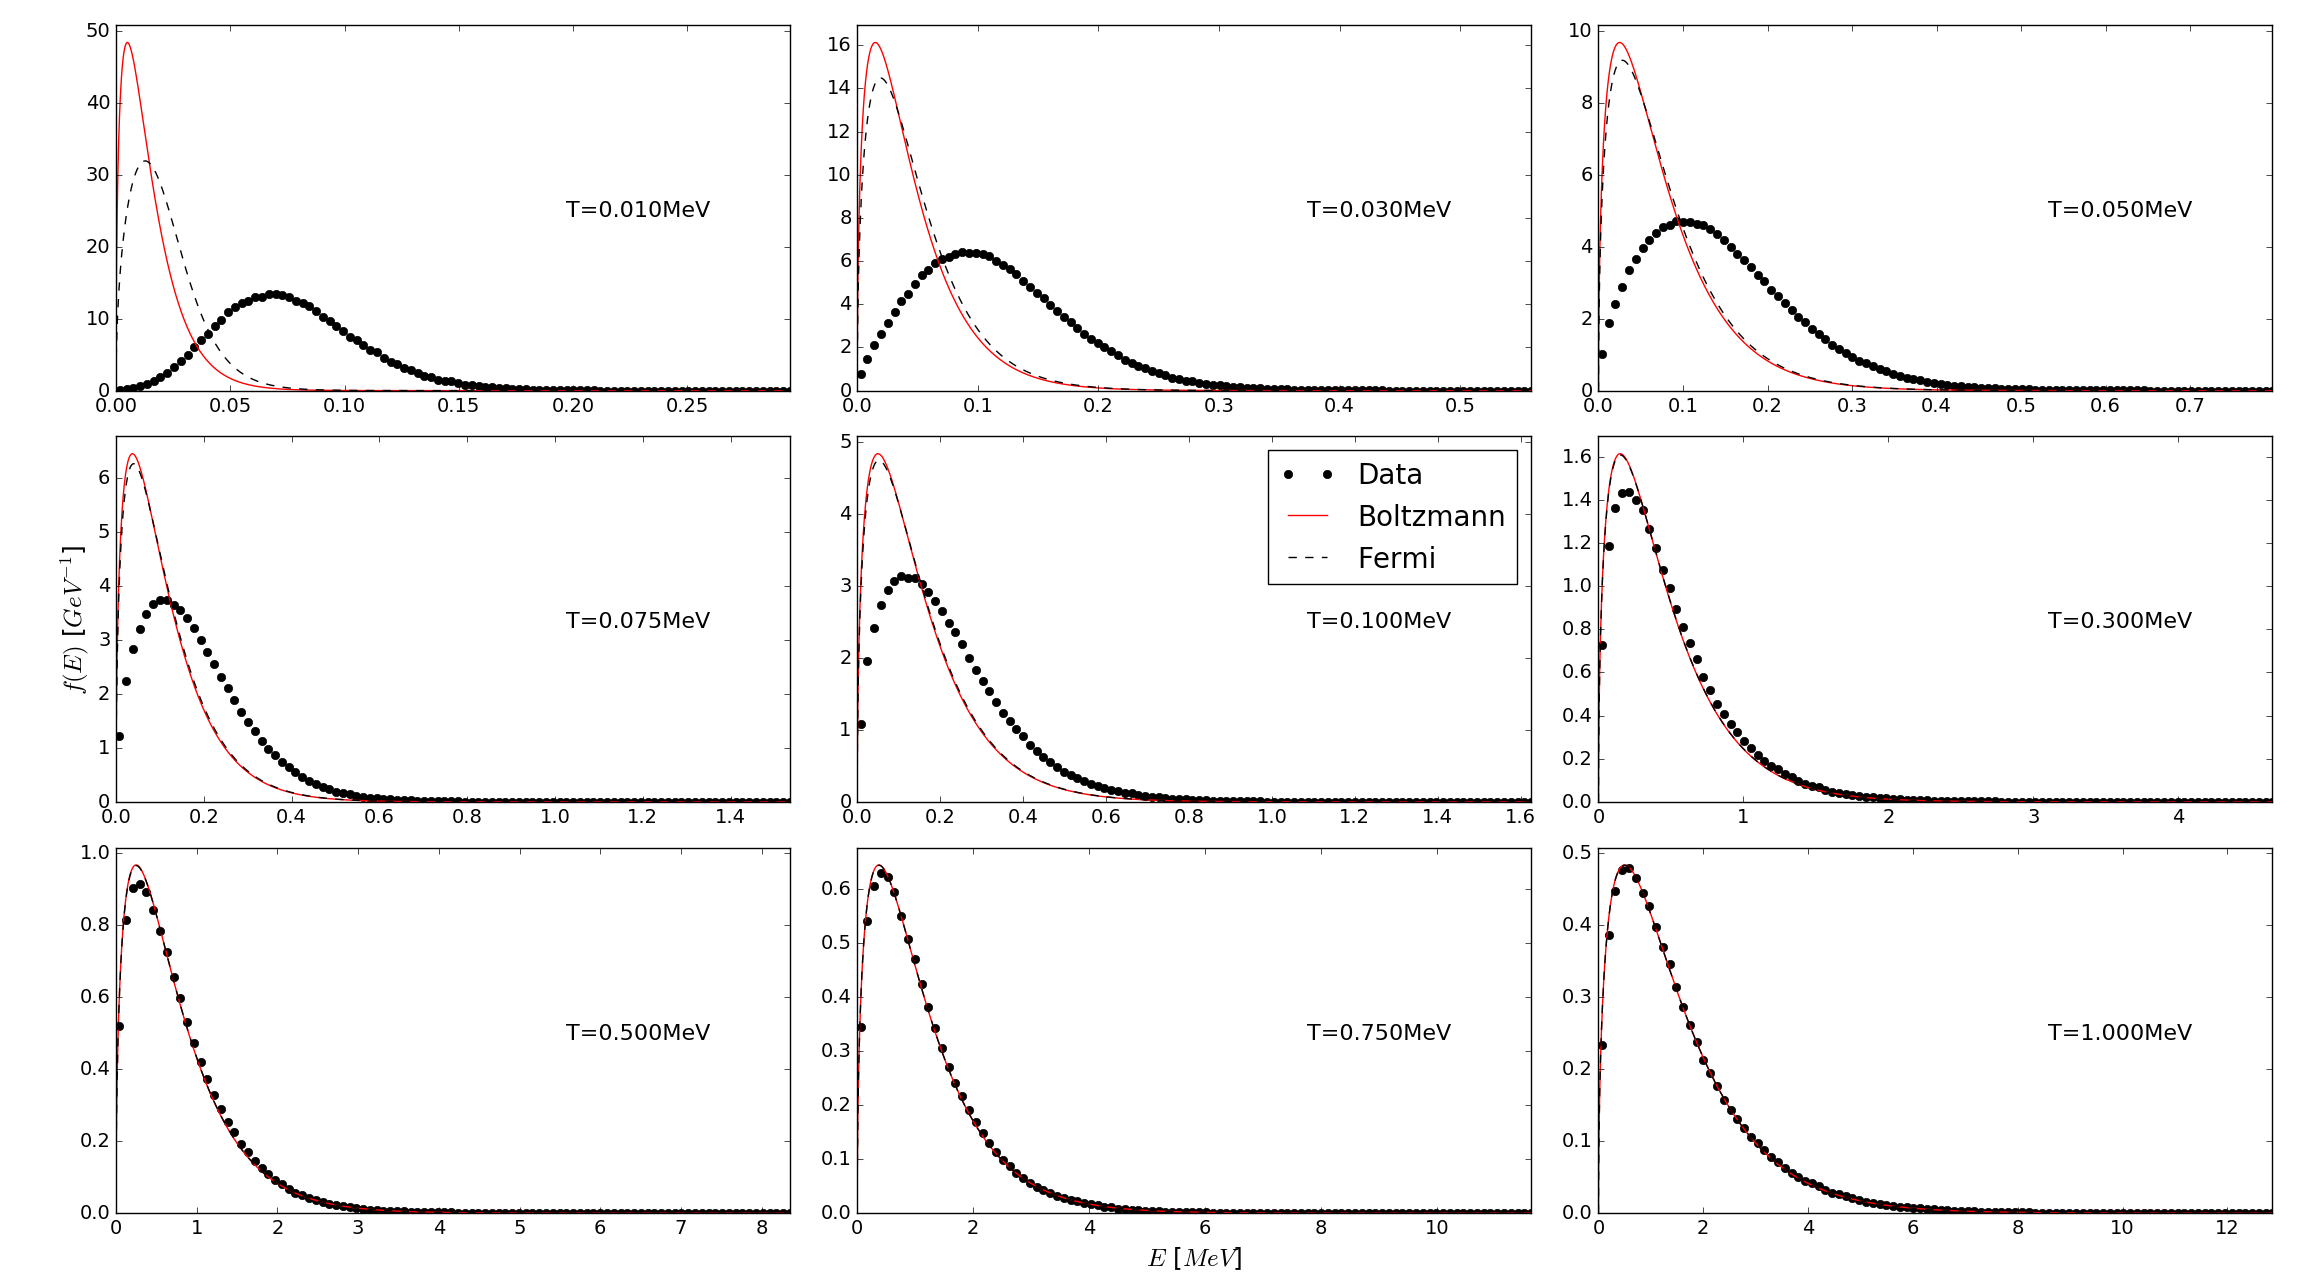
\includegraphics[width=0.9\textwidth]{pauli_gas/hist_rho2_dorso.png}
	\caption{Distribuciones de energía cinética para los parámetros de Dorso en \eqref{eq:params_dorso} y $\rho^* = \rho_2^* = 0.125$}
	\label{fig:hist_rho2_dorso}
\end{figure}

En los 3 casos, podemos apreciar como la distribución se aleja de MB a medida que la temperatura desciende según lo esperado.
Sin embargo, esta separación comienza a una temperatura mayor que la separación de FD respecto a MB.
De hecho, los datos no tienden a acercarse a FD luego de alejarse de MB; solo hay coindicencia de las 3 distribuciones (simultaneamente) a $T$ alta.
Similar a FD, el pico del histograma de los datos no parece acercarse al origen, una de las principales diferencias con MB.
Sin embargo, este pico se da para energías cinéticas mucho mayores que el de FD, lo cual hace pensar que este gas de Pauli sobreestima la exclusión entre las particulas, alejándolas
más de lo que debería.

Más particularmente, podemos notar que la distribución a $T$ baja para $\rho_o^*$ y $\rho_1^*$ tiene 2 picos en lugar de uno, lo cual es muy llamativo.
Para $\rho_2^*$, solo hay un máximo, pero la curva entre este máximo y el origen es cóncava en lugar de convexa a diferencia tanto de MB como FD como de las otras densidades.
Además, la separación de los datos respecto a MB se da a temperaturas cada vez menores a medida que aumentamos $\rho^*$, lo cual también ocurre con FD.
Esto es razonable, dado que la noción de temperatura alta está muy asociada a la de densidad baja como discutimos en \ref{sec:intro_fermi_gas}.

Con los histogramas obtenidos utilizando los parámetros de Maruyama \eqref{eq:params_maruyama} ocurre algo muy similar, como puede verse en las \textbf{Figuras \ref{fig:hist_rho0_maruyama}}, 
\textbf{\ref{fig:hist_rho1_maruyama}} y \textbf{\ref{fig:hist_rho2_maruyama}}.
Sin embargo, es ciertamente notable que la forma del histograma de los datos parece acompañar mejor a la distribución de FD.
Además, surge inmediatamente la diferencia de escalas entre temperaturas; las transiciones de las distribuciones del Pauli gas ocurren a $T$ un orden de magnitud mayor para estos parámetros.
Esto es llamativo y puede ciertamente estar asociado al hecho de que el $D^*$ mismo aumentó un orden de magnitud.

Esto ocurre en menor medida para la distribución de FD.
Es razonable que ocurra dado que, aunque los $\rho^*$ no cambiaron, si lo hicieron las densidades $\rho$ al cambiar el $q_o$.
Dado que el $q_o$ de Maruyama es menor, las densidades $\rho$ aumentaron, redefiniendo la noción de alta temperatura para valores de $T$ mayores.

Esto ciertamente nos muestra que el parámetro $q_o$ también influye a la hora de simular una distribución de FD vía un gas de Pauli.

Para entender esto, podemos nuevamente adimensionalizar el problema, analizando los parámetros que definen la forma de las distintas distribuciones.
Dado que las distribuciones de energía cinética $f(\varepsilon)$ son extensivas, podemos obtener una magnitud intensiva del sistema dividiendolas por el número de partículas $N$.
Esta nueva distribución intensiva solo puede depender de parámetros intensivos del sistema, como son la temperatura $T$ y la densidad $\rho$ pero también de parámetros microscópicos como
la masa $m$ y la constante de Planck $\hbar$.
Recordando las expresiones de $f_{FD}(\varepsilon)$ y $f_{MB}(\varepsilon)$ de \eqref{eq:dist_FD} y \eqref{eq:dist_MB}, vemos inmediatamente que podemos reescribir
\[ f_{MB}(\varepsilon;N,T) = \frac{N}{T}g_{MB}(\varepsilon^*) \]
\[ f_{FD}(\varepsilon;N, V, T, m, \hbar) = \frac{N}{T}g_{FD}(\varepsilon^*;\lambda^3\rho) \]
donde $\varepsilon^* = \varepsilon/T$ y $\lambda$ es la longitud de onda términa previamente definida.
En resumen, la adimensionalización nos permite eliminar 3 variables, mientras que la linealidad en $N$ nos permite eliminar una cuarta.

Podemos hacer un razonamiento análogo para la distribución $f_P(\varepsilon)$ de un gas de Pauli.
Los parámetros relevantes siguen siendo $T$, $\rho$ y $m$ pero también se suman los $D$, $q_o$ y $p_o$ del potencial de Pauli.
Una adimensionalización como la de \ref{sec:adim_choque1d} arrojaría inmediatamente 
\[ f_P(\varepsilon; N,V,T, m D, q_o,p_o.) = \frac{N}{T}g_P(\varepsilon^*; D^*, T^*, \rho^*)\]
con la definición habitual $D^*=Dm/p_o^2$, $T^*=Tm/p_o^2$ y $\rho^* = \rho q_o^3$.

Bajo estas consideraciones, la única diferencia entre la $f_P$ obtenida con los distintos parámetros para Pauli se debe $D^*$ y $T^*$ (pues mantuvimos $\rho^*$); a los parámetros $D$ y $p_o$.
Sin embargo, la similitud entre $f_P$ y $f_{FD}$ cambia pues $f_{FD}$ depende de $\rho$ en lugar de $\rho^*$, reescalando las temperaturas.
Esto en principio parecería indicar que todos los parámetros del potencial de Pauli son relevantes a la hora de emular la distribución de FD.

\begin{figure}[H]
	\centering
	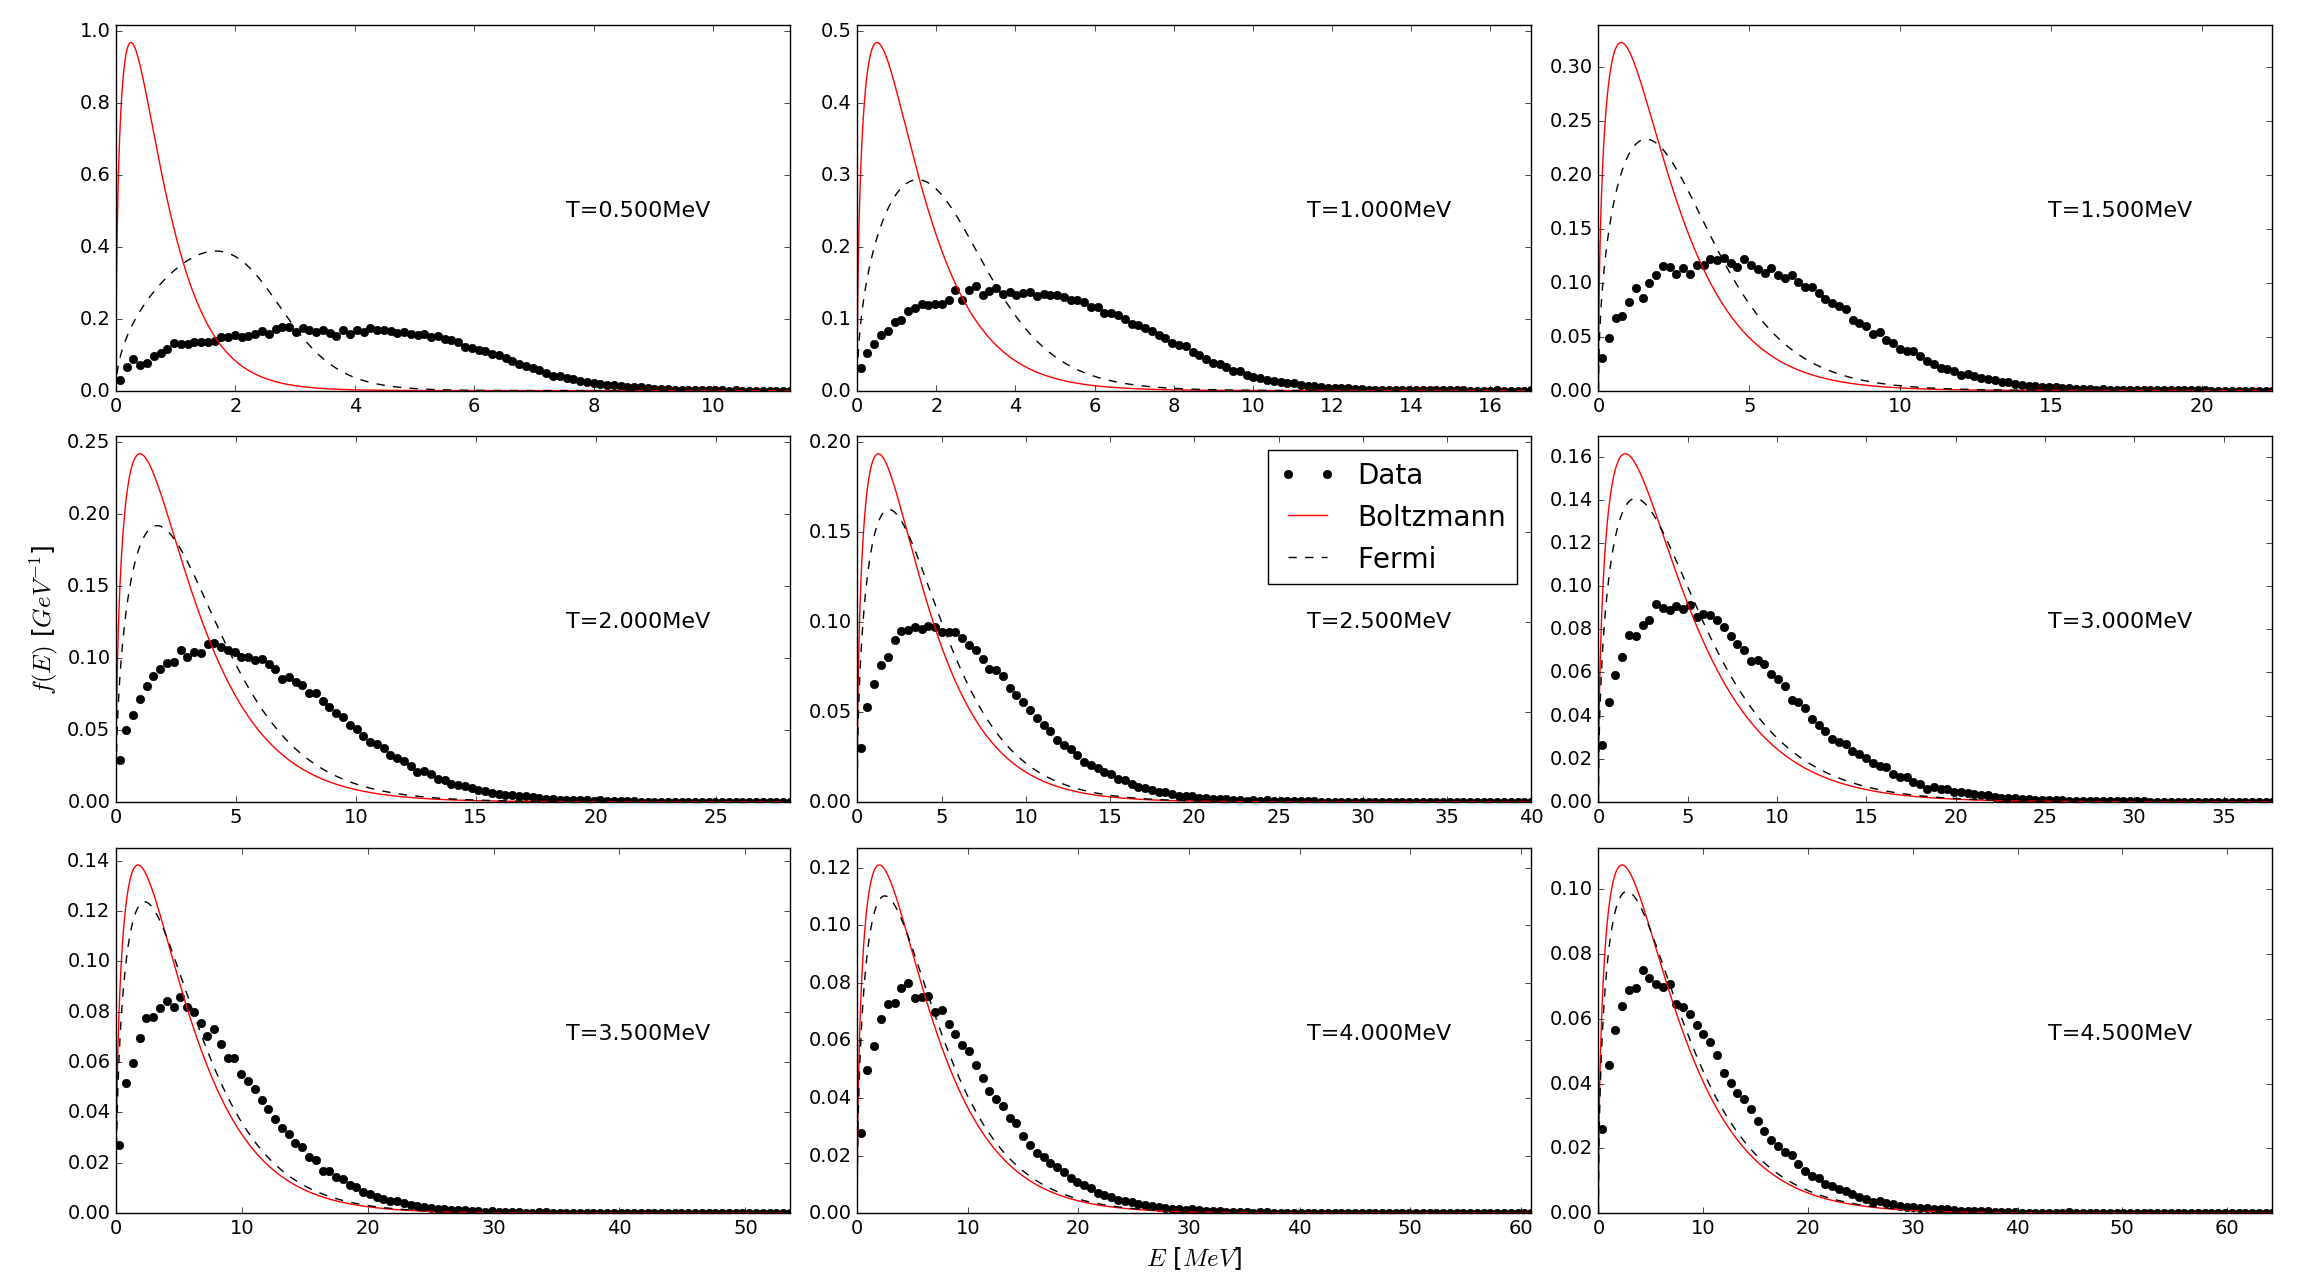
\includegraphics[width=0.9\textwidth]{pauli_gas/hist_rho0_maruyama.png}
	\caption{Distribuciones de energía cinética para los parámetros de Maruyama en \eqref{eq:params_maruyama} y $\rho^* = \rho_o^* = 3.375$}
	\label{fig:hist_rho0_maruyama}
\end{figure}

\begin{figure}[H]
	\centering
	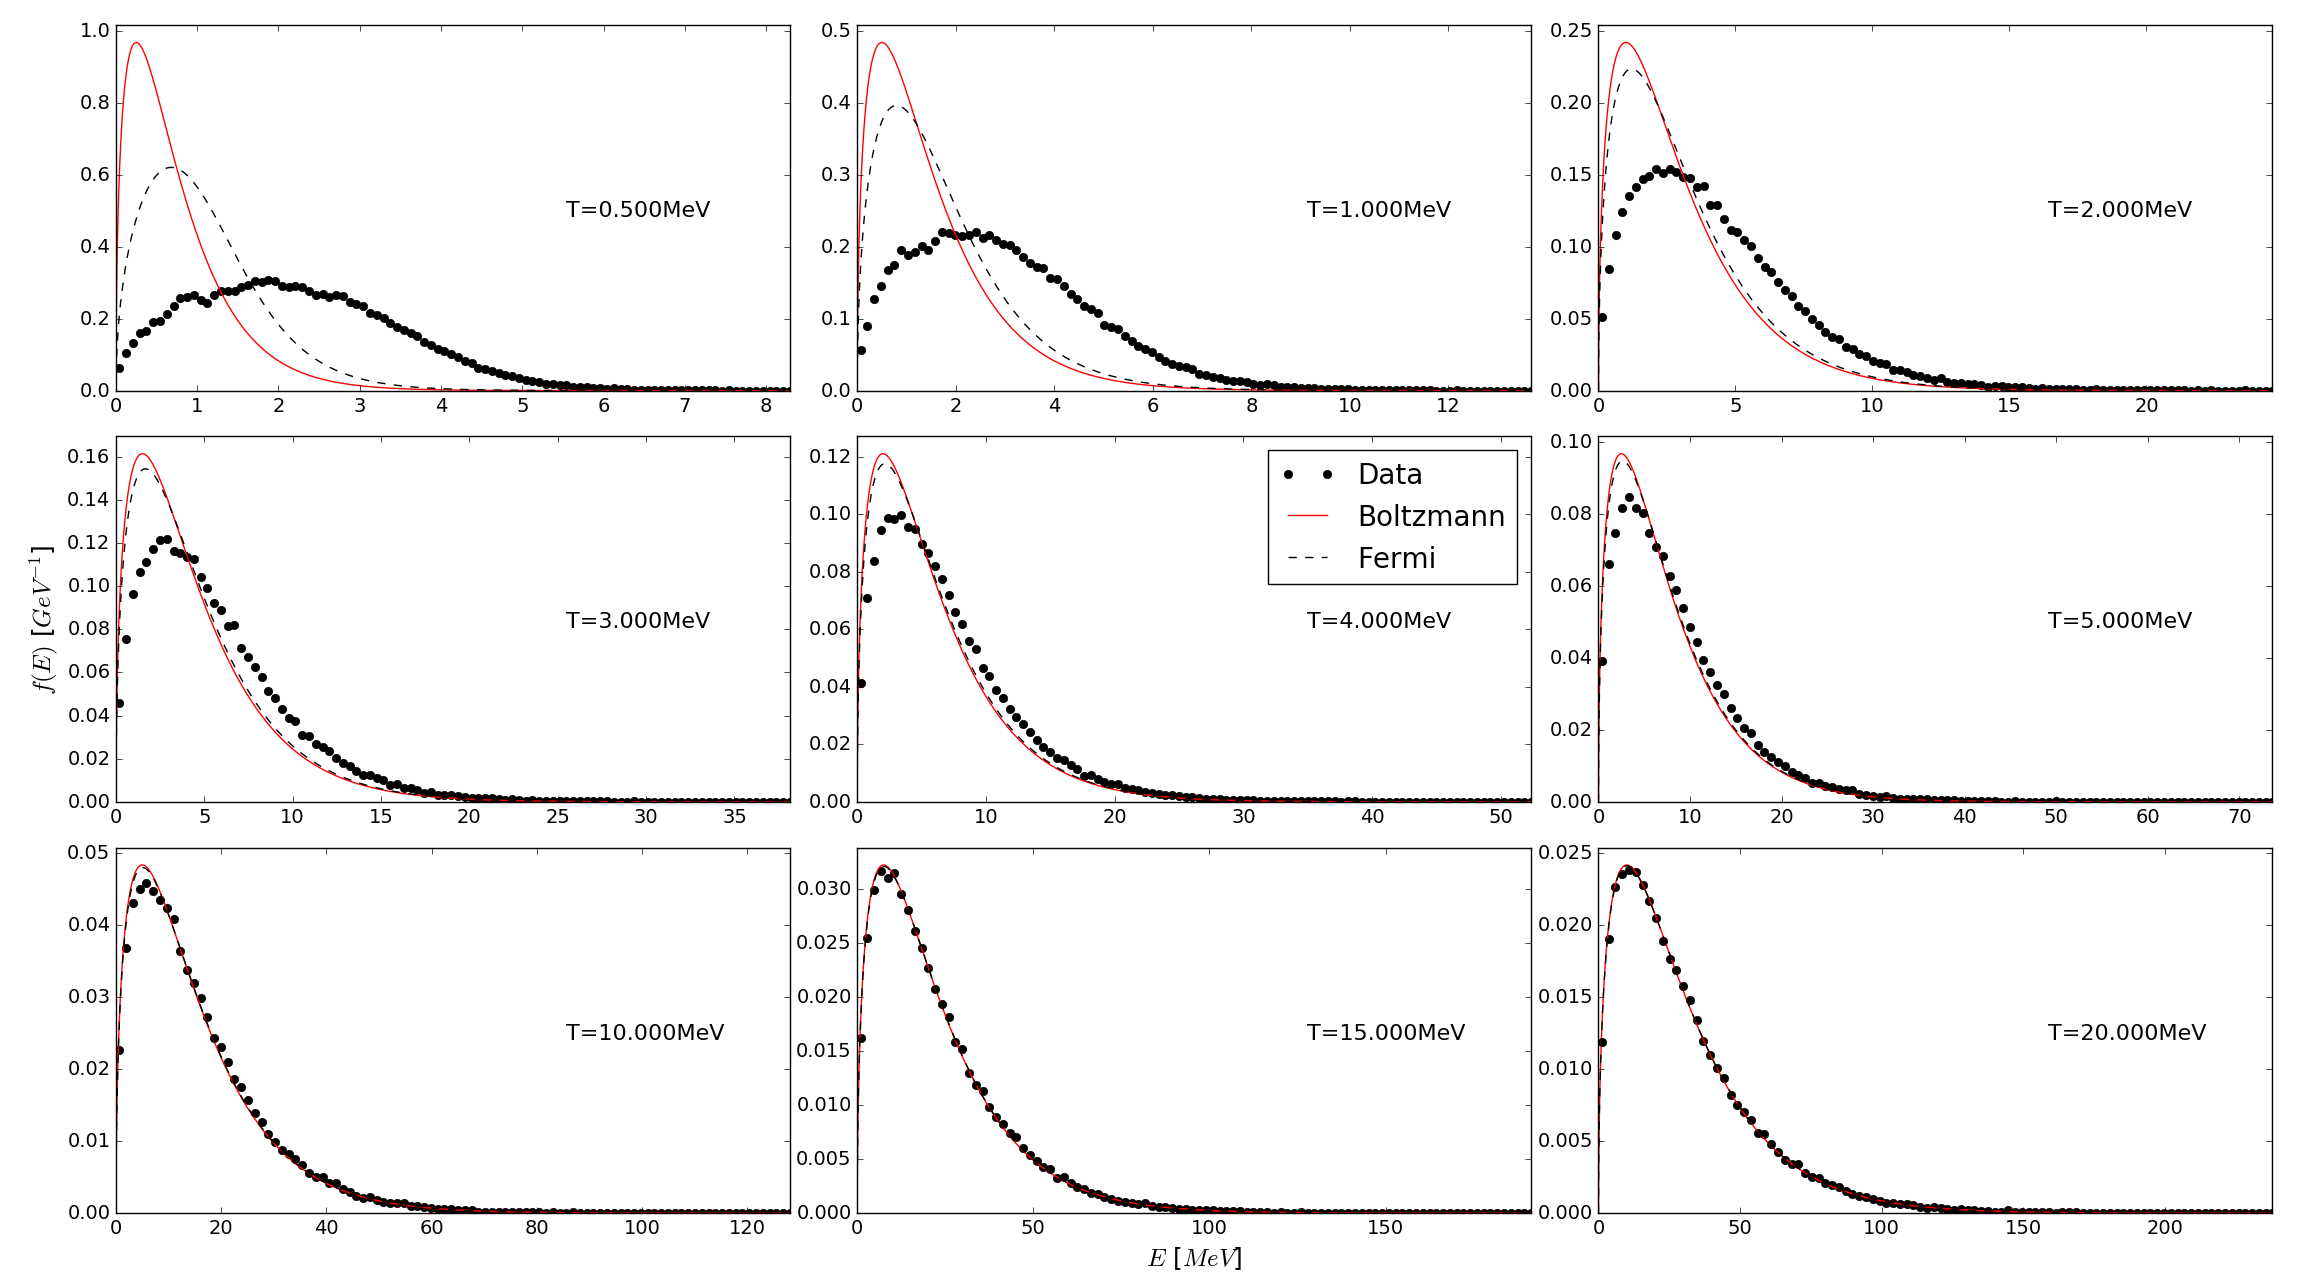
\includegraphics[width=0.9\textwidth]{pauli_gas/hist_rho1_maruyama.png}
	\caption{Distribuciones de energía cinética para los parámetros de Maruyama en \eqref{eq:params_maruyama} y $\rho^* = \rho_1^* = 1$}
	\label{fig:hist_rho1_maruyama}
\end{figure}
\begin{figure}[H]
	\centering
	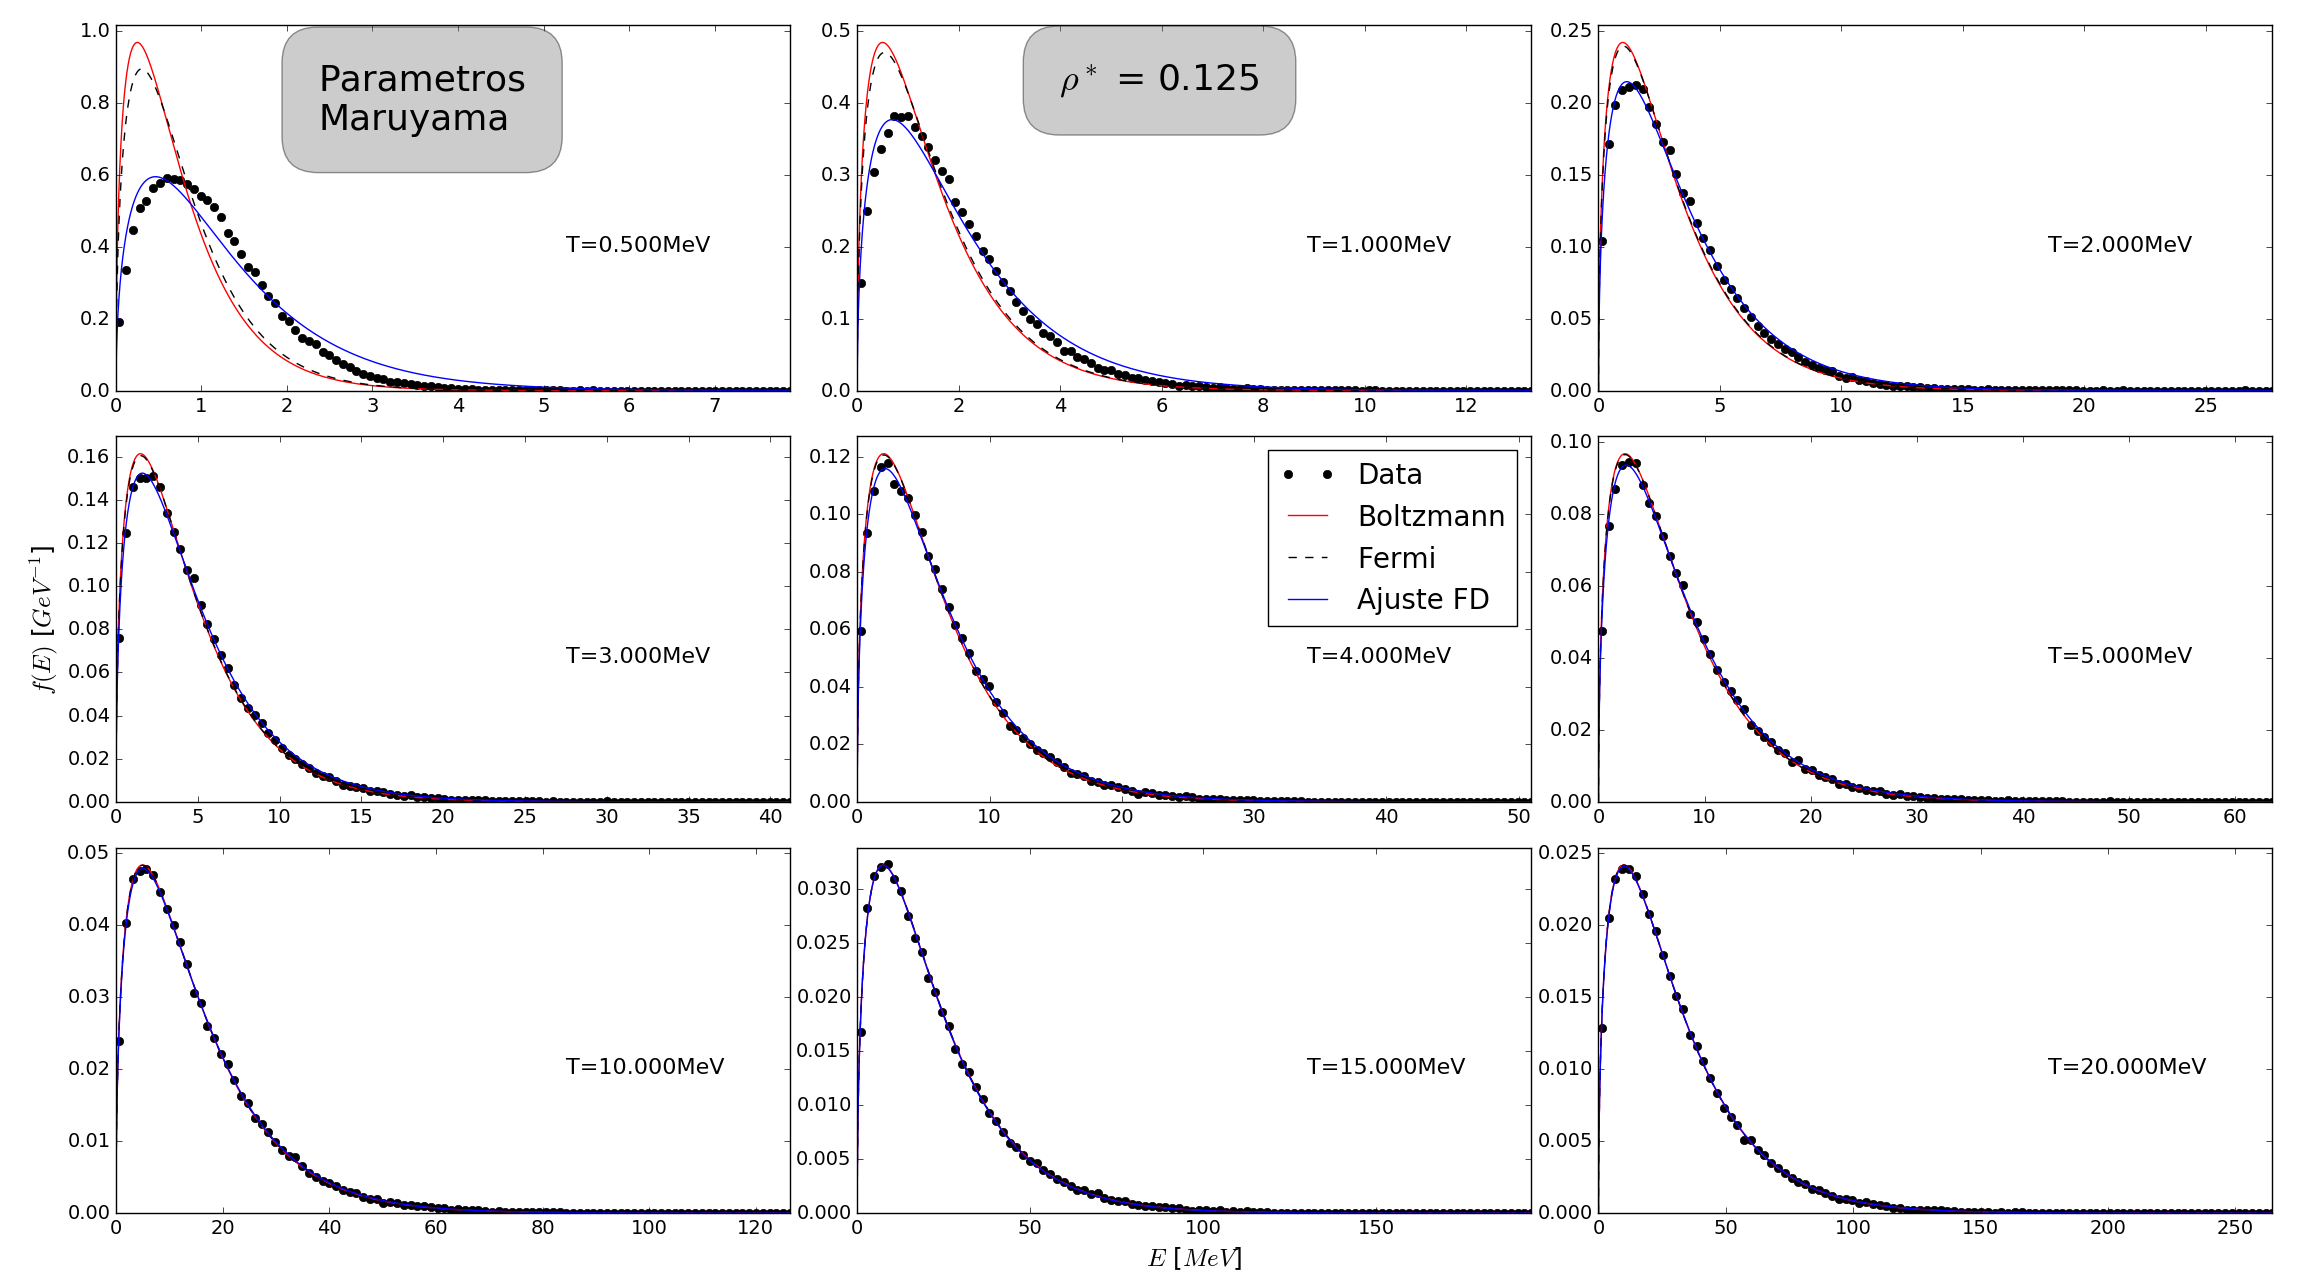
\includegraphics[width=0.9\textwidth]{pauli_gas/hist_rho2_maruyama.png}
	\caption{Distribuciones de energía cinética para los parámetros de Maruyama en \eqref{eq:params_maruyama} y $\rho^* = \rho_2^* = 0.125$}
	\label{fig:hist_rho2_maruyama}
\end{figure}

Esto último resulta razonable si consideramos que la forma de la región excluída también es relevante para el problema.
Su forma resulta basicamente elíptica, pero los parámetros $q_o$ y $p_o$ regulan sus ejes.
Sin embargo, a priori no es posible afirmar que estos parámetros $D$, $q_o$ y $p_o$ puedan ser independientes de la temperatura $T$ y $\rho$.
Esto ciertamente es deseable, pero un estudio pormenorizado de estas cuestiones excede el alcance de este trabajo.

Por último, mostramos en las \textbf{Figuras \ref{ }}, \textbf{\ref{ }} y \textbf{\ref{ }} las distribuciones de energía cinética obtenidas para un gas de LJ.
En contraposición a lo anterior, su distribución resulta idénticamente la de MB.


\subsection{Area excluída}



\subsection{Presión}

\section{Nuclear Matter}{\label{sec:NM}}
%\subsection{Primeras simulaciones}

El objetivo de esta sección es analizar la influencia del potencial de Pauli \eqref{eq:def_int_pauli} en la simulación de NM. 
Como dijimos, el potencial nuclear de QCNM \eqref{eq:pot_QCNM} no distingue entre protones y neutrones, por lo que a efectos de ese potencial tenemos $N=N_n+N_p$ partículas idénticas.
Con la introducción del potencial de Pauli, separaremos las $N=1000$ partículas según sus componentes de spin e isospin, por lo que $N = N_n^\uparrow+N_n^\downarrow+N_p^\uparrow+N_p^\downarrow$.
En particular, nos interesa un caso simétrico, tomamos $N_n^\uparrow=N_n^\downarrow=N_p^\uparrow=N_p^\downarrow = N/4 = 250\equiv n$.
Dado que la exclusión de Pauli solo puede darse para partículas con la misma componente de spin e isospin, tendremos $N(N-1)/2$ pares de interacción nuclear y $4n(n-1)/2 = N(N/4-1)/2$ pares de 
interacción de Pauli. 
Utilizaremos los parámetros de Dorso \eqref{eq:params_dorso} en el potencial de Pauli.

Las densidades habituales de NM resultan del orden de $0.1$fm$^{-3}$, que para un sistema de $N=1000$ partículas exige cajas de lado $L\sim 20$fm.
Si recordamos que previamente impusimos un $s_{cut}^2=10$ para el potencial se Pauli, equivalente a una distancia de $s_{cut}q_o \approx 19$fm, vemos inmediatamente que utilizar un criterio de
mínima imagen resulta inviable al exigir $r_{cut}\leq L/2$, necesitariamos aumentar la cantidad de partículas a $N\sim8000$ para alcanzar densidades $\rho=0.3$fm$^{-3}$.

Es por esto que decidimos usar las condiciones periódicas del sistema sin el criterio de mínima imagen, permitiendo la interacción simultánea con múltiples imagenes de una misma partícula.
Agregando $l$ copias del sistema en cada una de las direcciones (llamadas \textit{layers}), nos basta que $r_{cut}\leq l.L$ para asegurar que no estamos perdiendo interacciones.
Con el objetivo de tener la menor cantidad de \textit{layers} posibles para reducir el costo computacional, reducimos la distancia de corte de Pauli a $s_{cut}=6$fm, donde el potencial cae a un $5\%$
del valor máximo $D$.
Dado que el potencial nuclear tiene un $r_{cut}^{(N)} = 6$fm$\leq r_{cut}^{(P)} = 14.7$fm, nos basta elegir un $l$ que cumpla $l.L \geq 14.7$fm.
Sin embargo, el valor de $L$ dependerá de $\rho$, por lo que si acotamos $\rho\leq 0.3$fm$^{-3}$ vemos que nos basta tomar $l=1$.
Por lo tanto, una única capa de imagenes bastará para nuestras simulaciones.

Dado que nos interesa el estado fundamental de NM, haremos simulaciones de montecarlo para $T=0.5$MeV, comenzando el sistema como una red simple cúbica con impulsos según la distribución de Boltzmann
a esa $T$.
Esto lo hicimos para múltiples densidades $\rho$ entre $0.005$fm$^{-3}$ y $0.3$fm$^{-3}$
Evolucionamos el sistema hasta que la energía se estabilizara, para lo cual bastaron $10^5N$ pasos para todas las densidades $\rho$ estudiadas.

\newpage
\begin{figure}[H]
	\centering
	\subfigure[$\rho=0.005$fm$^{-3}$]{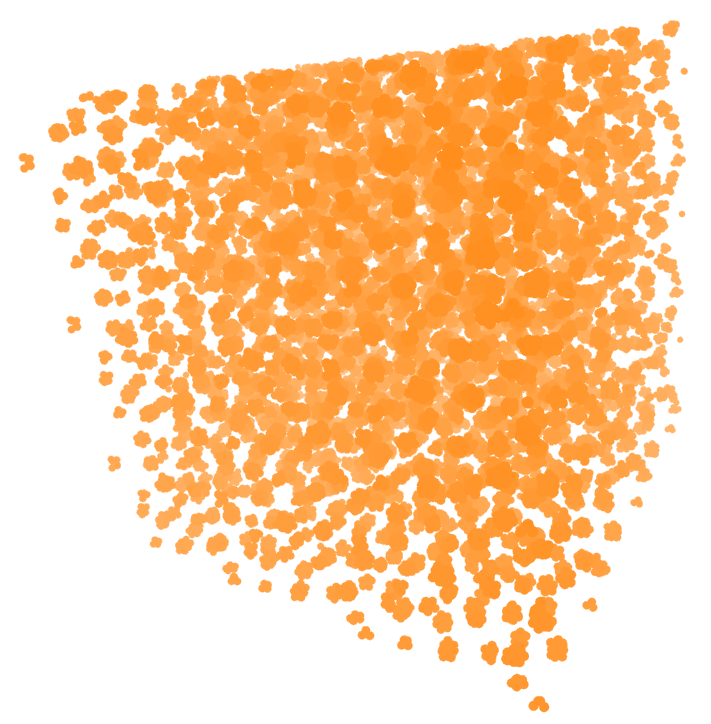
\includegraphics[width=0.3\columnwidth]{NM/pastas_x1/noquis_0,005_x1.png}}
	\hspace{0.03\columnwidth}
	\subfigure[$\rho=0.03$fm$^{-3}$]{
\includegraphics[width=0.3\columnwidth]{NM/pastas_x1/noquis_0,03_x1.png}}
	\hspace{0.03\columnwidth}
	\subfigure[$\rho=0.04$fm$^{-3}$]{
\includegraphics[width=0.3\columnwidth]{NM/pastas_x1/noquis-fideos_0,04_x1.png}}
	\subfigure[$\rho=0.05$fm$^{-3}$]{
\includegraphics[width=0.3\columnwidth]{NM/pastas_x1/fideos_0,05_x1.png}}
	\hspace{0.03\columnwidth}
	\subfigure[$\rho=0.06$fm$^{-3}$]{
\includegraphics[width=0.3\columnwidth]{NM/pastas_x1/fideos-lasagna_0,06_x1.png}}
	\hspace{0.03\columnwidth}
	\subfigure[$\rho=0.08$fm$^{-3}$]{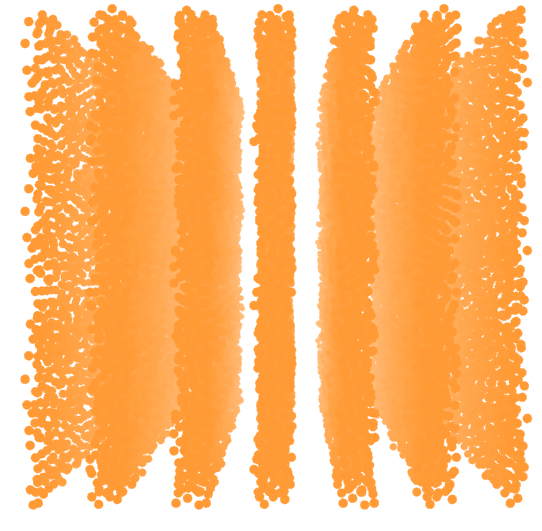
\includegraphics[width=0.3\columnwidth]{NM/pastas_x1/lasagna_0,08_x1.png}}
	\subfigure[$\rho=0.125$fm$^{-3}$]{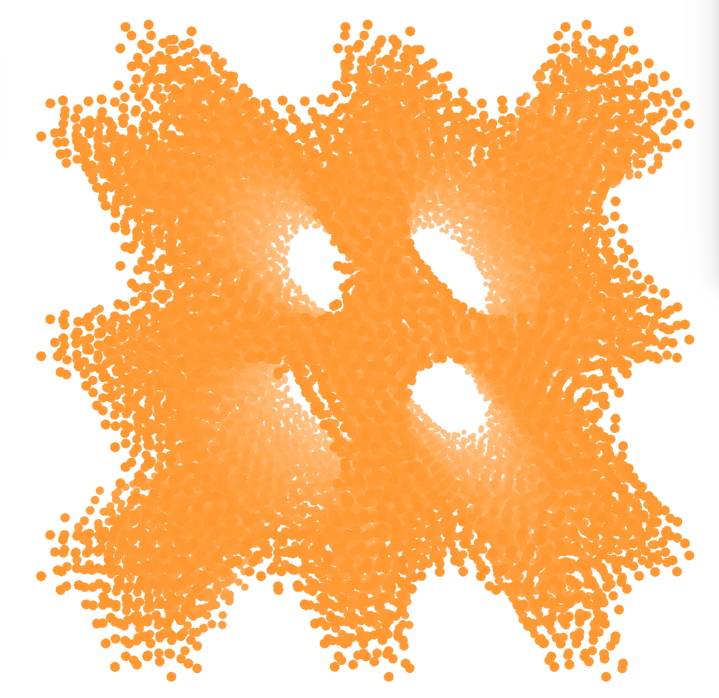
\includegraphics[width=0.3\columnwidth]{NM/pastas_x1/tuneles_0,125_x1.png}}
	\hspace{0.03\columnwidth}
	\subfigure[$\rho=0.16$fm$^{-3}$]{
\includegraphics[width=0.3\columnwidth]{NM/pastas_x1/burbuja_0,16_x1.png}}
	\hspace{0.03\columnwidth}
	\subfigure[$\rho=0.175$fm$^{-3}$]{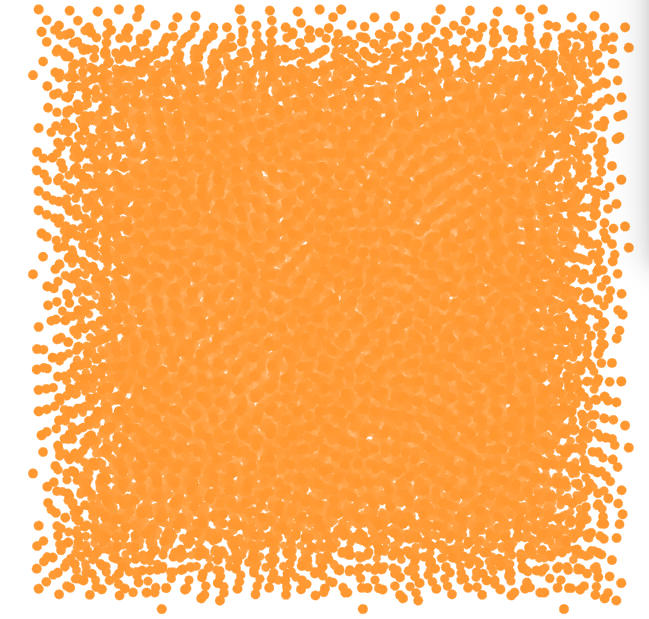
\includegraphics[width=0.3\columnwidth]{NM/pastas_x1/gas_0,175_x1.png}}
	\caption{Distintas topologías halladas durante la simulación.
	También se muestra una layer adicional de imagenes para facilitar visualización.}
	\label{fig:pastas_x1}
\end{figure}

Los resultados de estas simulaciones fueron inesperados.
Para empezar, en la \textbf{Figura \ref{fig:pastas_x1}} podemos ver las configuraciones de algunas densidades seleccionadas.
Estas configuraciones se muestran con la primer capa de imagenes para poder apreciar mejor las pastas resultantes.
En los casos de fideos y lasagnas, podemos ver que tenemos más de una estructura por celda, algo no habitual en NM.
Además, se muestran configuraciones menos definidas en $\rho=0.04$fm$^{-3}$ y $\rho=0.06$fm$^{-3}$, probablemente densidades muy cercanas a la transición entre pastas.
Para $\rho\geq 0.17$fm$^{-3}$ las pastas desaparecen y dan lugar a un gas uniforme. 

Lo más extraño, sin embargo, es la tendencia de los ñoquis a reducir su tamaño a medida que $\rho$ baja. 
Para $\rho=0.03$fm$^{-3}$ el sistema está compuesto de ñoquis de $\sim 100$ partículas, pero al alcanzar $\rho=0.005$fm$^{-3}$ el tamaño descendió a $\sim 10$ partículas.
Esto parecería indicar que en el límite de bajas densidades $\rho\to0$ el estado fundamental del sistema resulta el de partículas individuales no interactuantes, lo cual no es consistente con 
la existencia de núcleos atómicos. 
En particular, implica que la repulsión dada por el potencial de Pauli supera la atracción del potencial nuclear.
Esta ineficiencia energética de acercar nucleones puede darse por 2 razones; bien Pauli tiene una gran intensidad $D$ o un gran alcance $q_o$. 
El primer caso es obvio, pero el segundo implica que si 2 partículas logran estar muy cerca sus impulsos deben diferir considerablemente, lo cual impone un aumento de la energía cinética.

Más allá de la topología, analizamos la energía por partícula del sistema $E$ en función de $\rho$, esperando encontrar un mínimo en $\rho=0.04$fm$^{-3}$ de $\sim -16$MeV.
En la \textbf{Figura \ref{fig:Evsrho_QCNMx1}} podemos ver que esto no es así, dado que hayamos un mínimo de $\sim -47$MeV en $\rho=0.2$fm$^{-3}$.
Esta energía de ligadura resulta el triple de la esperada, una grosera sobreestimación. 
También se encuentran marcados los distintos regimenes de pasta del sistema. 

\begin{figure}[H]
	\centering
	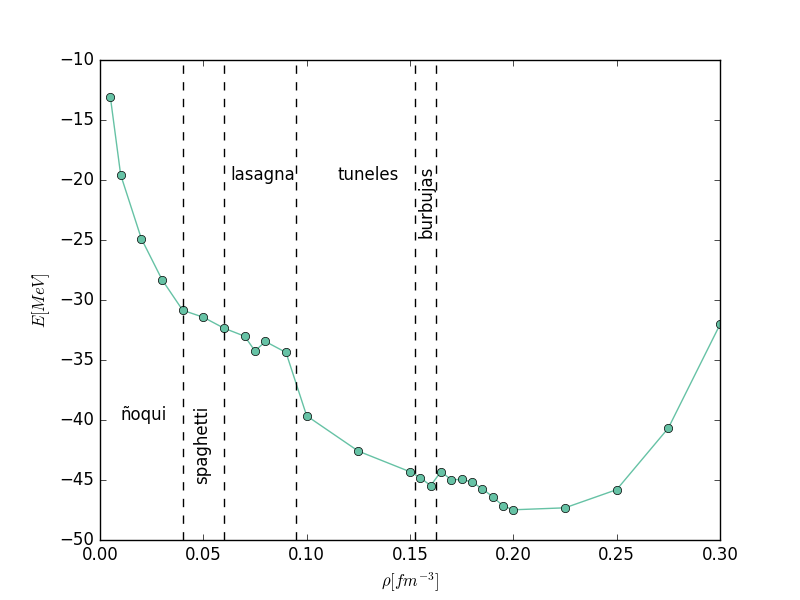
\includegraphics[width=0.9\textwidth]{NM/Evsrho_full_x1.png}
	\caption{}
	\label{fig:Evsrho_QCNMx1}
\end{figure}

\subsection{Reajuste de parámetros y enfriamiento}

Viendo la sobreestimación de las energías de ligadura de la \textbf{Figura \ref{fig:Evsrho_QCNMx1}}, la respuesta natural fue buscar reducir esta energía.
Para esto, resultó natural reducir la intensidad $V_o$ del potencial nuclear presentado en \ref{sec:intro_NM} a la mitad.
Con el objetivo adicional de estudiar la formación de estas pastas, inicializamos el sistema en $T=5$MeV y lo enfriamos escalonadamente hasta alcanzar los $T=0.5$MeV.
En cada temperatura, muestreamos la energía por partícula para obtener la curva calórica.
En la \textbf{Figura \ref{fig:EvsT_pastas}} podemos apreciar algunas de estas curvas calóricas para densidades específicas; una para cada una de las pastas halladas.

\begin{figure}[H]
	\centering	%trim={<left> <lower> <right> <upper>}
	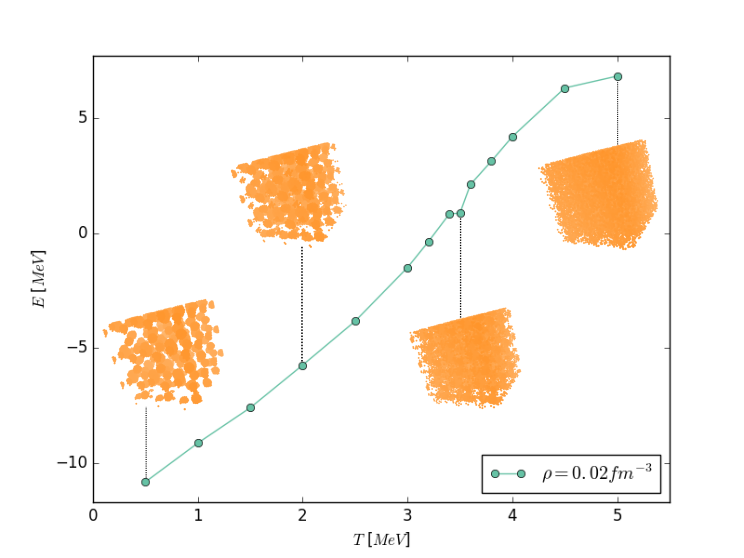
\includegraphics[trim = 5mm 0mm 10mm 5mm, clip, width=0.48\textwidth]{NM/EvsT_noquis.png}
	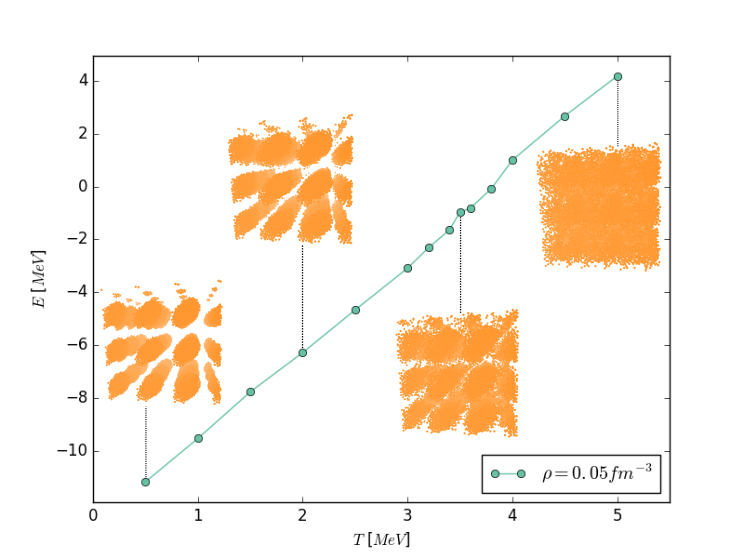
\includegraphics[trim = 5mm 0mm 10mm 5mm, clip, width=0.48\textwidth]{NM/EvsT_fideos.png}
	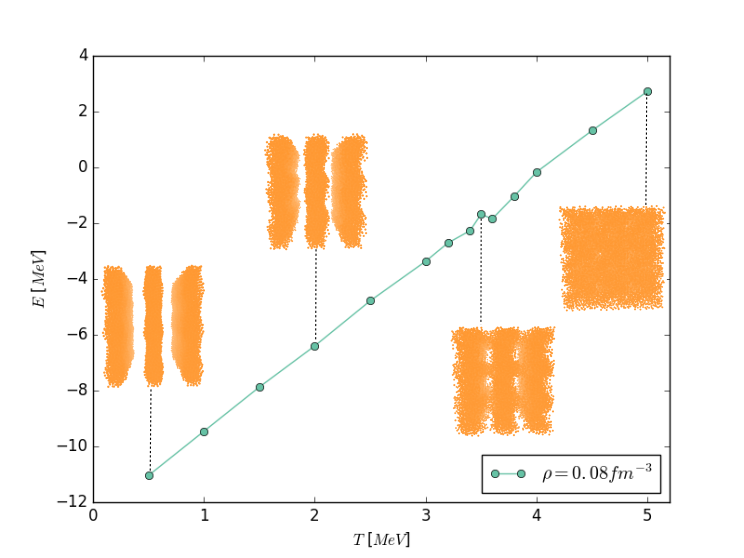
\includegraphics[trim = 5mm 0mm 10mm 5mm, clip, width=0.48\textwidth]{NM/EvsT_lasagna.png}
	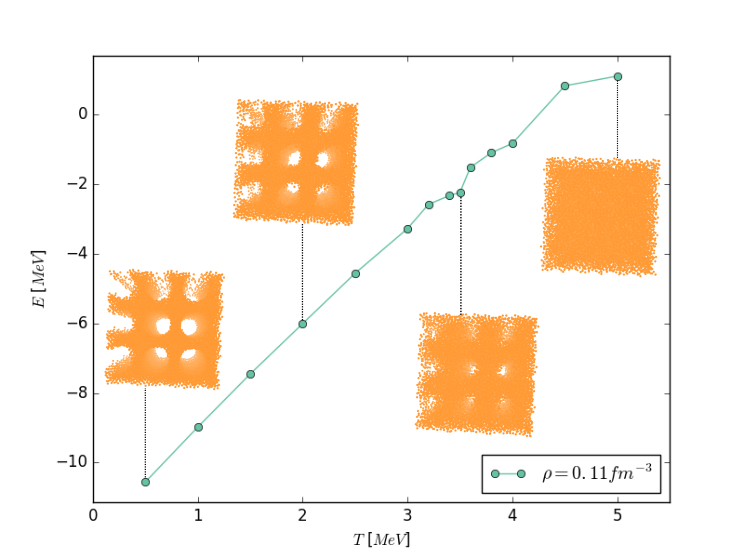
\includegraphics[trim = 5mm 0mm 10mm 5mm, clip, width=0.48\textwidth]{NM/EvsT_tuneles.png}
	\caption{Curvas calóricas para las densidades representando un tipo de pasta particular; ñoquis, spaghettis, lasagna y tuneles.
	La formación de todas ellas ocurre para $3\text{MeV}\leq T\leq4\text{MeV}$.}
	\label{fig:EvsT_pastas}
\end{figure}

En todos los casos, la pasta se originó alrededor de $T=3.5$MeV donde puede apreciarse una región de inestabilidad en los valores de $E$.
Sin embargo, es ciertamente llamativo que no exista salto en la energía entre el estado fundamental de la pasta en $T=0.5$MeV.

La totalidad de las curvas calóricas pueden apreciarse en la \textbf{Figura \ref{fig:Evsrho_QCNMx0,5}}, donde vemos una cierta convergencia para $T\leq 2$MeV.
Para $T=5$MeV, las energías resultan decrecientes en $\rho$ pero a medida que $T$ aumenta alcanzan una región de transición entre $T=3$MeV y $T=4$MeV.
Para $T\leq2$MeV, las curvas parecen converger a una misma pendiente, lo cual coincide en la \textbf{Figura \ref{fig:EvsT_pastas}} con la formación de pastas bien definidas. 

\begin{figure}[H]
	\centering
	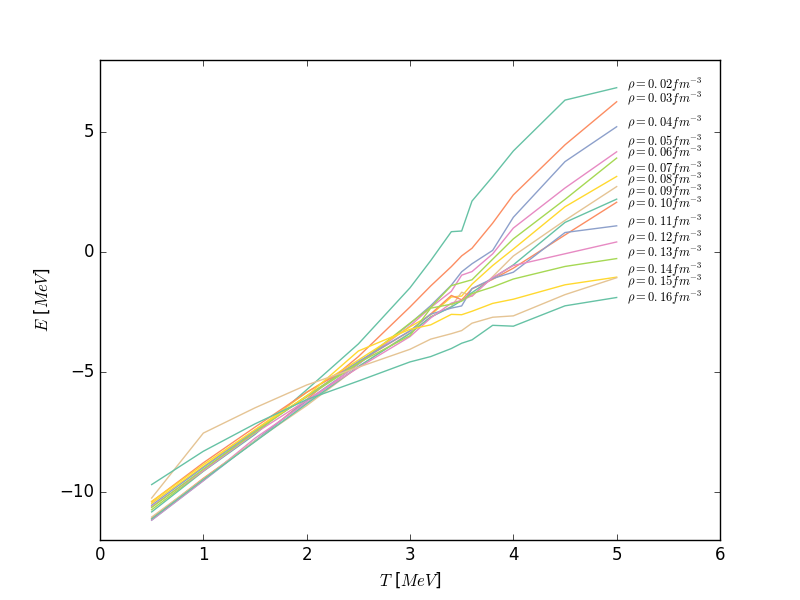
\includegraphics[width=0.9\textwidth]{NM/EvsT_full.png}
	\caption{Curvas calóricas para las distintas densidades. 
	Aunque inicialmente las energías resultan decrecientes en $\rho$, terminan convergiendo para $T\leq 2$MeV.}
	\label{fig:EvsT_QCNMx0,5}
\end{figure}

Este cambio de comportamiento con la temperatura puede apreciarse en la \textbf{Figura \ref{fig:Evsrho_QCNMx0,5}}, donde vemos la curva $E(\rho)$ para  las distintas temperaturas del sistema.
En gris marcamos la región en la que ocurre la aparición de las pastas para la mayor parte de las densidades; correspondiente a $3$MeV$\leq T\leq4$MeV.
Para los valores de $\rho\sim 0.14$fm$^{-3}$ más cercanos a la desaparición de las pastas, esta franja se corre a temperaturas más bajas. 
Es justamente luego de esta transición en $T\sim 3.5$MeV que las curvas $E(\rho)$ pasan de decrecientes a cuasi-constantes.

\begin{figure}[H]
	\centering
	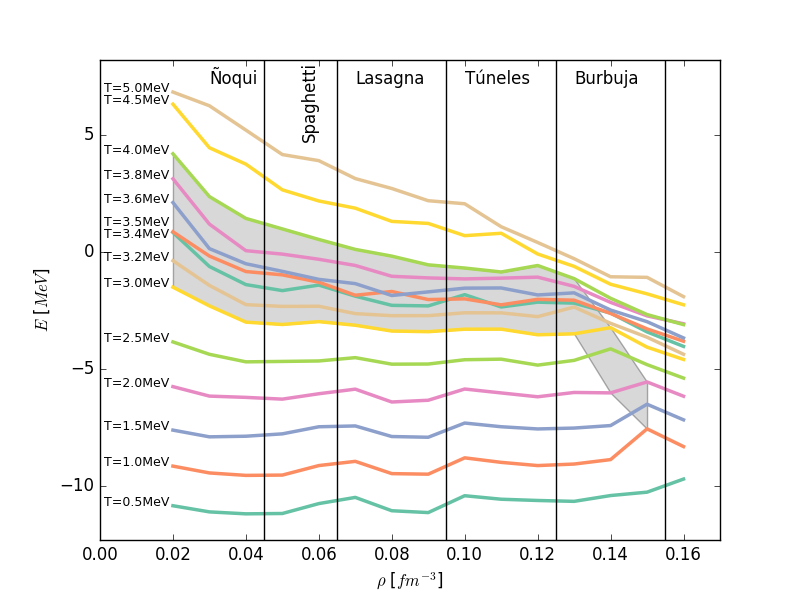
\includegraphics[width=0.9\textwidth]{NM/Evsrho_full.png}
	\caption{Curvas $E$ vs $\rho$ para las distintas temperaturas. 
	La región gris marca el rango de temperaturas en que ocurre la formación de las pastas.
	Es allí también donde se da la transición entre la curva $E$ vs $\rho$ decreciente y la cuasi-constante.
	También se encuentran marcadas con líneas verticales las regiones de densidades correspondientes a cada pasta.}
	\label{fig:Evsrho_QCNMx0,5}
\end{figure}

Es también llamativo comparando las \textbf{Figuras \ref{fig:Evsrho_QCNMx1}} y \textbf{\ref{fig:Evsrho_QCNMx0,5}} podemos observar que las pastas correspondientes a los distintos rangos de densidades
no parecen verse muy afectados por la reducción de $V_o$. 
La única excepción a esto es la región de burbuja, que al reducir el $V_o$ aumentó a costa de la región de túneles. 
Además, la densidad de transición de pasta a gas se da ahora para $\rho \approx 0.16$fm$^{-3}$, un valor levemente menor al anterior. 
Ciertamente, la forma cóncava de la \textbf{Figura \ref{fig:Evsrho_QCNMx1}} se pierde por completo, por lo que el sistema no parece tener un mínimo claro.


\newpage

\section{Apéndice}
 \subsection{Distribución de Boltzmann}{\label{ap:boltzmann}}

La distribución de Boltzmann se da para todos los sistemas (interactuantes o no) de partículas distinguibles (o clásicas) cuyos potenciales sean independientes de los momentos.
Estos Hamiltoneanos tienen la forma
\[ H(\mathbf{q}_1,..,\mathbf{q}_N,\mathbf{p}_1,..,\mathbf{p}_N) = \sum_{i=1}^N \frac{p_i^2}{2m_i} + U(\mathbf{q}_1,..,\mathbf{q}_N)\]
donde $p_i = |\mathbf{p}_i|$ es el modulo del momento.

Sabiendo que los ensambles son equivalentes en el límite termodinámico, haremos este desarrollo en ensamble canónico por simplicidad.
En este ensamble, la (densidad de) probabilidad de un dado microestado $x=(\mathbf{q}_1,..,\mathbf{q}_N,\mathbf{p}_1,..,\mathbf{p}_N)$ está definida por

\[ P(x) = \frac{e^{-\beta H(\mathbf{q}_1,..,\mathbf{q}_N,\mathbf{p}_1,..,\mathbf{p}_N)}}{\int e^{-\beta H} d^{3N}qd^{3N}p} \]

Aprovechando la forma del Hamiltoneano, la integral del denominador puede factorizarse

\begin{align*}
\int e^{-\beta H} d^{3N}qd^{3N}p &= \int e^{-\beta \left( \sum_i p_i^2/2m_i + U(\mathbf{q}_1,..,\mathbf{q}_N)\right)} d^{3N}qd^{3N}p \\
&= \left(\prod_{i=1}^N\int e^{-\beta\frac{p^2}{2m_i}} d^{3}p\right) \int e^{-\beta U(\mathbf{q}_1,..,\mathbf{q}_N)} d^{3N}q
\end{align*}

Podemos entonces preguntarnos cual es la probabilidad de que una dada partícula $i$ tenga momento $\mathbf{p}_i$.
Esta probabilidad $f_i(\mathbf{p}_i)$ se obtiene integrando sobre todos los posibles estados de las demás partículas y sobre la posición $\mathbf{q}_i$ de la partícula $i$.
Analogamente a la cuenta anterior, vemos que esto arroja

\[ f_i(\mathbf{p}_i) = e^{-\beta\frac{p_i^2}{2m}}\frac{\left(\prod_{j=1, j\neq i}^N\int e^{-\beta\frac{p^2}{2m_j}} d^{3}p\right) \int e^{-\beta U(\mathbf{q}_1,..,\mathbf{q}_N)} d^{3N}q}
{\left(\prod_{j=1}^N\int e^{-\beta\frac{p^2}{2m_j}} d^{3}p\right) \int e^{-\beta U(\mathbf{q}_1,..,\mathbf{q}_N)} d^{3N}q}
= \frac{e^{-\beta\frac{p_i^2}{2m_i}}}{\int e^{-\beta\frac{p^2}{2m_i}} d^3p} \]

Efectuando la integral del denominador, obtenemos finalmente la probabilidad de un dado impulso $\mathbf{p}_i$.
\begin{equation}{\label{eq:dist_MB_imp}}
f_i(\mathbf{p}_i) = \left(\frac{\beta}{2\pi m_i} \right)^{3/2} e^{-\beta\frac{p_i^2}{2m_i}}
\end{equation}
conocida como distribución de Maxwell-Boltzmann.

Dado que esta probabilidad es isótropa, resultaría natural plantearla en función del módulo del impulso para volverla una distribución de una única variable.
Para esto, debemos integrar en todas las posibles direcciones del vector $\mathbf{p}_i$ además de introducir un jacobiano.
Podemos obtener la nueva distribución aprovechando la normalización y realizando el cambio de variables a esféricas
\[1 = \int f_i(\mathbf{p}_i) d^3p = \int_0^\infty\int_0^{4\pi}\left(\frac{\beta}{2\pi m_i} \right)^{3/2} e^{-\beta\frac{p_i^2}{2m_i}} p^2d\Omega dp
= \int_0^\infty 4\pi\left(\frac{\beta}{2\pi m_i} \right)^{3/2} p_i^2 e^{-\beta\frac{p_i^2}{2m_i}} dp_i\]
por lo que la probabilidad de que la $i$-esima partícula tenga un momento con módulo $p$ es
\[ f_i(p) = 4\pi\left(\frac{\beta}{2\pi m_i} \right)^{3/2} p^2 e^{-\beta\frac{p^2}{2m_i}} \]

Sin embargo, si todas las partículas son diferentes (por ejemplo, tienen masas $m_i$ diferentes) esta distribución tiene poco valor estadístico, pues no nos otorga información
del sistema en su totalidad.
Sin embargo, analizar la probabilidad de que la partícula tenga una dada energía cinética $\varepsilon = p^2/2m_i$ permitirá independizarnos de la masa.
Analogamente a lo anterior, planteamos normalización y utilizamos el cambio de variables $2m_i\varepsilon = p^2$ con $d\varepsilon = pdp/m = \sqrt{2m\varepsilon}dp/m$

\[ 1 = \int_0^\infty f_i(p) dp = \int_0^\infty 4\pi\left(\frac{\beta}{2\pi m_i} \right)^{3/2} e^{-\beta\varepsilon} 2m_i\varepsilon\frac{m_i}{\sqrt{2m_i\varepsilon}} d\varepsilon
= \int_0^\infty 2\pi\left(\frac{\beta}{2\pi m_i} \right)^{3/2} e^{-\beta\varepsilon} (2m_i)^{3/2}\sqrt{\varepsilon} d\varepsilon \]

Por lo tanto, la probabilidad de que la $i$-esima partícula tenga una dada energía cinética $\varepsilon$ es identicamente igual para todas las partículas
\begin{equation}
 f(\varepsilon) = \sqrt{\frac{4\beta^3\varepsilon}{\pi}}e^{-\beta\varepsilon}
\end{equation}
y por lo tanto nos permite obtener una propiedad global del sistema.
Si cada partícula tiene probabilidad $f(\varepsilon)d\varepsilon$ de tener energía cinética $\varepsilon$, entonces la cantidad de partículas con esa energía cinética es $Nf(\varepsilon)d\varepsilon$.
Esta es la distribución de energía cinética del sistema.



\subsection{Cálculo de las funciones de Fermi}

En esta sección, hablaremos del método utilizado para computar las $f_\nu(z)$ con especial interés en el caso $\nu=3/2$ que aparece al buscar $\mu(N,V,T)$
y, en menor medida, el caso $\nu=5/2$ asociado a la presión.

Como dijimos, las funciones de Fermi están definidas según su forma integral, pero pueden expresarse como una serie alternada
\begin{equation}{\label{eq:fermi_func_serie}}
 f_\nu(z) \equiv \frac{1}{\Gamma(\nu)}\int_0^\infty \frac{x^{\nu-1}}{z^{-1}e^x+1} dx = \sum_{l\geq 1} (-1)^{l+1}\frac{z^l}{l^\nu}
\end{equation}
cuya convergencia resulta lenta para $z$ de orden 1 o mayor.
Sin embargo, para toda $f_\nu(z)$ existirá algún $z_\nu < 1$ que nos asegure una convergencia veloz de las sumas parciales
\[ f_\nu(z) \approx \sum_{l=1}^{m} (-1)^{l+1}\frac{z^l}{l^\nu}\]
para $z\leq z_\nu < 1$.
Esto se debe a que podemos acortar burdamente el error por
\[ \left|f_\nu(z) - \sum_{l=1}^{m}(-1)^{l+1}\frac{z^l}{l^\nu}\right| \leq \sum_{l=m+1}^\infty z^l = z^{m+1}\sum_{l=0}^\infty z^l = z^{m+1} \frac{1}{1-z} \]
donde usamos $z\leq z_\nu < 1$ para resolver la suma geométrica.

Es de esta cota de donde obtendremos el $z_\nu$ que nos asegure un error relativo tolerable.
Por ejemplo, para $m=20$ y $\nu = 3/2$, podemos aproximar $f_\nu(z)$ para $z\leq z_\nu = 0.65$ con sumas parciales cuyo error relativo está acotado por
\[\frac{|f_\nu(z) - \sum_{l=1}^{m}(-1)^{l+1}\frac{z^l}{l^\nu}|}{f_\nu(z)} \leq 10^{-3} = 0.1\%\]

Este error es suficientemente bajo como para afirmar que el método es preciso.
Sin embargo, para $z = 0.75$, el error relativo ya escala a un $2\%$ y para $z=0.8$ al $10\%$, por lo que resulta necesario mejorar el método.
Una forma de lograr esto sería aumentando el $m$ de las sumas parciales, pero esto conlleva el problema inherente de que los sumandos son estrictamente crecientes en módulo para $z\geq 1$.
Eventualmente, estos valores pueden ser suficientemente grandes como para incurrir en \texttt{overflows} o cancelaciones catastróficas.

\subsubsection{Algoritmo de Wynn}

Dado que la expresión de las $f_\nu(z)$ como serie de potencias resulta problemática para $z\geq 1$, podemos recurrir a otras formas.
Una de estas es la aproximación de Padé por una función racional (cociente de polinomios)
\[ [L/M]_{f_\nu}(z) \equiv \frac{P_L(z)}{Q_M(z)} \approx f_\nu(z) \]
donde $P_L(z)$ y $Q_M(z)$ son polinomios de grado $L$ y $M$, respectivamente.
Estos polinomios no nos interesan dado que utilizaremos el \textit{algoritmo $\epsilon$ de Wynn} para obtener las aproximaciones diagonales $[p/p]_{f_\nu}(z) = \epsilon(0, 2p)$
donde $\epsilon(n,m)$ está definido recursivamente según
\begin{align*}
 &\epsilon(n, -1) = 0 \\
 &\epsilon(n, 0) = \sum_{l=0}^{n} c_lz^l \\
 &\epsilon(n, m+1) = \epsilon(n+1,m-1) + \frac{1}{\epsilon(n+1,m) - \epsilon(n,m)}
\end{align*}
que, para el caso de las $f_\nu(z)$, son $c_0 = 0$ y $c_l=(-1)^{l+1}/l^\nu$ para $l\geq1$.

Para facilitar la visualización, suelen organizarse los $\epsilon$ en una tabla de doble entrada $n$ y $m$ como se muestra en la \textbf{Figura \ref{fig:wynn_esquema}}.
Allí puede verse claramente que $\epsilon$ deben conocerse para computar $\epsilon(n,m)$.
En particular, en la \textbf{Figura \ref{fig:wynn_ejemplo}} puede verse que (dado que $\epsilon(n,-1)=0$) para computar la aproximación $[p/p]$ basta con computar los $\epsilon(n,m)$ con $0\leq n\leq 2p-m$ y $m\leq 2p$.
Esto corresponde a la mitad superior de la antidiagonal, por lo que la cantidad de cómputos es $(2p)^2/2$.

\begin{figure}[H]
	\centering
	\subfigure[Recurrencia entre elementos]{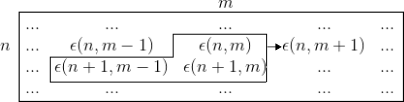
\includegraphics[width=0.26\columnwidth]{apendice/esquema_wynn.png}{\label{fig:wynn_esquema}}}
	\hspace{0.05\columnwidth}
	\subfigure[Ejemplo del cómputo para el caso $p=1$]{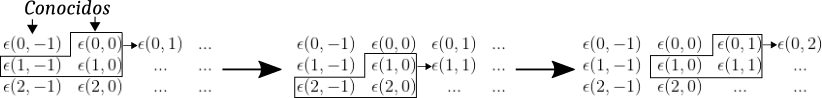
\includegraphics[clip, width=0.68\columnwidth]{apendice/ejemplo_wynn.png}{\label{fig:wynn_ejemplo}}}
	\caption{Arreglo de los coeficientes $\epsilon$ en una tabla para facilitar su cómputo}
	\label{fig:wynn}
\end{figure}

Para una serie de Padé $[p/p]$, el error es $O(z^{2p})$, por lo que tomando $p=10$ podemos obtener un orden similar al de la serie truncada.
Por lo tanto, resultaría razonable utilizar el algoritmo de Wynn para $z\geq z_\nu$, donde (en el caso $\nu=3/2$) empalma con el método de serie truncada con un error
relativo de $\sim10^{-6}$ más que aceptable.

Aunque, en general, las $f_\nu(z)$ no poseen una expresión analítica contra la que podamos comparar la eficacia del algoritmo, el caso particular $\nu=1$ si tiene
expresión analítica: $f_1(z) = \log(z+1)$.
A modo de ejemplo, en la \textbf{Figura \ref{fig:ej_wynn_log}} las aproximaciones a $f_1(z) = \log(z+1)$ mediante el algoritmo de Wynn y sus errores relativos.
Usamos como valor ``exacto'' el arrojado por la función \texttt{log} del paquete \texttt{numpy} de \texttt{Python}.
Puede verse que en el rango $0\leq z\leq 20$, la aproximación con $2p=20$ resulta indistinguible del exacto.

\begin{figure}[H]
	\centering
	\subfigure[Valor absoluto]{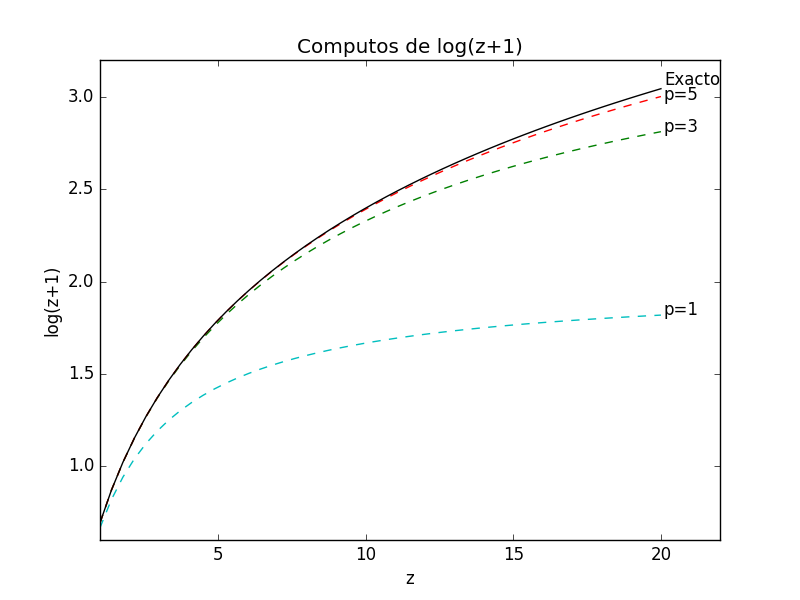
\includegraphics[width=0.4\columnwidth]{apendice/ejemplo_wynn_log.png}}
	\hspace{0.05\columnwidth}
	\subfigure[Error relativo]{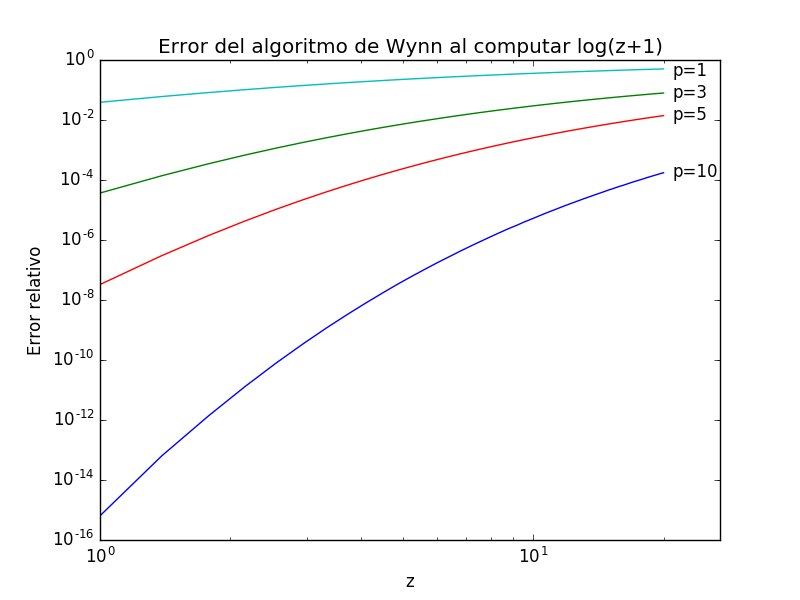
\includegraphics[width=0.4\columnwidth]{apendice/ejemplo_wynn_log_error.png}}
	\caption{Aproximaciones del método de Wynn a la función $f_1(z) = \log(z+1)$, calculada usando el paquete \texttt{numpy} de \texttt{Python}.
	Podemos ver que rapidamente converge a la función para $p=10$, que resulta indistinguible de la exacta.}
	\label{fig:ej_wynn_log}
\end{figure}

Sin embargo, uno podría preguntarse que nos impide utilizar el algoritmo de Wynn en todo el rango de $z$.
Para $z$ pequeño, dado que las sumas parciales de $\epsilon(n,0)$ convergen rapidamente, la resta que aparece en el demonimador de la definición recursiva de
$\epsilon(n, m+1)$ tiende a ser menor al número de máquina, transformándolo en una división por $0$.

Para $z$ suficientemente grande, las sumas parciales de $\epsilon(n,0)$ resultan dominadas por el término $z^n$, con $0\leq n\leq 2p$ y $p\sim 10$.
Por lo tanto, los $\epsilon(n,0)$ se vuelven muy grandes y problemáticos para trabajar para $z\geq 100$.
Para el caso $\nu=3/2$, observamos las primeras inestabilidades para $z\approx 30$.


\subsubsection{Aproximación de Sommerfeld y forma final}

Para $z$ grande, necesitamos otra forma de computar la $f_\nu(z)$.
Surge la pregunta entonces: ¿existe un $z_m$ suficientemente grande para el cual nos baste conocer $f_\nu(z)$ para $z\leq z_m$?
Esta pregunta surge de recordar el objetivo de partida: encontrar el $z$ que cumple $f_\nu(z)=\frac{N\lambda^3}{gV}\equiv \alpha$.
A priori, $\alpha$ no está acotado superiormente, por lo que necesitamos conocer los $z$ para los cuales $f_\nu(z)\to\infty$.
En particular, estamos interesados en que tanto debemos aumentar $z$ para que $f_\nu(z)$ aumente una dada cantidad.

Para esto, utilizamos el conocido lema de Sommerfeld que nos permite aproximar
\begin{equation}{\label{eq:sommerfeld}}
 \int_0^\infty \frac{\Phi(x)}{e^{x-\eta}+1}dx = \int_0^\eta \Phi(x) dx + \frac{\pi^2}{6}\left( \frac{d\Phi}{dx} \right)\Bigg|_{x=\eta} +
 \frac{7\pi^4}{360}\left( \frac{d^3\Phi}{dx^3} \right)\Bigg|_{x=\eta} + ...
\end{equation}

Para el caso de $f_\nu(z)$, podemos usar este lema con $\Phi(x) = x^{\nu-1}/\Gamma(\nu)$ y $z = e^{\eta}$ (o $\eta = \log z$), obteniendo
\begin{equation}{\label{eq:dirac_sommerfeld}}
f_\nu(z) = \frac{1}{\Gamma(\nu)}\left[ \frac{(\log z)^\nu}{\nu} + \frac{\pi^2}{6}(\nu - 1)(\log z)^{\nu-2} + \frac{7\pi^4}{360}(\nu - 1)(\nu - 2)(\nu - 3)(\log z)^{\nu - 4}
+ O((\log z)^{\nu-6})  \right]
\end{equation}

Esto nos dice que para $z$ suficientemente grande, las $f_\nu(z)$ se comportan como potencias del logaritmo de $z$.
Por lo tanto, el crecimiento de $f_\nu(z)$ es considerablemente lento y obtener valores grandes de $f_\nu(z)$ exige valores muchisimo mayores de $z$.
Por ejemplo, utilizar la aproximación de Sommerfeld para resolver $f_{3/2}(z) = 30$ arroja un $z\approx 10^5$.

Para los valores de $z\geq 20$, utilizamos la aproximación \eqref{eq:dirac_sommerfeld} que empalma en $z=20$ con el algoritmo de Wynn con un error relativo de
$\sim10^{-3}$ aceptable (para $\nu=3/2$).

La ventaja de esto es que para $z\geq 20$ tenemos un método explícito y veloz para evaluar $f_{3/2}(z)$, por lo que podemos utilizar algún método para hallar la
raíz de $g(z) = 0 = f_{3/2}(z) - N\lambda^3/gV$ (en nuestro caso, bisecciones).
Por otro lado, para $0\leq z\leq 20$ construimos una Look-Up Table de $\sim 2500$ puntos, interpolando para obtener los valores de $f_\nu(z)$.
En resumen

\[  \left(\nu = \frac{3}{2}\right) \qquad
 \left\{\begin{matrix}
  0 \leq z \leq 20 & \text{Look-Up Table: } \left\{\begin{matrix}
		    0 \leq z \leq 0.65 & \text{Sumas parciales: } f_{3/2}(z) = \sum_{l=1}^{20} (-1)^{l+1} z^l/l^\nu \\
		    0.65 \leq z \leq 20 & \text{Wynn: } \quad f_{3/2}(z) = \epsilon(0,20)
		    \end{matrix}\right. \\
 z\geq 20 & \text{Sommerfeld: } \qquad \qquad f_{3/2}(z) = \frac{4(\log z)^{3/2}}{3\pi^{1/2}}\left[ 1 + \frac{\pi^2}{8}(\log z)^{-2} - \frac{7\pi^4}{384}(\log z)^{-4}  \right]
 \end{matrix} \right.
\]

Para calcular las $f_{5/2}(z)$ asociadas a la presión, debimos aumentar el $z_\nu$ hasta $0.75$ manteniendo el límite inferior de Sommerfeld.
Esta aproximación de la $f_{5/2}(z)$ tiene una calidad similar a la de $f_{3/2}(z)$, como se ve en la \textbf{Figura \ref{fig:f32_f52}}.

\begin{figure}[H]
	\centering
	\subfigure[Función $f_{3/2}(z)$ utilizada para obtener $\mu(N,V,T)$]{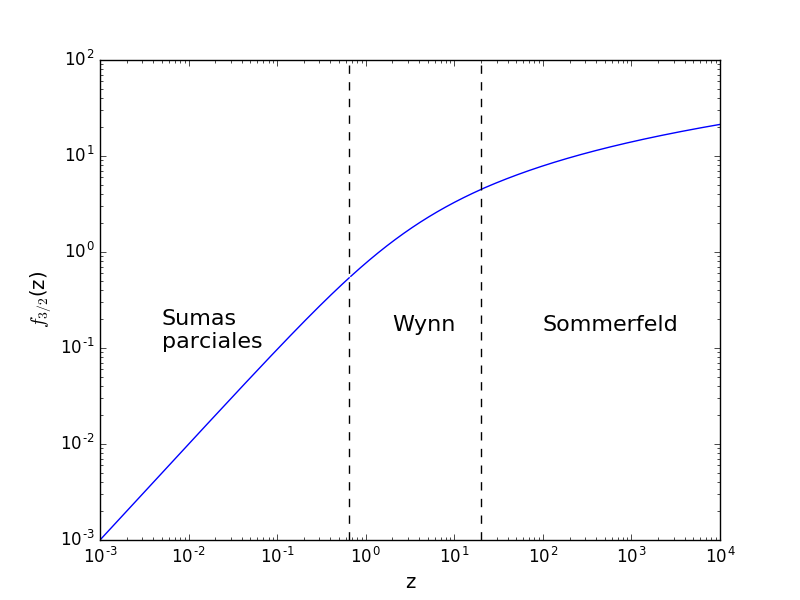
\includegraphics[width=0.4\columnwidth]{apendice/F32.png}}
	\hspace{0.05\columnwidth}
	\subfigure[Función $f_{5/2}(z)$ asociada a la presión del sistema]{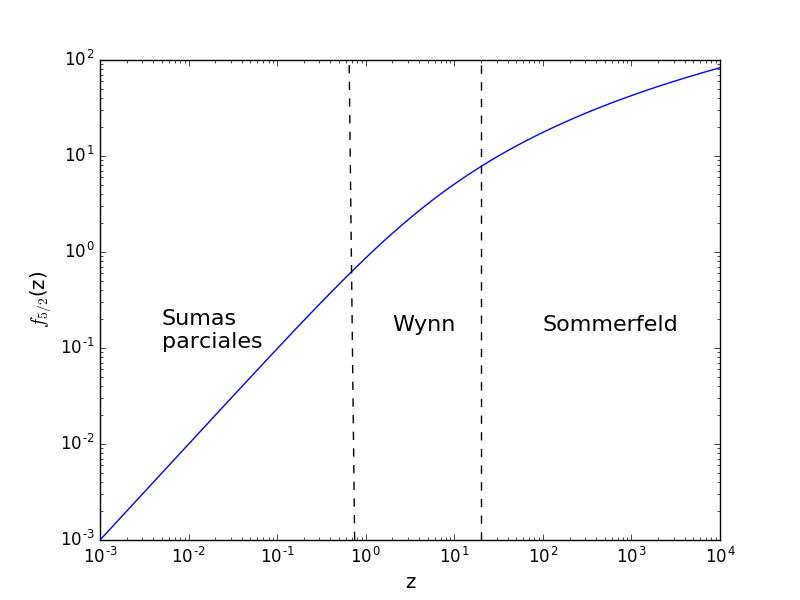
\includegraphics[width=0.4\columnwidth]{apendice/F52.png}}
	\caption{Forma final de las $f_\nu(z)$ utilizando la separación en 3 métodos: sumas parciales, Wynn y Sommerfeld. Puede verse que empalman correctamente.}
	\label{fig:f32_f52}
\end{figure}



\subsection{Teorema del virial}{\label{ap:teo_virial}}

El teorema del virial es un resultado general para sistemas con $q$ y $p$ acotados que surge tanto de la mecánica clásica como de la mecánica estadística.
Nos concentraremos en la versión de mecánica estadística deducida para el ensamble canónico y aprovechando la equivalencia de ensambles en el límite termodinámico.
En particular, analizaremos los valores medios de los observables
\begin{align*}
\left< \dpart{H}{q_i}q_i \right> = \frac{1}{Z}\int \dpart{H}{q_i}q_i e^{-\beta H} d^{3N}qd^{3N}p  &= -\frac{1}{Z\beta}\int q_i \dpart{}{q_i}\left(e^{-\beta H}\right) d^{3N}qd^{3N}p \\
&= -\frac{1}{Z\beta}\int \left[ \cancel{\dpart{}{q_i}\left(e^{-\beta H} q_i\right)} - e^{-\beta H} \right] d^{3N}qd^{3N}p \\
&= \frac{1}{Z\beta}\int  e^{-\beta H} d^{3N}qd^{3N}p = k_B T
\end{align*}
donde hemos usado que el sistema se encuentra acotado en $q$ para cancelar la integral con la derivada.
Podemos hacer un procedimiento análogo para $p_i$ y así obtener
\begin{equation}{\label{eq:teo_virial_T}}
  \left< \dpart{H}{q_i}q_i \right> = k_B T = \left< \dpart{H}{p_i}p_i \right>
\end{equation}

Utilizando las ecuaciones de Hamilton, podemos deducir de \eqref{eq:teo_virial_T} la conocida versión de la mecánica clásica
(donde ahora $\left< \bullet \right>$ corresponde a valor medio temporal)
\begin{equation}{\label{eq:teo_virial_mec}}
  \left< \dot{q}_ip_i \right> + \left< \dot{p}_iq_i \right> = 0 = \frac{d}{dt}\left< q_ip_i \right>
\end{equation}

Dado que ya tenemos una forma de obtener $T$, resulta natural considerar una fórmula para obtener $P$.
Para esto utilizaremos \ref{eq:teo_virial_mec} separando $\dot{p}_i = F_i = F_i^{int}+F_i^{ext}$ y sumando sobre todas las coordenadas del sistema tal que
\[ 0 = \left< \sum_{i=1}^{3N} \dot{q}_ip_i + F_i^{int}q_i \right> + \left< \sum_{i=1}^{3N}F_i^{ext}q_i \right>  \]
donde vemos que el segundo término corresponde a una especie de trabajo de las fuerzas externas que equivale a $-3PV$\textbf{CITA HAILE, APENDICE B}.
Por lo tanto, la presión resulta
\begin{equation}{\label{eq:teo_virial_P}}
P = \frac{1}{3V}\left< \sum_{i=1}^{3N} \dot{q}_ip_i + F_i^{int}q_i \right>
\end{equation}

Para el caso de un potencial no dependiente de momentos, el primer término de la sumatoria se reduce a la energía cinética.
Sin embargo, para un sistema con interacción como la de Pauli agregará un término de \textit{g\"uerzas}.


\subsection{Integradores no simplécticos: Euler y Runge-Kutta}{\label{sec:no_simp}}

En este apéndice, demostraremos que los métodos de Euler y un Runge-Kutta de orden 2 explícitos no son simplécticos.
Comenzaremos con el método de Euler de esquema
\[ y_{n+1} = y_n + h J^{-1} \nabla H(y_n) \]
cuya derivada respecto de $y_n$ resulta inmediatamente
\[ \dpart{y_{n+1}}{y_n} = 1 + hJ^{-1}\nabla^2H (y_n)\]
\begin{align*}
 \left( \dpart{y_{n+1}}{y_n} \right)^T J \left( \dpart{y_{n+1}}{y_n} \right) &= \left(1 + h\nabla^2 H(y_n)(J^{-1})^T\right) J \left(1 + hJ^{-1}\nabla^2 H(y_n)\right) \\
 &= \left(1 - h\nabla^2 H(y_n)J^{-1}\right) J \left(1 + hJ^{-1}\nabla^2 H(y_n)\right) \\
 &= J - \cancel{h\nabla^2 H(y_n)} + \cancel{h\nabla^2 H(y_n)} - h^2\nabla^2 H(y_n)J^{-1}\nabla^2 H(y_n) \neq J
\end{align*}

Por otro lado, el método Runge-Kutta de orden 2 con esquema
\[ y_{n+1} = y_n + h J^{-1} \nabla H\left(y_n + \frac{h}{2} J^{-1} \nabla H(y_n) \right) \equiv y_n + h J^{-1} \nabla H\left(y_{n+1/2} \right) \]
tiene una derivada respecto de $y_n$ más complicada
\begin{align*}
\dpart{y_{n+1}}{y_n} &=  1 - h\left[ 1 - \frac{h}{2} \nabla^2 H(y_n)J^{-1} \right]\nabla^2H\left(y_n + \frac{h}{2} J^{-1} \nabla H(y_n)J^{-1} \right) \\
&\equiv 1 - h\left[ 1 - \frac{h}{2} \nabla^2 H(y_n)J^{-1} \right]\nabla^2H\left(y_{n+1/2} \right) 
\end{align*}
\begin{align*}
 &\left( \dpart{y_{n+1}}{y_n} \right)^T J \left( \dpart{y_{n+1}}{y_n} \right) = \left( 1 - h\left[ 1 - \frac{h}{2} \nabla^2 H(y_n)J^{-1} \right]\nabla^2H\left(y_{n+1/2} \right)J^{-1} \right) J \\
 &\qquad \qquad \qquad \left(1 + hJ^{-1}\nabla^2H\left(y_{n+1/2} \right)\left[ 1 + \frac{h}{2} J^{-1} \nabla^2 H(y_n) \right] \right)\\
 &= J + \frac{h^2}{2} \nabla^2 H(y_n)\nabla^2H(y_{n+1/2}) + \frac{h^2}{2} \nabla^2H(y_{n+1/2})\nabla^2 H(y_n) -\\
 &h^2\left[ 1 - \frac{h}{2} \nabla^2 H(y_n)J^{-1} \right]\nabla^2H(y_{n+1/2}) J^{-1}\nabla^2H(y_{n+1/2})\left[ 1 + \frac{h}{2} J^{-1} \nabla^2 H(y_n) \right] \\
 &= J + \frac{h^2}{2} \left[ \nabla^2 H(y_n)\nabla^2H(y_{n+1/2}) +  \nabla^2H(y_{n+1/2})\nabla^2 H(y_n) - 2\nabla^2H\left(y_{n+1/2} \right) J^{-1}\nabla^2H(y_{n+1/2}) \right] \\
 & + \frac{h^3}{2} \left[ \nabla^2H(y_{n+1/2}) J^{-1}\nabla^2H(y_{n+1/2})J^{-1} \nabla^2 H(y_n) - \nabla^2 H(y_n)J^{-1}\nabla^2H(y_{n+1/2}) J^{-1}\nabla^2H(y_{n+1/2})\right] \\
 & + \frac{h^4}{4} \nabla^2 H(y_n)J^{-1}\nabla^2H(y_{n+1/2}) J^{-1}\nabla^2H(y_{n+1/2})J^{-1}\nabla^2 H(y_n)
\end{align*}

Para anular los ordenes cuadrático y cúbico, se requiere basicamente $\nabla^2H(y_n) = \nabla^2H(y_{n+1/2})$, pero el término cuártico en $h$ es no nulo.
Por lo tanto, este método RK2 no es simpléctico.

\subsection{Implementación de interacción de Pauli}

El objetivo fue generar un método para implementar el cálculo de las fuerzas totales en un sistema de $N_{part}$ partículas para un potencial dado. 
Esta función \texttt{forces} debía ser tan general como fuese posible para así evitar problemas a la hora de cambiar el potencial. 
Implementamos estas funciones en \texttt{C} y, posteriormente, comparamos su velocidad de ejecución para distintas optimizaciones del compilador: \texttt{O0}, \texttt{O1}, \texttt{O2}, \texttt{O3} y \texttt{Ofast}. 

La opción \texttt{O0} es la opción por default en la que no hay optimizaciones mientras que \texttt{O1} es la opción con optimizaciones elementales. 
Por otro lado, la optimización \texttt{O2} realiza todas las optimizaciones que no envuelven \textit{space-speed tradeoff} (mayor uso de memoria en pos de aumentar la velocidad). La opción \texttt{O3}, en cambio, 
si realiza este tipo de optimizaciones como el inlineado de funciones y la vectorización de ciclos. 
Finalmente, la opción \texttt{Ofast} hace todo esto junto optimizaciones que no son \textit{standard-compliant} como \texttt{-ffast-math}; librería con funciones matemáticas implementadas para tener una mayor 
velocidad pero no necesariamente arrojar resultados con la exactitud apropiada. 

Teniendo estas funciones implementadas de la mejor manera, podríamos compilarlas en una librería dinámica y llamarlas desde \texttt{Python}.
De esta manera, podiamos aprovechar la velocidad de cómputo de \texttt{C} junto con la versatilidad de una sesión interactiva de \texttt{Python}.

Con esto en mente, planteamos 9 posibles implementaciones de la función \texttt{forces} combinando distintos rasgos. 
En todos los casos (excepto el primero), \texttt{forces} llamaba otras funciones para ejecutar el cálculo de la fuerza (\texttt{pair\_force}) o energía (\texttt{pair\_energ}) de interacción entre 2 partículas. 
Los rasgos que modificamos fueron: 

\begin{quote}
\begin{description}
\item[Precalculo:] El pre-cálculo o no de parámetros relevantes para la interacción tanto en la energía como en la fuerza de 2 partículas

\item[Auxiliares:] Separar el cálculo auxiliar en 2 funciones distintas \texttt{pair\_force} y \texttt{pair\_energ} o tener una única función \texttt{pair\_energ\_force}

\item[Modulo:] Que la función auxiliar que calcula la fuerza de interacción devuelva el vector completo (con sus 3 componentes) o solo el módulo.
\end{description}
\end{quote}

Comparamos todas estas funciones con una función \texttt{forces1} sin funciones auxiliares que, en principio, sería la más veloz. Así, fue posible evaluar que tanta velocidad de ejecución se perdía en pos de 
la encapsulación del potencial. 

\subsubsection{Estabilización del tiempo de ejecución}

Preliminarmente, buscamos el valor de $N_{part}$ a partir del cual el tiempo de ejecución resultaba $\tau\sim N_{part}^2$ dado que la cantidad de interacciones que \texttt{forces} calculaba es 
$N_{part}(N_{part}-1)/2\sim N_{part}^2$, bajo la hipótesis de que el tiempo de cómputo de la interacción entre 2 partículas es independiente de sus posiciones. 
Para asegurar esto último, evitamos la aplicación de un radio de corte $r_c$ para el potencial (en este caso Morse) que lo anule $\forall r\geq r_c$.

Esto lo hicimos calculando el tiempo que tomaba computar $N_{iter}$ veces las fuerzas de un sistema de $N_{part}$ partículas. 
Los resultados se muestran en la \textbf{Figura \ref{fig:TvsNpart}} y permiten extrapolar que para simulaciones cuya duración sea mayor a $1ms$ o $N_{part}\geq200$, el comportamiento es cuadrático en $N_{part}$.

\begin{figure}[h]
	\centering
	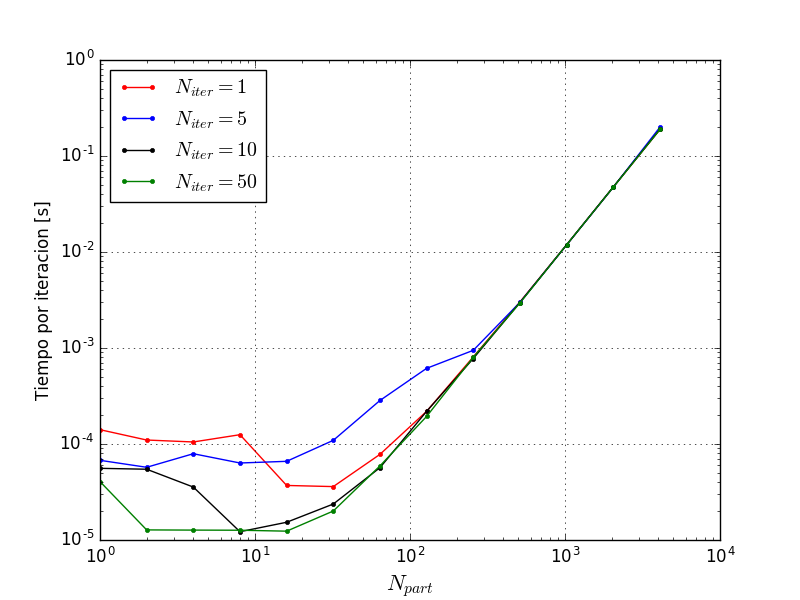
\includegraphics[width=0.65\columnwidth]{apendice/implementacion/Estabilizacion_Npart.png}
	\caption{Tiempo de ejecución de $N_{iter}$ \texttt{forces} para $N_{part}$ partículas. Para $N_{part}>200$ el tiempo ya es polinómico (cuadrático) para todo $N_{iter}$. 
	Esto se condice con simulaciones cuya duración supera $1ms$}
	\label{fig:TvsNpart}
\end{figure}

\subsubsection{Comparación: Potencial de Morse}

El primer potencial que implementamos fue el de Morse
\[ V_{M} (r) = D\left[1-e^{-\alpha (r-r_{eq})}\right]^2\]
dado que su cómputo es muy similar al de Pauli, exigiendo el cálculo de una exponencial.

Realizamos 9 implementaciones del mismo, destacando la implementación 1 por ser la más directa y las funciones 5 y 9 por su mayor portabilidad, además de que devolvian el módulo de fuerza.

\begin{quote}
\begin{description}
\item[1] Sin funciones auxiliares.
\item[5] Dos funciones, con parámetros precalculados, devuelve modulo de fuerza.
\item[9] Dos funciones, sin parámetros precalculados, devuelve modulo de fuerza (encapsula totalmente el potencial).
\end{description}
\end{quote}

\begin{multicols}{3}
\begin{lstlisting}
float forces1(...){
	...
	for(i=0;i<N;i++){
		for(j=i+1;j<N;j++){
			...
			calculo 
			de fuerza
			...
			calculo 
			de energia
			...
		}	
	}
}
\end{lstlisting}
\columnbreak
\begin{lstlisting}
float forces5(...){
	...
	for(i=0;i<N;i++){
		for(j=i+1;j<N;j++){
			...
			precalculo de parametros
			...
			pair_force(params,..)
			pair_energ(params,..)
		}	
		...
	}
	...
}

float pair_force(params,..){
...
}

float pair_energ(params,..){
...
}
\end{lstlisting}

\columnbreak
\begin{lstlisting}
float forces9(...){
	...
	for(i=0;i<N;i++){
		for(j=i+1;j<N;j++){
			pair_force(...)
			pair_energ(...)
		}	
		...
	}
	...
}

float pair_force(..){
	calculo de 
	parametros
	...
}

float pair_energ(..){
	calculo de 
	parametros
	...
}

\end{lstlisting}

\end{multicols}


Esta portabilidad permite usar las 2 funciones auxiliares como \textit{test} directamente desde \texttt{Python} y aprovechan que el vector dirección de la fuerza es independiente del potencial. 
Las demás funciones son:

\begin{quote}
\begin{description}
\item[2 y 3] Única función auxiliar \texttt{pair\_energ\_force} con y sin parámetros precalculados.
\item[4] Como \texttt{forces5} pero devolviendo el vector completo
\item[6] Como \texttt{forces9} pero con algunos parámetros precalculados (no todos).
\item[7 y 8] Versiones de \texttt{forces6} y \texttt{forces9} con una única función auxiliar \texttt{pair\_energ\_force}.
\end{description}
\end{quote}

Compilando con las distintas optimizaciones \texttt{O} corrimos las simulaciones para sistemas con $N_{part}=216$. 
Calculamos el tiempo por par de interacción mediante 
\[ \tau_{par}=\frac{2\tau}{N_{part}(N_{part}-1)} =\frac{\tau}{23220} \]
donde $\tau$ era el tiempo total de duración de la simulación, obtenido mediante estadística sobre $1000$ corridas. 
Los resultados pueden apreciarse en la \textbf{Figura \ref{fig:CompTodas}}.

\begin{figure}[h]
	\centering
	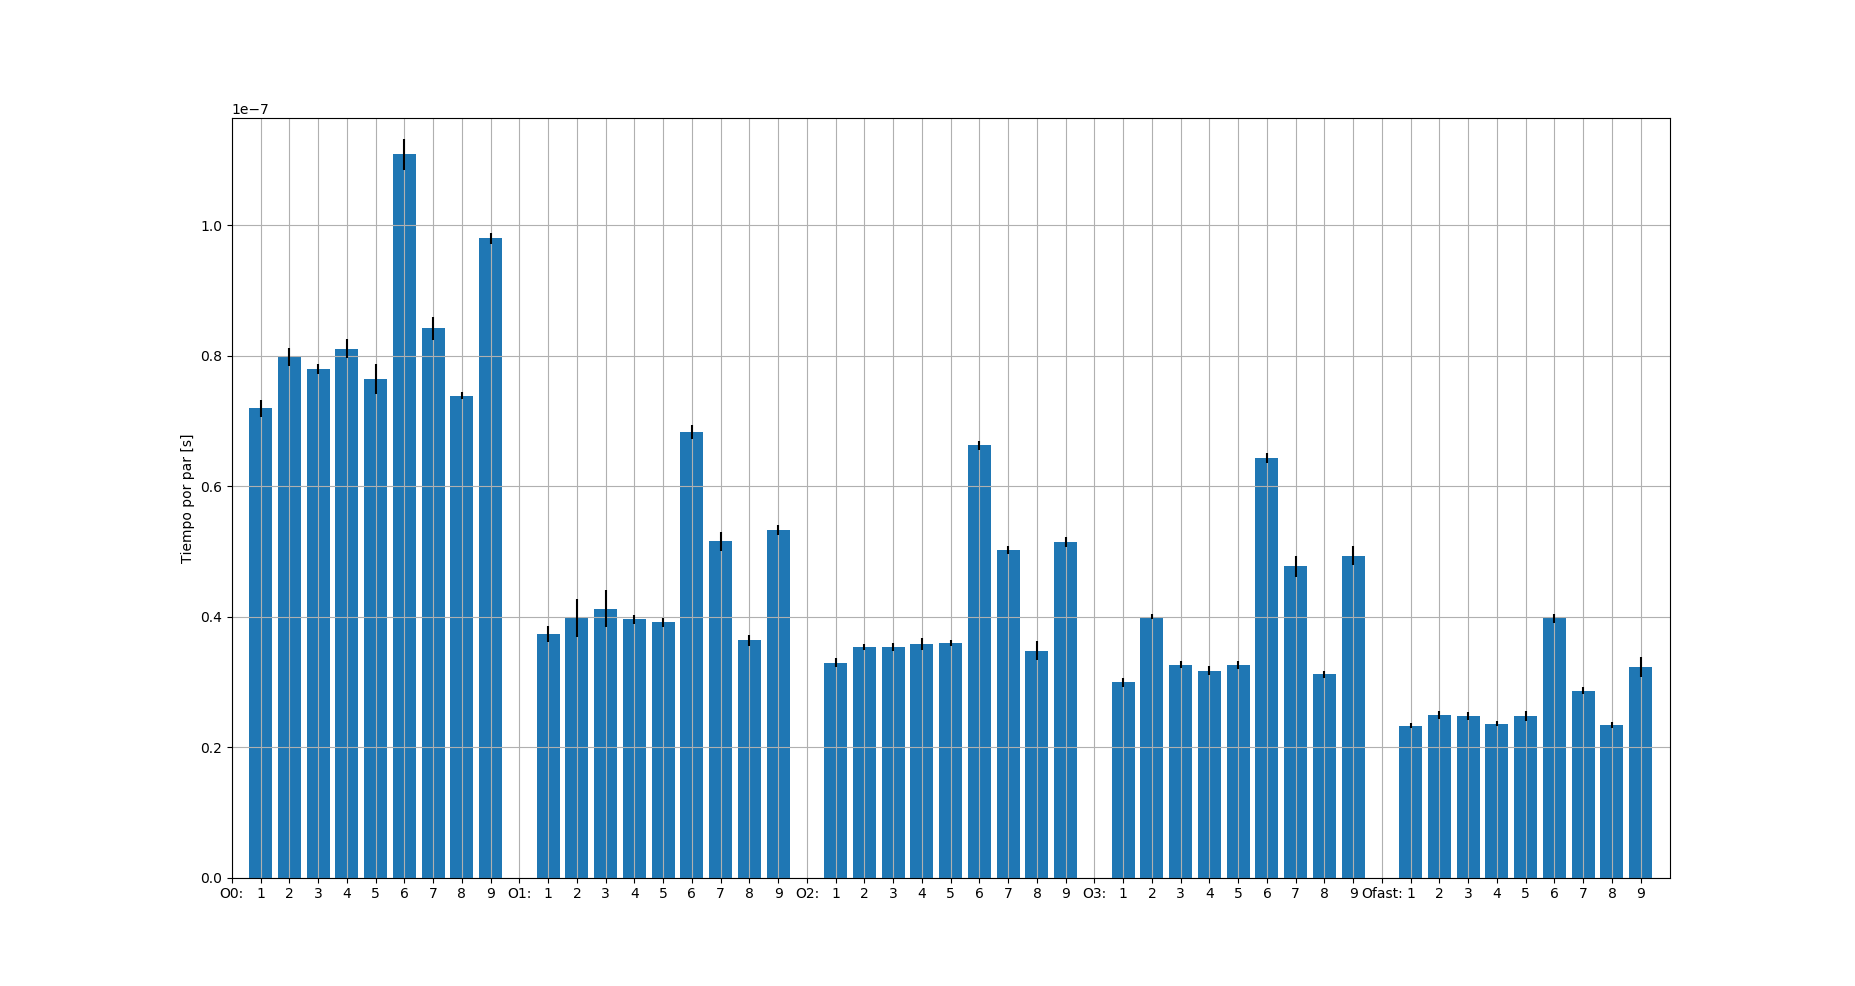
\includegraphics[trim = 40mm 20mm 40mm 20mm, clip, width=\columnwidth]{apendice/implementacion/Comp_tiempos_morse_todos.png}
	\caption{Comparación de tiempos para las distintas implementaciones del potencial de morse. 
	La tendencia decreciente de \texttt{O0} a \texttt{Ofast} es clara, excepto excepciones puntuales de \texttt{O2} a \texttt{O3}.}
	\label{fig:CompTodas}
\end{figure}

En general, puede verse una tendencia decreciente a medida que se pasa de \texttt{O0} a \texttt{Ofast}, lo cual resulta esperable. 
Sin embargo, algunas excepciones notables se dan en el paso de \texttt{O2} a \texttt{O3}.

De mayor interés es notar que el compilador \texttt{Ofast} logra que las implementaciones 2, 3, 4 y 5 tengan diferencias menores al $5\%$ entre si y respecto de la implementación 1, 
volviéndolas virtualmente equivalentes.  
Por tanto, estas 4 implementaciones bien pueden ser reemplazadas unicamente por 5, que resulta más portable como dijimos previamente.

Además, viendo que las implementaciones 6 y 7 tienen tiempos comparables a 9, resulta razonable reemplazarlas por 9. 
En el caso de \texttt{forces9} es importante aclarar que, al no tener ningún parámetro precalculado, la encapsulación del potencial es completa. 
Desde el punto de vista de la ingeniería de software \texttt{forces9} sería la óptima. 

Por lo tanto, aislamos las funciones \texttt{forces1}, \texttt{forces5} y \texttt{forces9} para cuantificar la pérdida de velocidad en pos de la portabilidad (encapsulación del potencial) y 
se volvieron a correr las simulaciones, obteniendo los resultados de la \textbf{Figura \ref{fig:CompEsp}}

\begin{figure}[h]
	\centering
	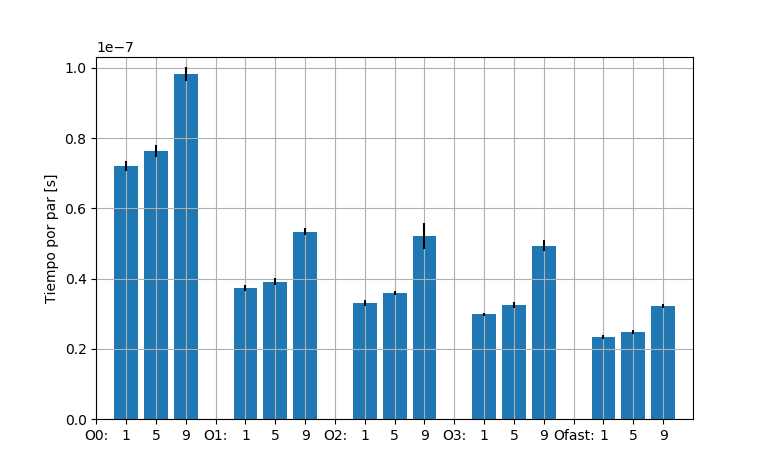
\includegraphics[trim = 10mm 5mm 10mm 5mm, clip, width=0.6\columnwidth]{apendice/implementacion/Comp_tiempos_morse.png}
	\caption{Comparación de las implementaciones de mayor portabilidad (5 y 9) contra la implementación directa 1. 
	Aunque 1 parece equivalente a 5, difiere con 9 en $\sim 40\%$}
	\label{fig:CompEsp}
\end{figure}

Como observamos previamente, la implementación 5 resulta equivalente a la 1 para todos los \texttt{O} (excepto \texttt{O0}). 
Sin embargo, la implementación 9 resulta notoriamente más lenta, con una diferencia relativa respecto a 1 que crece a medida que pasamos de \texttt{O0} a \texttt{Ofast} (donde alcanza un $\sim40\%$). 
Esto último puede deberse a que la separación en 2 funciones obliga a calcular la funcion \texttt{exp} 2  veces, lo cual no ocurre en la implementacion 1 (es directa) ni en la 5 (la exponencial se
pasa como parámetro precalculado). 
Dado que la exponencial no es una función elemental, sus tiempos elevados de calculo pueden causar esta discrepancia.

\subsubsection{Comparación: Potencial de Lennard-Jones}

Con el objetivo de confirmar que la abismal diferencia entre la implementación 9 y la 1 se debe al cálculo de \texttt{exp}, realizamos un análisis similar al anterior para el potencial de Lennard-Jones 
\[ V_{LJ} (r) =  4\varepsilon \left[ \left(\frac{r}{\sigma}\right)^{12} -\left(\frac{r}{\sigma}\right)^{6} \right] \]
que puede calcularse utilizando solamente operaciones algebraicas elementales (multiplicación, suma, resta y división). 
Realizamos las siguientes implementaciones, análogas a 1, 5 y 9 en el caso del potencial de Morse
	
\begin{quote}
\begin{description}
\item[1] Sin funciones auxiliares.
\item[2] Dos funciones, con parámetros precalculados, devuelve modulo de fuerza.
\item[3] Dos funciones, sin parámetros precalculados, devuelve modulo de fuerza (encapsula totalmente el potencial).
\end{description}
\end{quote}

Análogamente, hicimos corridas con cada optimización \texttt{O}, promediando los tiempos con $1000$ corridas. 
Los resultados se encuentran en la \textbf{Figura \ref{fig:CompEsp_LJ}}, donde puede verse el gran salto entre \texttt{O0} y \texttt{O1}, con sus sucesivos saltos de menor orden. 
En particular, entre \texttt{O3} y \texttt{Ofast} no hay ninguna mejora de velocidad. 
Sin embargo, sigue manteniendose la abismal diferencia entre la implementación 9 y la 1 de un $40\%$.

\begin{figure}[h]
	\centering
	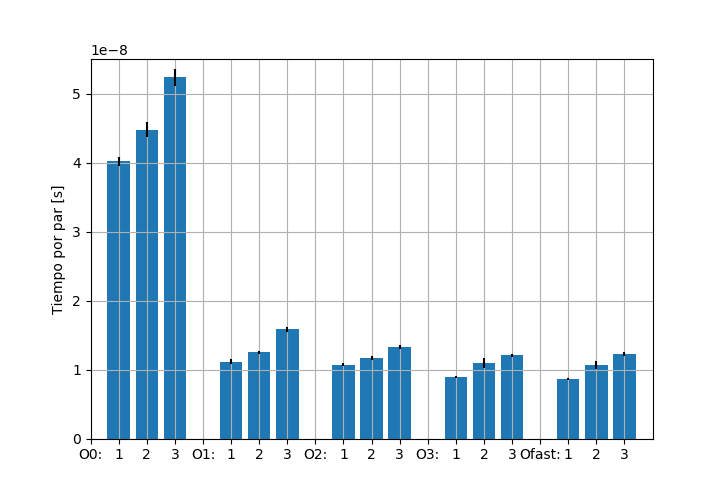
\includegraphics[trim = 10mm 5mm 10mm 5mm, clip, width=0.6\columnwidth]{apendice/implementacion/Comp_tiempos_LJ.png}
	\caption{Comparación de las implementaciones de mayor portabilidad contra la implementación directa 1. 
	A diferencia del caso de Morse, la implementación 2 y 3 resultan notoriamente más lentas que la 1.}
	\label{fig:CompEsp_LJ}
\end{figure}

En particular, comparando las \textbf{Figuras \ref{fig:CompEsp}} y \textbf{\ref{fig:CompEsp_LJ}} puede verse que el cálculo de LJ resulta el doble de rápido que el de Morse. 
Esto permitiría pensar que aproximadamente la mitad del tiempo de cómputo se invierte en calcular \texttt{exp}, hecho que oculta la diferencia real entre la implementación 1 y 5 de Morse, 
que ahora pasa a ser $\sim 20\%$. 

\subsubsection{Inlineado de funciones}

Los resultados previos parecen apuntar al hecho de que los tiempos de simulación se ven afectados por el hecho de que la función \texttt{forces} llame funciones auxiliares \texttt{pair\_force} 
y \texttt{pair\_energ}. 
Este tiempo puede reducirse drásticamente utilizando \textit{function inlining}, que en \texttt{C} se reduce a agregar el sufijo \texttt{inline} delante de la declaración de la función. 
Este inlining fuerza al compilador a copiar la función dentro del cuerpo del código en lugar de llamarla durante su ejecución. 

Dado que las funciones están ahora dentro del cuerpo del código, resulta razonable pensar que los optimizaciones \texttt{O} serán capaces de optimizar la función \texttt{forces} en conjunto 
con \texttt{pair\_force} y \texttt{pair\_energ}. 
Por lo tanto, en el caso del potencial de Lennard-Jones sería factible hacer el cálculo de los parámetros precalculables dentro de \texttt{pair\_force} y \texttt{pair\_energ}, con la esperanza 
de que los optimizaciones lo noten y efectivamente los precalculen fuera de ellas.

Hicimos entonces una versión equivalente a \texttt{forces3} de LJ con estos últimos cambios y se la corrió bajo los mismos parámetros de antes, obteniendo los resultados de la 
\textbf{Figura \ref{fig:CompEsp_LJ_inline}}.

\begin{figure}[h]
	\centering
	\includegraphics[trim = 10mm 5mm 10mm 5mm, clip, width=0.6\columnwidth]{apendice/implementacion/Comp_tiempos_LJ_inline.png}
	\caption{Comparación de las implementaciones de Lennard-Jones de mayor portabilidad contra la implementación directa 1 utilizando inlining. 
	Solo la optimización \texttt{Ofast} logra volver las implementaciones 1 y 9 comparables; es el único que realiza los precalculos de variables fuera de \texttt{pair\_force} y \texttt{pair\_energ}}
	\label{fig:CompEsp_LJ_inline}
\end{figure}

Los resultados son muy alentadores, dado que las 3 implementaciones resultan indistinguibles dentro del error bajo la optimización \texttt{Ofast}. 
En particular, puede verse como esta modificación resulta terriblemente perjudicial para los los demás optimizaciones, que claramente no realizan el precálculo. 

Finalmente, realizando un trabajo complemente análogo con el potencial de Morse, obtuvimos los resultados de la \textbf{Figura \ref{fig:CompEsp_morse_inline}}. 
Nuevamente, en el caso de \texttt{Ofast} las 3 implementaciones resultan indistinguibles. 
Sin embargo, puede verse como el cálculo de \texttt{exp} nuevamente enmascara las abismales diferencias entre la implementación 1 y 9 para las demás optimizaciones.

\begin{figure}[h]
	\centering
	\includegraphics[trim = 10mm 5mm 10mm 5mm, clip, width=0.6\columnwidth]{apendice/implementacion/Comp_tiempos_morse_inline.png}
	\caption{Comparación de las implementaciones de Morse de mayor portabilidad contra la implementación directa 1 utilizando inlining. A diferencia del caso de LJ, la diferencia resulta menos notoria, 
	enmascarada por el cálculo de \texttt{exp}}
	\label{fig:CompEsp_morse_inline}
\end{figure}

Con todo este análisis, resulta inmediato elegir la implementación de \texttt{forces} con dos funciones auxiliares \texttt{pair\_force} y \texttt{pair\_energ} inlineadas sin parametros precalculados, 
que devuelvan el modulo de la fuerza. Esta opción ya era la óptima del punto de vista de ingeniería de software y, gracias al previo análisis, resulta equivalente en términos de velocidad.

Con esto tenemos una encapsulación total del potencial, permitiendo la implementación de un \texttt{forces} como marco general que funciona para cualquier par de funciones auxiliares \texttt{pair\_force} y 
\texttt{pair\_energ}. 
Estas funciones auxiliares son las que introducirán efectivamente el potencial dentro del cálculo; para cambiar el potencial basta cambiar estas funciones auxiliares.

\end{document}



\end{document}
